% !TeX program = pdflatex
% !TeX root=./main.tex
% Edit by:XAjzh and sikouhjw

\chapter{多维随机变量及其分布}\label{cha:3}
在有些随机现象中, 对每个样本点 $\omega$ 只用一个随机变量去描述是不够的,
譬如要研究儿童的生长发育情况, 仅研究儿童的身高 $X(\omega)$ 或仅研究其体重 $Y(\omega)$都是片面的,
有必要把 $X(\omega)$ 和 $Y(\omega)$ 作为一个整体来考虑, 讨论它们总体变化的统计规律性,
进一步可以讨论 $X(\omega)$ 与 $Y(\omega)$ 之间的关系, 在有些随机现象中, 甚至要同时研究二个以上随机变量.

如何来研究多维随机变量的统计规律性呢, 仿一维随机变量, 我们先研究联合分布函数,
然后研究离散随机变量的联合分布列、连续随机变量的联合密度函数.

\section{多维随机变量及其联合分布}\label{sec:3.1}

\subsection{多维随机变量}\label{ssec:3.1.1}
下面我们先给出 $n$ 维随机变量的定义.
\begin{definition}{随机变量}{3.1.1}
	如果 $X_1(\omega),X_2(\omega),\ldots,X_n(\omega)$ 是定义在同一
	样本空间 $\Omega=\left\{\omega\right\}$ 上的 $n$ 个随机变量, 则称
	\[
	X(\omega)=(X_1(\omega),X_2(\omega),\ldots,X_n(\omega))
	\]
	为 $n$ 维(或 $n$ 元)\textbf{随机变量}\index{S!随机变量}或\textbf{随机向量}\index{S!随机向量}.
\end{definition}
注意, 多维随机变量的关键是定义在同一样本空间上, 对于不同样本空间上的两个随机变量, 我们只能在
乘积空间 $\Omega_1\times \Omega_2=\left\{(\omega_1,\omega_2);\omega_1 \in \Omega_1,\omega_2 \in \Omega_2 \right\}$ 上讨论,
 这要用到更多的工具, 本章将不涉及这类问题.

 在实际问题中, 多维随机变量的情况是经常会遇到的譬如
  \begin{itemize}
  	\item 在研究四岁至六岁儿童的生长发育情况时, 我们感兴趣于每个儿童 (样本点 $\omega$) 的身高 $X_1(\omega)$
  	和体重 $X_2(\omega)$ . 这里 $(X_1(\omega),X_2(\omega))$ 是一个二维随机变量.
  	\item 在研究每个家庭的支出情况时, 我们感兴趣于每个家庭 (样本点 $\omega$) 的衣食住行四个方面,
  	若用 $X_1(\omega),X_2(\omega),X_3(\omega),X_4(\omega)$ 分别表示衣食住行的花费占其家庭总收人的百分比,
  	则 $(X_1(\omega),X_2(\omega),X_3(\omega),X_4(\omega))$ 就是一个四维随机变量.
  \end{itemize}

  \subsection{联合分布函数}\label{ssec:3.1.2}
  \begin{definition}{联合分布函数}{3.1.2}
  	对任意的 $n$ 个实数 $x_1,x_2,\ldots,x_n ,$ 则 $n$ 个事件 $\{X_1\leq x_1\},\{X_2 \leq x_2\},\ldots,\{X_n\leq x_n\}$ 同时发生的概率
    \begin{equation}
    	F\left(x_{1}, x_{2}, \cdots, x_{n}\right)=P\left(X_{1} \leq x_{1}, X_{2} \leq x_{2}, \ldots, X_{n} \leq x_{n}\right)\label{eq:3.1.1}
    \end{equation}
	称为 $n$ 维随机变量 $(X_1,X_2,\ldots,X_n)$ 的\textbf{联合分布函数}\index{L!联合分布函数}.
  \end{definition}
   本章主要研究二维随机变量, 二维以上的情况可类似进行.

   在二维随机变量 $(X,Y)$ 场合, 联合分布函数 $F(x,y)=P(X\leq x,Y\leq y)$ 是事件 $\{X\leq x\}$ 与 $\{Y \leq y\}$ 同时发生(交)的概率.
   如果将二维随机变量 $(X,Y)$ 看成是平面上随机点的坐标, 那么联合分布函数 $F(x,y)$ 在 $(x,y)$ 处的函数值就是随机点 $(X, Y)$ 落在
   以 $(x,y)$ 为右上角的无穷矩形内的概率, 见图~\ref{fig:3.1.1} .
   \begin{figure}[htbp]
   	\centering
   	\begin{tikzpicture}
   	  \draw [-Stealth] (-2,0) -- (3,0) node[below] {$x$};
      \draw [-Stealth] (0,-2) -- (0,3) node[left] {$y$};
      \fill [pattern = north east lines] (2,-1.2) -- (2,2) node [above right]{$(x,y)$} -- (-1.2,2) -- (-1.2,-1.2);
      \draw [thick] (2,-1.2) -- (2,2) -- (-1.2,2);
   	\end{tikzpicture}
   	\caption{联合分布函数示意图}\label{fig:3.1.1}
   \end{figure}
   \begin{theorem}{}{3.1.1}
   	任一二维联合分布函数 $F(x,y)$ 必具有如下四条基本性质:
    \begin{enumerate}
    	\item \textbf{单调性}\quad $F(x,y)$ 分别对 $x$ 或 $y$ 是单调不减的, 即
    	\begin{itemize}
    		\item 当 $x_1<x_2$ 时, 有 $F(x_1,y)\leq F(x_2,y)$.
    		\item 当 $y_1<y_2$ 时, 有 $F(x,y_1)\leq F(x,y_2)$.
    	\end{itemize}
    	\item \textbf{有界性}\quad 对任意的 $x$ 和 $y$, 有 $0\leq F(x,y) \leq 1$, 且
    	\begin{align*}
    		&F(-\infty,y)=\lim_{x\to -\infty}F(x,y)=0,	&\hspace*{3cm} \\
    		&F(x,-\infty)=\lim_{y\to -\infty}F(x,y)=0,	&\\
    		&F(+\infty,+\infty)=\lim_{x,y\to +\infty}(x,y)=1.&
    	\end{align*}
    	\item \textbf{右连续性}\quad  对每个变量都是右连续的, 即
    		\begin{align*}
    			F(x+0, y) &=F(x, y), &\hspace*{3cm} \\
    			F(x, y+0) &=F(x, y). &
    		\end{align*}
    	\item \textbf{非负性}\quad 对任意的 $a<b,c<d$ 有
    		\begin{equation*}
    		 	P(a<X \leq b, c<Y \leq d)= F(b, d)-F(a, d)-F(b, c)+ F(a, c) \geq 0 .
    		\end{equation*}
    \end{enumerate}
   \end{theorem}
   \begin{proof}
    	\begin{enumerate}
    		\item  因为当 $x_1<x_2$ 时, 有 $\{X_1\leq x_1\} \subset \{X_2 \leq x_2\}$, 所以对任意给定的 $y$ 有
    		\[
    			\left\{X \leq x_{1}, Y \leq y\right\} \subseteq \{ X \leq x_{2}, Y \leq y \},
    		\]
    		由此可得
    		\[
    			F\left(x_{1}, y\right)=P\left(X \leq x_{1}, Y \leq y\right) \leq
    			P\left(X \leq x_{2}, Y \leq y\right)=F\left(x_{2}, y\right),
    		\]
    		即 $F(x,y)$ 关于 $x$ 是单调不减的, 同理可证 $F(x,y)$ 关于 $y$ 是单调不减的.
    		\item 由概率的性质可知 $0\leq F(x,y) \leq 1$. 又因为对任意的正整数 $n$ 有
    		\begin{align*}
    			&\lim_{x\to -\infty}\{X\leq x\}=\lim_{n\to +\infty}\bigcap_{m=1}^n \{X\leq -m\}=\varnothing,	\\
    			&\lim_{x\to +\infty}\{X\leq x\}=\lim_{n\to +\infty}\bigcup_{m=1}^n\{X\leq m\}=\Omega,
    		\end{align*}
    		对 $Y \leq y$ 也类似可得. 再由概率的连续性, 就可得
    		\[
    		 	F(-\infty, y)=F(x,-\infty)=0; \quad F(+\infty,+\infty)=1.
    		\]
    		\item 固定 $y$, 仿一维分布函数右连续的证明, 就可得知 $F(x, y)$ 关于 $x$ 是右连续的. 同样固定 $x$ 可
    		证得 $F(x,y)$ 关于 $y$ 是右连续的.
        	\item 只需证
        	\[
        	 	P(a<X \leq b, c<Y \leq d)=F(b, d)-F(a, d)-F(b, c)+F(a, c).
        	\]
        	为此记 ( 见图~\ref{fig:3.1.2} )
        	\[
        	 	A=\{X \leqslant a\}, \quad B=\{ X \leqslant b \}, \quad C=\{Y \leqslant c\}, \quad D=\{Y \leqslant d\},
        	\]
        	考虑到
        	\[
        	 	\{ a<X \leqslant b \}=B-A=B \cap \overline{A}, \quad\{c<Y \leqslant d\}=D-C=D \cap \overline{C},
        	\]
        	且 $A \subset B, C\subset D,$ 由此可得
        	\begin{align*}
        		 0 & \leqslant P(a<X \leqslant b, c<Y \leqslant d) \\
        		 &=P(B \cap \overline{A} \cap D \cap \overline{C}) \\
        		 &=P(B D-(A \cup C)) \\
        		 &=P(B D)-P(A B D \cup B C D) \\
        		 &=P(B D)-P(A D \cup B C) \\
        		 &=P(B D)-P(A D)-P(B C)+P(A B C D) \\
        		 &=P(B D)-P(A D)-P(B C)+P(A C ) \\
        		 &=P(B D)-P(A D)-P(B C)+P(A B C D) \\
        		 &=F(b, d)-F(a, d)-F(b, c)+F(a, c).
        	\end{align*}
    	\end{enumerate}
    \end{proof}
   \begin{figure}[htbp]
   	\centering
   	\begin{tikzpicture}[yscale=0.9]
   	  \draw [-Stealth] (-1,0) -- (0,0) node[below left]{$O$} -- (4,0) node[below] {$x$};
      \draw [-Stealth] (0,-1) -- (0,3) node[left] {$y$};
      \draw [thick] (1,1) -- (3,1) -- (3,2) -- (1,2) -- cycle;
      \draw [densely dashed] (1,1) -- (1,0) node[below] {$a$}
      (3,1) -- (3,0) node[below]{$b$} (1,1) -- (0,1) node[left] {$c$} (1,2) -- (0,2) node[left]{$d$};
   	\end{tikzpicture}
   	\caption{二维随机变量 $(X,Y)$ 落在矩形中的情况}\label{fig:3.1.2}
   \end{figure}
   还可证明, 具有上述四条性质的二元函数 $F(x,y)$ 一定是某个二维随机变量的分布函数.

   任一二维分布函数 $F(x,y)$ 必具有上述四条性质, 其中性质 \textit{4} 是二维场合特有的, 也是合理的. 但性质 \textit{4} 不能
   由前三条性质推出, 必须单独列出, 且仅满足前三条性质是不够的, 因为存在这样的二元函数 $G(x,y)$ 满足
   以上性质 \textit{1,2,3}, 但它不满足性质 \textit{4}, 见下面例子.

   \begin{example}\label{exam:3.1.1}
   	二元函数
   	\[
   	 	G(x,y)=\begin{cases}
   	 		0,	& x+y<0;\\
   	 		1,	& x+y\geq 0 \\
   	 	\end{cases}
   	\]
   	满足二维分布函数的性质 \textit{1,2,3}, 但它不满足性质 \textit{4}.

    这从 $G(x,y)$ 的定义可看出: 若用 $x+y=0$ 将平面 $xOy$ 一分为二, 则

    $G(x,y)$ 在右上半平面 $(x+y\geq 0)$ 取值为1,

    $G(x,y)$ 在左下半平面 $(x+y\geq 0)$ 取值为0,

    $G(x,y)$ 具有非降性、有界性和右连续性, 但在正方形区域 $\{(x,y); -1\leq x\leq 1,-1\leq y\leq 1\}$的四个顶点上, 右上
    三个顶点位于右上半闭平面, 只有左下顶点 $(-1,-1)$ 位于左下半开平面, 故有
    \[
     	G(1,1)-G(1,-1)-G(-1,1)+G(-1,-1)=1-1-1+0=-1<0,
    \]
	所以 $G(x,y)$ 不满足性质 \textit{4}, 故 $G(x,y)$ 不能成为某二维随机变量的分布函数.
   \end{example}

   \subsection{联合分布列}\label{ssec:3.1.3}

   \begin{definition}{联合分布列}{3.1.3}
		如果二维随机变量 $(X,Y)$ 只取有限个或可列个数对 $(x_i,y_j)$, 则称 $(X,Y)$ 为二维离散随机变量, 称
    \begin{equation}\label{eq:3.1.2}
     	p_{i j}=P\left(X=x_{i}, Y=y_{j}\right), \quad i, j=1,2, \ldots
    \end{equation}
   	为 $(X,Y)$ 的\textbf{联合分布列}\index{L!联合分布列}, 也可如下用表格形式记联合分布列.
   \end{definition}
   \begin{center}
   		\begin{tabularx}{0.8\textwidth}{ZZZZZZ}
   		\toprule
   		 & \multicolumn{5}{c}{$Y$} \\
   		 \cmidrule{2-6}
   		 $X$	&	$y_1$&	$y_2$&	$\cdots$&	$y_j$& $\cdots	$ \\
   		 \midrule
   		 $x_1$& $p_{11}$ & $p_{12}$ & $\cdots$ & $p_{1j}$ & $\cdots$ \\
   		 \midrule
   		 $x_2$& $p_{21}$ & $p_{22}$ & $\cdots$ & $p_{2j}$ & $\cdots$\\
   		 \midrule
   		 $\vdots$& $\vdots$ & $\vdots$ & $\ddots$ & $\vdots$ & $\ddots$ \\
   		 \midrule
   		$x_i$ & $p_{i1}$ & $p_{i2}$ & $\cdots$ & $p_{ij}$  & $\cdots$ \\
   		\midrule
   		 $\vdots$& $\vdots$ & $\vdots$ & $\ddots$ & $\vdots$ & $\ddots$ \\
   		 \bottomrule
   		\end{tabularx}
   \end{center}
   联合分布函数的基本性质:
   \begin{enumerate}
   	\item 非负性: $p_{ij}\geq 0$;
   	\item 正则性: $\sum_{i=1}^{+\infty}\sum_{j=1}^{+\infty}p_{ij}=1$.
   \end{enumerate}
   求二维离散随机变量的联合分布列, 关键是写出二维随机变量的可能取的数对及其发生的概率.

   \begin{example}\label{exam:3.1.2}
   		从 1,2,3,4 中任取一数记为 $X$, 再从 $1,\ldots,X$ 中任取一数记为 $Y$. 求 $(X,Y)$ 的联合分布列及 $P(X=Y)$.
   \end{example}
   \begin{solution}
   		$(X,Y)$ 为二维离散随机变量, 其中 $X$ 的分布列为
         \[
         	 P(X=i)=1/4,i=1,2,3,4.
         \]
		$Y$ 的可能取值也是 $1,2,3,4$, 若记 $j$ 为 $Y$ 的取值,

		 则当 $j>i$ 时,有 $P(X=i,Y=j)=P(B)=0$.

  		当 $1\leq j \leq i \leq 4$ 时, 由乘法公式
  		\[
  		 	P(X=i, Y=j)=P(X=i) P(Y=j | X=i)=\frac{1}{4} \times \frac{1}{i}.
  		\]
		所以得 $(X,Y)$ 的联合分布列为
		\begin{center}
			\begin{tabularx}{0.8\textwidth}{ZZZZZ}
			\toprule
			 & \multicolumn{4}{c}{$Y$} 		 \\
			 \cmidrule{2-5}
			 $X$&  	1	&  2	&  3&  		4\\
			 \midrule
			 1 	&  1/4	&  0	&  0&  		0\\
			 \midrule
			 2	&  1/8	& 1/8 	&  0&  		0\\
			 \midrule
			 3	& 1/12	&  1/12	&  1/12&	0\\
			 \midrule
			 4&  1/16	&  1/16	&  1/16&  1/16\\
			 \bottomrule
			\end{tabularx}
		\end{center}
		由此可算得事件 $\{X=Y\}$ 的概率为
		\[
		 	P(X=Y)=p_{11}+p_{22}+p_{33}+p_{44}=\frac{1}{4}+\frac{1}{8}+\frac{1}{12}+\frac{1}{12}=\frac{25}{48}=0.5208
		\]
   \end{solution}
   \subsection{联合密度函数}\label{ssec:3.1.4}
   \begin{definition}{联合密度函数}{3.1.4}
   	如果存在二元非负函数 $p(x,y)$, 使得二维随机变量 $(X,Y)$ 的分布函数 $F(x,y)$ 可表示为
   	\begin{equation}\label{eq:3.1.3}
   	 	F(x, y)=\int_{-\infty}^{x} \int_{-\infty}^{y} p(u, v) \dd v \dd u
   	\end{equation}
   	则称 $(X,Y)$ 为二维连续随机变量, 称 $p(u,v)$ 为 $(X,Y)$ 的\textbf{联合密度函数}\index{L!联合密度函数}.
   \end{definition}
   在 $F(x,y)$ 偏导数存在的点上有
   \[
    	p(x, y)=\frac{\partial^{2}}{\partial x \partial y} F(x, y).
   \]
   \textbf{联合密度函数的基本性质}:
   \begin{enumerate}
   	\item \textbf{非负性}: $p(u,v)\geq 0$
   	\item \textbf{正则性}: $\int_{-\infty}^{+\infty} \int_{-\infty}^{+\infty} p(u, v) \dd v \dd u=1$
   \end{enumerate}
   给出联合密度函数 $p(x,y)$, 就可以求有关事件的概率了. 若 $G$ 为平面上的一个区域,
   则事件 $\{(X,Y) \in G\}$ 的概率可表示为在 $G$ 上对 $p(x,y)$的二重积分:
   \begin{equation}\label{eq:3.1.4}
    	P((X, Y) \in G)=\iint_{G} p(x, y) \dd x \dd y.
   \end{equation}
   在具体使用上式时, 要注意积分范围是 $p(x,y)$ 的非零区域与 $G$ 的交集部分, 然后设法化成累次积分, 最后计算出结果.
   \begin{example}\label{exam:3.1.3}
   		设 $(X,Y)$ 联合密度函数为
   		\[
   		p(x, y)=
   		\begin{cases}
   		6 \ee^{-2 x-3 y}, & x>0, y>0; \\
   		0, & \text{其他} .
   		\end{cases}
   		\]
   		试求: $(1)\; P(X<1,Y>1); \; (2)\; P(X>Y)$.
   \end{example}
   \begin{solution}
  		\begin{enumerate}
  		\item 积分区域见图~\ref{fig:3.1.3a} 中的阴影部分,
  		\begin{align*}
  		 P(X<1, Y>1) &=\int_{1}^{+\infty} \int_{0}^{1} 6 \ee^{-2 x-3 y} \dd x \dd y \\
  		 &=6 \int_{0}^{1} \ee^{-2 x} \dd x \int_{1}^{+\infty} \ee^{-3 x} \dd y \\
  		 &=\left(1-\ee^{-2}\right) \ee^{-3}=0.0430.
  		\end{align*}
  		\item 积分区域见图~\ref{fig:3.1.3b} 中的阴影部分, 从而容易写出累次积分.
  		\begin{align*}
  		 P(X>Y) &=\int_{0}^{+\infty} \int_{0}^{x} 6 \ee^{-2 x} \ee^{-3 y} \dd y \dd x=
  		 \int_{0}^{+\infty} 2 \ee^{-2 x}\left(1-\ee^{-3 x}\right) \dd x \\
  		 &=\left[-\ee^{-2 x}+\frac{1}{5} \ee^{-5 x}\right]_{0}^{+\infty}=1-\frac{1}{5}=\frac{4}{5} .
  		\end{align*}
  		\end{enumerate}
   \end{solution}
   \begin{figure}[htbp]
   \centering
   \subfloat[$\{x<1,y>1\}$ 区域 $D_1$]{\label{fig:3.1.3a}
     \begin{tikzpicture}[scale=2]
       \fill [pattern = north east lines] (0,1) -- (1,1) -- (1,1.7) -- (0,1.7);
       \draw [-Stealth] (-0.3,0) -- (0,0) node[below left] {$O$} -- (1,0)node[below]{1} -- (2,0) node[below] {$x$};
       \draw [-Stealth] (0,-0.2) -- (0,1) node[left]{1}  -- (0,1.7) node[left]{$y$} ;
       \node[inner sep=0pt,fill = white] at (0.4,1.3) {$D_1$};
       \draw [thick] (1,0) -- (1,1.7) (0,1) -- (1.3,1);
     \end{tikzpicture}
   }\qquad
   \subfloat[$\{x>y\}$ 区域 $D_2$]{\label{fig:3.1.3b}
     \begin{tikzpicture}
       \fill [pattern = vertical lines] (0,0) -- (3,0) -- (3,3);
       \draw [-Stealth] (-0.6,0) -- (0,0) node[below left] {$O$} -- (4,0) node [below] {$x$} ;
       \draw [-Stealth] (0,-0.4) -- (0,3.6) node[left]{$y$};
       \draw [thick] (0,0) -- (3.5,3.5);
       \node[inner sep=0pt,fill = white] at (2,1) {$D_2$};
     \end{tikzpicture}
   }
   \caption{$p(x,y)$ 的非零区域与有关事件的交集部分}\label{fig:3.1.3}
   \end{figure}

  \subsection{常用多维分布}\label{ssec:3.1.5}
  下面介绍一些多维随机变量的常用分布.

  \textbf{一、多项分布 }

  多项分布是重要的多维离散分布, 它是二项分布的推广.

  进行 $n$ 次独立重复试验, 如果每次试验有 $r$ 个可能结果: $A_1, A_2,\cdots,A_r$, 且每次试验中 $A_i$ 发生的
  概率为 $p_{i}=P\left(A_{i}\right), i=1,2, \ldots, r . p_{1}+p_{2}+\cdots+p_{r}=1$.
  记 $X_i$ 为 $n$ 次独立重复试验中 $A_i$ 出现的次数, $i=1,2,\ldots,r$. 则 $(X_1,X_2,\ldots,X_r)$
  取值 $(n_1,n_2,\ldots,n_r)$ 的概率, 即 $A_1$ 出现 $n_1$ 次, $A_2$ 出现$n_2$ 次\ldots\ldots $A_r$ 出现 $n_r$ 次的概率为
  \begin{equation}
	  P\left(X_{1}=n_{1}, X_{2}=n_{2}, \ldots, X_{r}=n_{r}\right)=\frac{n !}{n_{1} ! n_{2} ! \cdots n_{r} !} p_{1}^{n_{1}} p_{2}^{n_{2}} \ldots p_{r}^{n_r},
  \end{equation}
  其中 $n=n_1+n_2+\cdots+n_r$.

  这个联合分布列称为 $r$ 项分布, 又称多项分布, 记为 $M(n,p_1,p_2,\ldots,p_r)$. 这个概率
  是多项式 $(p_1+p_2+\cdots+p_r)^n$ 展开式中的一项, 故其和为 1. 当 $r=2$ 时, 即为二项分布.
  \begin{example}\label{exam:3.1.4}
    一批产品共有 100 件, 其中一等品 60 件、二等品 30 件、三等品 10 件.
    从这批产品中有放回地任取3件, 以 $X$ 和 $Y$ 分别表示取出的 3 件产品中一等品、二等品的件数, 求二维随机变量 $(X,Y)$ 的联合分布列.
  \end{example}
  \begin{solution}
    因为 $X$ 和 $Y$ 的可能取值都是 $0,1,2,3$, 所以记 $(X,Y)$ 的联合分布列为
    \begin{center}
      \begin{tabularx}{0.8\textwidth}{ZZZZZ}
        \toprule
          & \multicolumn{4}{c}{$Y$} \\
        \cmidrule{2-5}
        $X$ & 0&  1&  2&  3 \\
        \midrule
        0&  $p_{00}$& $p_{01}$& $p_{02}$& $p_{03}$\\
        \midrule
        1&  $p_{10}$& $p_{11}$& $p_{12}$& $p_{13}$\\
        \midrule
        2&  $p_{20}$& $p_{21}$& $p_{22}$& $p_{23}$\\
        \midrule
        3&  $p_{30}$& $p_{31}$& $p_{32}$& $p_{33}$\\
        \bottomrule
      \end{tabularx}
    \end{center}
    当 $i+j>3$ 时, 有 $p_{ij}=0$, 即
    \[
      p_{13}=p_{22}=p_{23}=p_{31}=p_{32}=p_{33}=0.
    \]
    而当 $i+j\leq 3$ 时, 事件 $\{X=i,Y=j\}$ 表示: 取出的 3 件产品中有 $i$ 件一等品、$j$ 件二等品、$3-i-j$ 件三等品的件数,
    所以有放回地抽取时, 对 $i+j\leq 3$, 有
    \[
      p_{i j}=\frac{3 !}{i ! j !(3-i-j) !}\left(\frac{6}{10}\right)^{i}\left(\frac{3}{10}\right)^{j}\left(\frac{1}{10}\right)^{3-i-j}.
    \]
    由以上公式, 就可具体算出 $(X,Y)$ 的联合分布列为
    \begin{center}
      \begin{tabularx}{0.8\textwidth}{ZZZZZ}
        \toprule
          & \multicolumn{4}{c}{$Y$} \\
        \cmidrule{2-5}
        $X$ & 0&  1&  2&  3 \\
        \midrule
        0&  0.001   & 0.009   & 0.027   & 0.027   \\
        \midrule
        1&  0.018   & 0.108   & 0.162   & 0       \\
        \midrule
        2&  0.108   & 0.324   & 0       & 0       \\
        \midrule
        3&  0.216   & 0       & 0       & 0       \\
        \bottomrule
      \end{tabularx}
    \end{center}
  \end{solution}
  有此联合分布列, 就可计算有关事件的概率, 譬如
  \begin{align*}
    P(X \leq 1, Y \leq 1)&=0.001+0.009+0.018+0.108=0.136. \\
    P(X=0)=\sum_{j=0}^{3} P(X&=0, Y=j)=0.001+0.009+0.027+0.027=0.064.
  \end{align*}
  %此例是第二章~\ref{sec:2.4} 节中的二项分布的推广, 差别在于:~\ref{sec:2.4} 节中讨论的是从 " 合格品 "、" 不合格品" 两种情况中抽取, 而在
  %此是从一等品、二等品和三等品三种情况中抽取. 这里我们称它为三项分布, 它是一种特殊的多项分布.
  此例是第二章 2.4 节中的二项分布的推广, 差别在于: 2.4 中讨论的是从 " 合格品 "、" 不合格品" 两种情况中抽取, 而在此是从一等品、二等品和
  三等品三种情况中抽取. 这里我们称它为三项分布, 它是一种特殊的多项分布.

  \textbf{二、多维超几何分布 }

  以下给出多维超几何分布的描述: 袋中有 $N$ 只球, 其中有 $N_i$ 只 $i$ 号球, $i=1,2,\ldots,r$,
 记 $N=N_1+N_2+\cdots+N_r$. 从中任意取出 $n$ 只, 若记 $X_i$ 为取出的 $n$ 只球中 $i$ 号球的个数, $i=1,2,\ldots,r$, 则
 \begin{equation}\label{eq:3.1.6}
  	P(X_1=n_1,X_2=n_2,\ldots,X_r=n_r)=\frac	{\binom{N_1}{n_1}\binom{N_2}{n_2}\cdots\binom{N_r}{n_r}}{\binom{N}{n}},
 \end{equation}
 其中 $n_1+n_2+\cdots+n_r=n$.
 \begin{example}\label{exam:3.1.5}
 将例~\ref{exam:3.1.4} 改成不放回抽样, 即从这批产品中不放回地任取 3 件, 记 $x$ 和 $Y$ 分别表示 3 件产品中一等品和二等品的件数,
 求二维随机变 $(X,Y)$ 的联合分布列.
 \end{example}
 \begin{solution}
记 $i$ 与 $j$ 分别为 $X$ 与 $Y$ 的取值, 此时对 $i+j>3$, 有 $p_{ij}=0$, 即
\[
	p_{13}=p_{22}=p_{23}=p_{31}=p_{32}=p_{33}=0.
\]
对于 $i+j\leq 3$, 有
\[
	p_{ij}=\frac{\binom{60}{i}\binom{30}{j}\binom{10}{3-i-j}}{\binom{100}{3}}.
\]
由此可得 $(X,Y)$ 的联合分布列, 譬如
\[
P(X=1, Y=2)=\frac{\binom{60}{1}\binom{30}{2}}{\binom{100}{3}}
=\frac{60 \times 30 \times 29 / 2}{100 \times 99 \times 98 / 6}=\frac{89}{539}=0.1614
\]
其他各概率都类似求出, 最后得如下联合分布列
\begin{center}
\begin{tabularx}{0.8\textwidth}{ZZZZZ}
\toprule
&\multicolumn{4}{c}{$Y$}	\\
\cmidrule{2-5}
$X$	&	0&	1&	2&	3		\\
\midrule
0	&	0.0007&	0.0083&	0.0269&	0.0251	\\
\midrule
1	&	0.0167&	0.1113&	0.1614&	0		\\
\midrule
2	&	0.1095&	0.3284&	0&		0		\\
\midrule
3	&	0.2116&	0&		0&		0		\\			
\bottomrule
\end{tabularx}
\end{center}
有此联合分布列, 就可计算有关事件的概率, 譬如
\[
\begin{gathered}
P(X \leq 1, Y \leq 1)=0.0007+0.0167+0.0083+0.1113=0.1370 \\
P(X=0)=\sum_{j=0}^{3} P(X=0, Y=j)=0.0610
\end{gathered}
\]
\end{solution}
 此例是超几何分布的推广, 差别在于: 2.4 中讨论的是从“合格品”、“不合格品”两种情况中抽取, 而在此是从一等品、二等品
 和三等品三种情况中抽取. 这里我们称它为三维超几何分布, 它是一种特殊的多维超几何分布.

 \textbf{三、多维均匀分布}

设 $D$ 为 $R^n$ 中的一个有界区域, 其度量(平面上为面积, 空间为体积等)为 $S_D$, 如果多维随机变量 $(X_1,X_2,\ldots,X_n)$ 的
联合密度函数为
 \begin{equation}\label{eq:3.1.7}
 p(x_{1}, x_{2}, \cdots, x_{n}=\begin{cases}
\frac{1}{S_{D}}, & (x_{1}, x_{2}, \ldots, x_{n} \in D \\
0,&	\text{其他} \\
\end{cases}.
 \end{equation}
 则称 $(X_1,X_2,\ldots,X_n)$ 服从 $D$ 上的\textbf{多维均匀分布}\index{D!多维均匀分布}, 记为 $(X_1,X_2,\ldots,X_n)\sim U(D)$.

二维均匀分布所描述的随机现象就是向平面区域 $D$ 中随机投点, 如果该点坐标 $(X,Y)$ 落在 $D$ 的
子区域 $G$ 中的概率只与 $G$ 的面积有关, 而与 $G$ 的位置无关, 则由第一章知这是几何概率. 现在由二维均匀分布来描述, 则
\[
P((X,Y)\in G)=\iint_G p(x,y) \dd x \dd y=\\int_G \frac{1}{S_D} \dd x \dd y =\frac{G\text{的面积}}{D\text{的面积}}.
\]
这正是几何概率的计算公式.
\begin{example}\label{exam:3.1.6}
设 $D$ 为平面上以原点为圆心、以 $r$ 为半径的圆, $(X,Y)$ 服从 $D$ 上的二维均匀分布, 其密度函数为
\[
p(x, y)=\begin{cases}\frac{1}{\pi r^{2}}, & x^{2}+y^{2} \leq r^{2},\\
0, & x^{2}+y^{2}>r^{2}.
\end{cases}
\]
试求概率 $P(X)\leq r/2$.
\end{example}
\begin{solution}
$p(x,y)$ 的非零区域与事件 $\{|X|\leq r/2\}$ 的交集部分见图~\ref{fig:3.1.4}, 因此所求概率为
\begin{align*}
	P(|X| \leq r / 2)&=\int_{-r / 2}^{r / 2} \int_{-\sqrt{r^{2}-x^{2}}}^{\sqrt{r^{2}-x^{2}}} \frac{1}{\pi r^{2}} \dd y \dd x
	=\frac{1}{\pi r^{2}} \int_{-r / 2}^{r / 2} 2 \sqrt{r^{2}-x^{2}} \dd x \\
	&=\frac{1}{\pi r^{2}}\left.\left[x \sqrt{r^{2}-x^{2}}+r^{2} \arcsin \frac{x}{r}\right]\right|_{-r / 2} ^{r / 2}	\\
	&=\frac{1}{\pi r^{2}}\left[r \sqrt{r^{2}-\frac{r^{2}}{4}}+2 r^{2} \arcsin \frac{1}{2}\right]	\\
	&=\frac{1}{\pi}\left[\frac{\sqrt{3}}{2}+\frac{\pi}{3}\right]=0.609	\\
\end{align*}
\end{solution}
\begin{figure}[htbp]
\centering
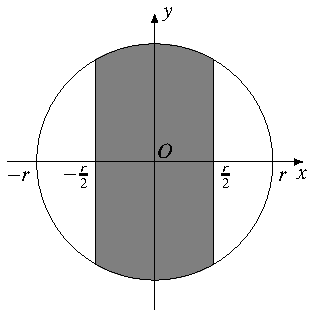
\includegraphics{fig3-1-4.pdf}
\caption{$p(x,y)$ 的非零区域与有关事件的交集部分}\label{fig:3.1.4}
\end{figure}

\textbf{四、二元正态分布}

如果二维随机变量 $(X,Y)$ 的联合密度函数 (见图~\ref{fig:3.1.5}) 为
	\begin{equation}\label{eq:3.1.8}
	\begin{aligned}
	p(x, y) &=\frac{1}{2 \pi \sigma_{1} \sigma_{2} \sqrt{1-\rho^{2}}} \exp \bigg\{-\frac{1}{2\left(1-\rho^{2}\right)}
	\bigg[\frac{\left(x-\mu_{1}\right)^{2}}{\sigma_{1}^{2}}		\\
	&-2 \rho \frac{\left(x-\mu_{1}\right)\left(y-\mu_{2}\right)}{\sigma_{1} \sigma_{2}}+\frac{\left(y-\mu_{2}\right)^{2}}{\sigma_{2}^{2}}
	\bigg] \bigg\}, \quad-\infty<x, y<+\infty \\
	\end{aligned}
	\end{equation}
则称 $(X,Y)$ 服从二元正态分布, 记为 $(X,Y)\sim N(\mu_1,\mu_2,\sigma_1^2,\sigma_2^2,\rho)$. 其中五个参数的取值范围分别是:
	\[
	 	-\infty<\mu_{1}, \mu_{2}<+\infty; \quad \sigma_{1}, \sigma_{2}>0 ; \quad-1 \leq \rho \leq 1.
	\]
	以后将指出: $\mu_1,\mu_2$ 分别是 $X$ 与 $Y$ 的均值, $\sigma_1^2,\sigma_2^2$ 分别是 $X$ 与 $Y$ 的方差, $\rho$ 是
	 $X$ 与 $Y$ 的相关系数.

	 二元正态密度函数的图形很像一顶四周无限延伸的草帽, 其中心点在 $(\mu_1,\mu_2)$ 处, 其等高线是椭圆.

	 \begin{figure}[htbp]
	 	\centering
	 	\begin{tikzpicture}[thick]
  \node (a) {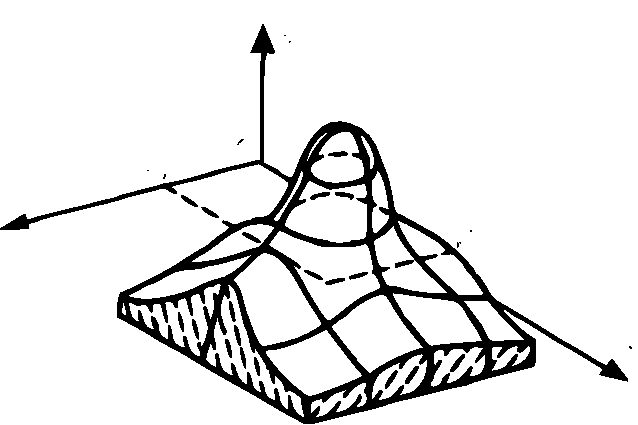
\includegraphics{fig3-1-5}};
  \fill (0,0) circle (4pt);
  \coordinate (O) at (-1.4,1.4);
  \fill[red] (-1.4,1.4) circle(2pt);
  \draw[white,line width=3pt] (O) -- ++ (-4.5,-1.05);
  \draw[white,line width=5pt] (O) -- ++ (-4.5,-1.2);
  \draw [white,line width=12pt] (O) -- ++ (0,3);
  \draw [white,line width=5pt] (O) -- ++(0.46,-0.38);
  \draw [white,line width=4pt](4.4,-2.1) -- (2.6,-1);
  \fill [white] (4.4,-2)circle(0.5cm);
  \fill [white] (2,-0.05) circle(0.1);
  \draw [-Stealth] (O) -- ++ (-4.5,-1.3) node[above]{$x$};
  \draw [-Stealth] (O)node[above left]{$O$} -- ++ (0,3) node[right]{$p(x,y)$};
  \draw (-3,1.2) node{$\mu_1$} (2.15,-0.05)node{$\mu_2$};
  \draw [-Stealth] (O) -- ++(0.5,-0.3) (2.6,-1)--(4.4,-2.2)node[above right]{$y$};
\end{tikzpicture}
	 	\caption{二元正态密度函数}\label{fig:3.1.5}
	 \end{figure}

	 \begin{example}\label{exam:3.1.7}
	 	设二维随机变量 $(X,Y)\sim N(\mu_1,\mu_2,\sigma_1^2,\sigma_2^2,\rho)$, 求 $(x,Y)$ 落在区域
	 	\[
	 	 	D=\left\{(x, y) ; \frac{\left(x-\mu_{1}\right)^{2}}{\sigma_{1}^{2}}-2 \rho \frac{\left(x-\mu_{1}\right)\left(y-\mu_{2}\right)}{\sigma_{1} \sigma_{2}}+\frac{\left(y-\mu_{2}\right)^{2}}{\sigma_{2}^{2}} \leqslant \lambda^{2}\right\}
	 	\]
	 	内的概率.
	 \end{example}
	 \begin{solution}
	 	所求的概率为
	 	\begin{equation*}
			\begin{aligned}
			p(x, y) &=\frac{1}{2 \pi \sigma_{1} \sigma_{2} \sqrt{1-\rho^{2}}} \iint_D \exp \bigg\{-\frac{1}{2\left(1-\rho^{2}\right)}
			\bigg[\frac{\left(x-\mu_{1}\right)^{2}}{\sigma_{1}^{2}}		\\
			&-2 \rho \frac{\left(x-\mu_{1}\right)\left(y-\mu_{2}\right)}{\sigma_{1} \sigma_{2}}+\frac{\left(y-\mu_{2}\right)^{2}}{\sigma_{2}^{2}}
			\bigg] \bigg\} \dd x \dd y\\
			\end{aligned}
		\end{equation*}
		作变换
		\[
		 	\begin{cases}
		 		u =\frac{x-\mu_1}{\sigma_1}-\rho \frac{y-\mu_2}{\sigma_2},\\
		 		v =\frac{y-\mu_2}{\sigma_2}\sqrt{1-\rho^2}.
		 	\end{cases}
		\]
		则可得
		\[
		 	\frac{\partial(u, v)}{\partial(x, y)}= \begin{vmatrix}{\frac{1}{\sigma_{1}}} & {0} \\
		 	{-\frac{\rho}{\sigma_{2}}} & {\frac{\sqrt{1-\rho^{2}}}{\sigma_{2}}}\end{vmatrix}=\frac{\sqrt{1-\rho^{2}}}{\sigma_{1} \sigma_{2}}, \quad|J|=\frac{\sigma_{1} \sigma_{2}}{\sqrt{1-\rho^{2}}},
		\]
		由此得
		\[
		 	p=\frac{1}{2 \pi(1-\rho^{2})} \iint_{x^{2}+v^{2} \leq \lambda^{2}} \exp \left\{-\frac{u^{2}+v^{2}}{2\left(1-\rho^{2}\right)}\right\} \dd u \dd v
		\]
		再作极坐标变换
		\[
		 	\begin{cases}
		 		u=r \sin \alpha ,\\
		 		v=r \cos \alpha	,
		 	\end{cases}
		\]
		则可得
		\[
		 	J=\frac{\partial(u, v)}{\partial(r, \alpha)}=
		 	\begin{vmatrix}
		 	{\sin \alpha} & {\cos \alpha} \\
		 	{r \cos \alpha} & {-r \sin \alpha}
		 	\end{vmatrix}=-r\left(\sin ^{2} \alpha+\cos ^{2} \alpha\right)=-r,
		\]
		最后得
		\[
		 	\begin{aligned}
		 	p &=\frac{1}{2 \pi (1-\rho^{2})} \int_{0}^{2 \pi} \dd \alpha \int_{0}^{\lambda} r \exp \left\{-\frac{r^{2}}{2\left(1-\rho^{2}\right)}\right\} \dd r \\
		 	&=\int_{0}^{\lambda} \exp \left\{-\frac{r^{2}}{2\left(1-\rho^{2}\right)}\right\}\dd \left(\frac{r^{2}}{2\left(1-\rho^{2}\right)}\right)\\
		 	&=\left.-\exp \left\{-\frac{r^{2}}{2\left(1-\rho^{2}\right)}\right\}\right|_{0} ^{\lambda}=1-\exp \left\{-\frac{\lambda^{2}}{2\left(1-\rho^{2}\right)}\right\} .
		 	\end{aligned}
		\]
	 \end{solution}

	 \begin{xiti}
	 	\item 一批产品中有一等品 50\%, 二等品 30\%, 三等品 20\%. 从中有放回地抽取 5 件, 以 $X$、$Y$ 分别表示取出的 5 件中一等品、二等品的件数,
	 	求 $(X,Y)$ 的联合分布列.
	 	\item 100 件产品中有 50 件一等品, 30 件二等品, 20 件三等品. 从中不放回地抽取 5 件, 以 $X$、$Y$ 分别表示取出的 5 件中一等品、二等品的件数,
	 	求 $(X,Y)$ 的联合分布列.
	 	\item 盘子里装有 3 只黑球、2 只红球、2 只白球, 从中任取 4 只, 以 $X$ 表示取到黑球的只数, 以 $Y$ 表示取到红球的只数,试求 $P\{X=Y\}$.
	 	\item 设随机变量 $X_i$,$i=1,2$, 的分布列如下, 且满足 $P(X_1X_2=0) =1$, 试求 $P(X_1=X_2)$.
	 	\begin{center}
	 		\begin{tabularx}{0.8\textwidth}{Z|ZZZ}
	 		$X_t$&	-1&		0&		1	\\
	 		\hline
	 		$P$	&	0.25&	0.5&	0.25	\\
	 	\end{tabularx}
	 	\end{center}
	 	\item 设随机变量 $(X,Y)$ 的联合密度函数为
	 	\[
	 	 	p(x, y)=\begin{cases}k(6-x-y),\quad & 0<x<2,2<y<4 \\
	 	 	 0,				&	\text{其他} .
	 	 	\end{cases}
	 	\]
	 	试求
	 	\begin{enumerate}[(1)]
	 		\item 常数 $k$;
	 		\item $P\{X<1,Y<3\}$;
	 		\item $P\{X<1.5\}$;
	 		\item $P\{X+Y\leq 4\}$.
	 	\end{enumerate}
	 	\item 设随机变量 $(X,Y)$ 的联合密度函数为
	 	\[
	 	 	p(x, y)=\begin{cases}
	 	 				k \ee^{-(3 x+4 y)},&	x>0,y>0 \\
	 	 	 			0,		&		\text{其他} .
	 	 	 		\end{cases}
	 	\]
	 	试求
	 	\begin{enumerate}[(1)]
	 		\item 常数 $k$;
	 		\item $(X,Y)$ 的联合分布函数 $F(X,Y)$;
	 		\item $P\{0<X\leq 1,0<Y\leq 2\}$.
	 	\end{enumerate}
	 	\item 设二维随机变量 $(X,Y)$ 的联合密度函数为
	 	\[
	 	 	p(x, y)=\begin{cases}
	 	 				4 x y,&	0<x<1,0<y<1, \\
	 	 				0,&		\text{其他} .
	 	 			\end{cases}
	 	\]
	 	试求
	 	\begin{enumerate}[(1)]
	 		\item $P(0<X<0.5,0.25<Y<1)$;
	 		\item $P(X+Y)$;
	 		\item $P(X<Y)$;
	 		\item $(X,Y)$ 的联合分布函数.
	 	\end{enumerate}
	 	\item 设二维随机变量 $(X,Y)$ 的联合密度函数为
	 	\[
	 	 	p(x,y)=\begin{cases}
	 	 		k,&		0<x^2<y<x<1;\\
	 	 		0,&		\text{其他} .
	 	 	\end{cases}
	 	\]
	 	\begin{enumerate}[(1)]
	 		\item 试求常数 $k$;
	 		\item 求 $P(X>0.5)$ 和 $P(Y<0.5)$.
	 	\end{enumerate}
	 	\item 设二维随机变量 $(X,Y)$ 的联合密度函数为
	 	\[
	 	 	p(x,y)=\begin{cases}
	 	 		6 (1-y),&	0<x<y<1;	\\
	 	 		0,&			\text{其他} .
	 	 	\end{cases}
	 	\]
	 	\begin{enumerate}[(1)]
	 		\item 求 $P(X>0.5,Y>0.5)$;
	 		\item 求 $P(X<0.5)$ 和 $P(Y<0.5)$;
	 		\item 求 $P(X+Y)<1$.
	 	\end{enumerate}
	 	\item 设随机变量 $Y$ 服从参数为 $\lambda=1$ 的指数分布, 定义随机变量 $X_k$ 如下
	 	\[
	 	 	X_k=\begin{cases}
	 	 		0,&		Y\leq k, \\
	 	 		1,&		Y>k,
	 	 	\end{cases} \quad k=1,2.
	 	\]
	 	求 $X_1$ 和 $X_2$ 的联合分布列.
	 	\item 设二维随机变量 $(X,Y)$ 的联合密度函数为
	 	\[
	 	 	p(x,y)=\begin{cases}
	 	 		x^2+\frac{xy}{3},&	0<x<1,0<y<2;\\
	 	 		0,		&			\text{其他} .
	 	 	\end{cases}
	 	\]
	 	求 $P(X+Y)\geq 1$.
	 	\item 设二维随机变量 $(X,Y)$ 的联合密度函数为
	 	\[
	 	 	p(x,y)=\begin{cases}
	 	 		\ee^{-y},	&	0<x<y;\\
	 	 		0&			\text{其他} .
	 	 	\end{cases}
	 	\]
	 	试求 $P(X,Y)\leq 1$.
	 	\item 设二维随机变量 $(X,Y)$ 的联合密度函数为
	 	\[
	 	 	p(x,y)=\begin{cases}
	 	 		1/2,&	0<x<1,0<y<2;\\
	 	 		0,&		\text{其他} .	
	 	 	\end{cases}
	 	\]
	 	求 $X$ 与 $Y$ 中至少一个小于 0.5 的概率.
	 	\item 从 (0,1) 中随机地取两个数, 求其积不小于 3/16, 且其和不大于 1 的概率.
	 \end{xiti}

	\section{边际分布与随机变量的独立性}\label{sec:3.2}
  二维联合分布函数(二维联合分布列、二维联合密度函数也一样)含有丰富的信息, 主要有以下三方面信息:
  \begin{itemize}
  	\item 每个分量的分布(每个分量的所有信息), 即边际分布.
  	\item 两个分量之间的关联程度, 即协方差和相关系数.
  	\item 给定一个分量时, 另一个分量的分布, 即条件分布.
  \end{itemize}
  我们的目的时将这些信息从联合分布中挖掘出来, 本节先讨论边际分布.

  \subsection{边际分布函数}\label{ssec:3.2.1}
  如果在二维随机变量 $(X,Y)$ 的联合分布函数 $F(X,Y)$ 中令 $y\to+\infty$ , 由于 $|Y<+\infty|$ 为必然事件, 故可得
  \begin{equation*}
  \lim_{y\to+\infty}F(x,y)=P(X\leqslant x,Y<+\infty)=P(X\leqslant x),
  \end{equation*}
  这是一个分布函数, 被称为 $X$ 的\textbf{边际分布}, 记为
  \begin{equation}
  F_{X}(x)=F(x,+\infty).\label{eq:3.2.1}
  \end{equation}
  类似地, 在 $F(x,y)$ 中令 $x\to+\infty$ , 可得 $Y$ 的\textbf{边际分布}
  \begin{equation}
  F_{Y}(y)=F(+\infty,y).\label{eq:3.2.2}
  \end{equation}
  在三维随机变量 $(X,Y,Z)$ 的联合分布函数 $F(x,y,z)$ 中, 用类似的方法可得到更多的边际分布函数:
  \begin{align*}
  &F_{X}(x) = F(x,+\infty,+\infty);\\
  &F_{Y}(y) = F(+\infty,y,+\infty);\\
  &F_{Z}(z) = F(+\infty,+\infty,z);\\
  &F_{X,Y}(x,y) = F(x,y,+\infty);\\
  &F_{X,Z}(x,z) = F(x,+\infty,z);\\
  &F_{Y,Z}(y,z) = F(+\infty,y,z).
  \end{align*}
  在更高维的场合, 也可类似地从联合分布函数获得其低维的边际分布函数.
  \begin{example}\label{exam:3.2.1}
  	设二维随机变量 $(X,Y)$ 的联合分布函数为
  	\begin{equation*}
  	F(x,y)=
  	\begin{cases}
  	1-\ee^{-x}-\ee^{-y}+\ee^{-x-y-\lambda xy}, & x>0,y>0;\\
  	0, & \text{其他}.
  	\end{cases}
  	\end{equation*}
  	这个分布被称为二维指数分布, 其中参数 $\lambda>0$.
  	
  	由此联合分布函数 $F(x,y)$ , 容易获得 $X$ 与 $Y$ 的边际分布函数为
  	\begin{align*}
  	F_{X}(x) &= F(x,+\infty)=
  	\begin{cases}
  	1-\ee^{-x}, & x>0;\\
  	0, & x\leqslant0.
  	\end{cases}\\
  	F_{Y}(y) &= F(+\infty,y)=
  	\begin{cases}
  	1-\ee^{-y}, & y>0;\\
  	0, & y\leqslant0.
  	\end{cases}
  	\end{align*}
  	它们都是一维指数分布, 且与参数 $\lambda>0$ 无关. 不同的 $\lambda>0$ 对应不同的二维指数分布, 但它们的两个边际分布不变. 这说明: 二维联合分布不仅含有每个分量的概率分布, 而且还含有两个变量 $X$ 与 $Y$ 间关系的信息, 这正是人们要研究多维随机变量的原因.
  \end{example}

  \subsection{边际分布列}\label{ssec:3.2.2}
  在二维离散随机变量 $(X,Y)$ 的联合分布列 $\left\{P(X=x_i,Y=y_i)\right\}$ 中, 对 $j$ 求和所得的分布列
  \begin{equation}
  \sum_{j=1}^{+\infty}P(X=x_i,Y=y_j)=P(X=x_i), i=1,2,\ldots\label{eq:3.2.3}
  \end{equation}
  被称为 $X$ 的边际分布列. 类似地, 对 $i$ 求和所得的分布列
  \begin{equation}
  \sum_{i=1}^{+\infty}P(X=x_i,Y=y_j)=P(Y=y_j), j=1,2,\ldots\label{eq:3.2.4}
  \end{equation}
  被称为 $Y$ 的边际分布列.
  \begin{example}\label{exam:3.2.2}
  	设二维随机变量 $(X,Y)$ 有如下的联合分布列
  	\begin{equation*}
  	\begin{tabularx}{0.8\textwidth}{ZZZZ}
  	\toprule
  	 & \multicolumn{3}{c}{$Y$}\\
  	\cmidrule{2-4}
  	$X$ & 1 & 2 & 3\\
  	\midrule
  	0 & 0.09 & 0.21 & 0.24\\
  	1 & 0.07 & 0.12 & 0.27\\
  	\bottomrule
  	\end{tabularx}
  	\end{equation*}
  	求 $X$ 与 $Y$ 的边际分布列.
  	\end{example}

  \begin{solution}
  	在上述联合分布列中, 对每一行求和得 $0.54$ 与 $0.46$ , 并把它们写在对应行得右侧, 这就是 $X$ 的边际分布列. 再对每一列求和, 得 $0.16,0.33$ 和 $0.51$ , 并把它们写在对应列的下侧, 这就是 $Y$ 得边际分布列.
  	\begin{equation*}
  	\begin{tabularx}{0.8\textwidth}{ZZZZZ}
  	\toprule
  	 & \multicolumn{3}{c}{$Y$} & \\
  	 \cmidrule{2-4}
  	$X$ & 1 & 2 & 3 & $P(X=i)$ \\
  	\midrule
  	0 & 0.09 & 0.21 & 0.24 & 0.54 \\
  	1 & 0.07 & 0.12 & 0.27 & 0.46 \\
  	\midrule
  	$P(Y=j)$ & 0.16 & 0.33 & 0.51 &1\\
  	\bottomrule
  	\end{tabularx}
  	\end{equation*}
  \end{solution}

  \subsection{边际密度函数}\label{ssec:3.2.3}
  如果二维连续随机变量 $(X,Y)$ 的联合密度函数为 $p(x,y)$ , 因为
  \begin{align*}
  F_{X}(x) &= F(x,+\infty)=\int_{-\infty}^{x}\left( \int_{-\infty}^{+\infty}p(u,v)\,\dd v \right)\,\dd u=\int_{-\infty}^{x}p_{X}(u)\,\dd u,\\
  F_{Y}(y) &= F(+\infty,y)=\int_{-\infty}^{y}\left( \int_{-\infty}^{+\infty}p(u,v)\,\dd u \right)\,\dd v=\int_{-\infty}^{y}p_{Y}(v)\,\dd v,
  \end{align*}
  其中 $p_{X}(x)$ 和 $p_{Y}(y)$ 分别为
  \begin{align}
  p_{X}(x) &= \int_{-\infty}^{+\infty}p(x,y)\,\dd y.\label{eq:3.2.5}\\
  p_{Y}(y) &= \int_{-\infty}^{+\infty}p(x,y)\,\dd x.\label{eq:3.2.6}
  \end{align}
  它们恰好处于密度函数位置, 故称上式给出的 $p_{X}(x)$ 为 $X$ 的边际密度函数, $p_{Y}(y)$ 为 $Y$ 的边际密度函数.

  由联合密度函数求边际密度函数时, 要注意积分区域的确定.
  \begin{example}\label{exam:3.2.3}
  	设二维随机变量 $(X,Y)$ 的联合密度函数为
  	\begin{equation*}
  	p(x,y)=
  	\begin{cases}
  	1, & 0<x<1,|y|<x;\\
  	0, & \text{其他}.
  	\end{cases}
  	\end{equation*}
  	试求:(1)边际密度函数 $p_{X}(x)$ 和 $p_{Y}(y)$;(2) $P(X<1/2)$ 及 $P(Y>1/2)$ .
  \end{example}
  \begin{solution}
  	首先识别 $p(x,y)$ 的非零区域, 它如图~\ref{fig:3.2.1} 所示.
  	\begin{figure}[htbp]
  		\centering
  		\begin{tikzpicture}[scale=1.5,>=Stealth]
  		  \draw[->] (-1,0) -- (0,0)
            node[below left] {$O$} -- (1,0)
            node[below right]{1} -- (1.5,0)node[below] {$x$};
          \draw [->] (0,-1.5) -- (0,-1) node[left] {$-1$}
          -- (0,1) node[left] {1} -- (0,1.5) node[right] {$y$};
          \filldraw [pattern=vertical lines,thick] (0,0) -- (1,-1) -- (1,1) -- cycle;
          \draw [densely dashed] (1,1) -- (0,1) (1,-1) -- (0,-1);
  		\end{tikzpicture}
  		\caption{$p(x,y)$ 的非零区域}\label{fig:3.2.1}
  	\end{figure}
  	\begin{itemize}
  		\item[(1)]求 $p_X(x)$: 当 $x\leqslant0$ 或 $x\geqslant1$ 时, 有 $p_X(x)=0$. 而当 $0<x<1$ 时, 有
  		\begin{equation*}
  		p_X(x)=\int_{-\infty}^{+\infty}p(x,y)\,\dd y=\int_{-x}^{x}\,\dd y=2x.
  		\end{equation*}
  		所以 $X$ 的边际密度函数为(见图~\ref{fig:3.2.2}~)
  		\begin{equation*}
  		p_X(x)=
  		\begin{cases}
  		2x, & 0<x<1;\\
  		0, & \text{其他}.
  		\end{cases}
  		\end{equation*}
  		\begin{figure}[h]
  			\centering
  			\begin{tikzpicture}[>=Stealth,scale=1.2]
              \draw [->] (-0.8,0) -- (0,0) node[below left] {$O$} -- (1,0) node[below] {1} -- (2.5,0)node[below] {$x$};
              \draw [->] (0,-0.3) -- (0,2) node[left]{2}
               -- (0,2.5) node[right]{$p_X(x)$};
              \draw (0,1) node[left]{1} -- (0.05,1);
              \draw [thick] (0,0) -- (1,2);
              \draw[densely dashed] (1,0) -- (1,2) -- (0,2);
  			\end{tikzpicture}
  			\caption{$X$ 的边际密度函数}\label{fig:3.2.2}
  		\end{figure}
  		再求 $p_Y(y):$ 当 $y\leqslant-1$ 或 $y\geqslant1$ 时, 有 $p_Y(y)=0$. 而当 $-1<y<0$ 时, 有
  		\begin{equation*}
  		p_Y(y)=\int_{-\infty}^{+\infty}p(x,y)\,\dd x=\int_{-y}^{1}\,\dd x=1+y,
  		\end{equation*}
  		当 $0<y<1$ 时, 有
  		\begin{equation*}
  		p_Y(y)=\int_{-\infty}^{+\infty}p(x,y)\,\dd x=\int_{y}^{1}\,\dd x=1-y.
  		\end{equation*}
  		所以 $Y$ 的边际密度函数为(见图~\ref{fig:3.2.3}~)
  		\begin{equation*}
  		p_{Y}(y)=
  		\begin{cases}
  		1+y, & -1<y<0,\\
  		1-y, & 0<y<1,\\
  		0, & \text{其他}.
  		\end{cases}
  		\end{equation*}
  		\begin{figure}[h]
  			\centering
  			\begin{tikzpicture}[scale=2,>=Stealth]
  			  \draw [->] (-1.5,0) -- (-1,0)
                node[below] {$-1$} -- (0,0) node[below left] {$O$} -- (1,0)node[below] {1} -- (1.5,0)node[below] {$y$};
                \draw [->] (0,-0.5) -- (0,0.5) node[above right] {0.5} -- (0,1) node[right] {$p_Y(y)$};
                \draw (-1,0) -- (0,0.5) -- (1,0);
  			\end{tikzpicture}
  			\caption{ $Y$ 的边际密度函数}\label{fig:3.2.3}
  		\end{figure}
  		\item[(2)] 要求的概率分别为
  		\begin{align*}
  		P(X<1/2) &= \int_{-\infty}^{1/2}p_{X}(x)\,\dd x=\int_{0}^{1/2}2x\,\dd x=\frac{1}{4}.\\
  		P(Y>1/2) &= \int_{1/2}^{+\infty}p_{Y}(y)\,\dd y=\int_{1/2}^{1}(1-y)\,\dd y=\frac{1}{8}.
  		\end{align*}
  	\end{itemize}
  \end{solution}

  \begin{example}\label{exam:3.2.4}
  	\textbf{多项分布的边际分布仍为多项分布}
  \end{example}
  \begin{solution}
  	下面只证三项分布的边际分布为二项分布. 设 $(X,Y)$ 服从三项分布 $M(n,p_1,p_2,p_3),$  其联合分布列为
  	\begin{equation*}
  	P(X=i,Y=j)=\frac{n!}{i!j!(n-i-j)!}p_1^ip_2^j(1-p_1-p_2)^{n-i-j}, i,j=1,2,\ldots,n,i+j\leqslant n.
  	\end{equation*}
  	对上式分别乘以和除以 $(1-p_1)^{n-i}/(n-i)!$ , 再对 $j$ 从 $0$ 到 $n-1$ 求和, 并记 $p_2'=p_2/(1-p_1)$, 则可得
  	\begin{align*}
  	&\sum_{j=0}^{n-i}P(X=i,Y=j) = \frac{n!}{i!(n-i)!}p_1^i(1-p_1)^{n-i}.\\
  	&\sum_{j=0}^{n-i} \Binom{n-i}{j} \left(\frac{p_2}{1-p_1}\right)^{j}\left(1-\frac{p_2}{1-p_1}\right)^{n-i-j} \\
  	&= \frac{n!}{i!(n-i)!}p_1^i(1-p_1)^{n-i}\left[p_2'+(1-p_2')\right]^{n-i}\\
  	&= \frac{n!}{i!(n-i)!}p_1^i(1-p_1)^{n-i}.
  	\end{align*}
  	所以 $X\sim b(n,p_1)$ . 同理可证 $Y\sim b(n,p_2)$.
  	
  	用类似的方法可以证明: 若 $(X_,,X_2,\ldots,X_r)\sim M(n,p_1,p_2,\ldots,p_r)$, 则 $X_i\sim b(n,p_i), i=1,2,\ldots,r$.
  \end{solution}

  \begin{example}\label{exam:3.2.5}
  	\textbf{二维正态分布的边际分布为一维正态分布}
  \end{example}
  \begin{solution}
  	设 $(X,Y)\sim N(\mu_1,\mu_2,\sigma_1^2,\sigma_2^2,\rho)$ . 先把 ~\eqref{eq:3.1.8}~式二维正态密度函数 $p(x,y)$ 的指数部分
  	\begin{equation*}
  	-\frac{1}{2(1-\rho^2)}\left[\frac{(x-\mu_1)^2}{\sigma_1^2}-2\rho\frac{(x-\mu_1)(y-\mu_2)}{\sigma_1\sigma_2}+\frac{(y-\mu_2)^2}{\sigma_2^2}\right]
  	\end{equation*}
  	改写成
  	\begin{equation*}
  	-\frac{1}{2}\left[\rho\frac{x-\mu_1}{\sigma_1\sqrt{1-\rho^2}}-\frac{y-\mu_2}{\sigma_2\sqrt{1-\rho^2}}\right]^2-\frac{(x-\mu_1)^2}{2\sigma_1^2}.
  	\end{equation*}
  	再对积分
  	\begin{equation*}
  	\int_{-\infty}^{+\infty}\exp\left\{-\frac{1}{2}\left[\rho\frac{x-\mu_1}{\sigma_1\sqrt{1-\rho^2}}-\frac{y-\mu_2}{\sigma_2\sqrt{1-\rho^2}}\right]^2\right\}\,\dd y
  	\end{equation*}
  	作变换(注意把 $x$ 看作常量)
  	\begin{equation*}
  	t=\rho\frac{x-\mu_1}{\sigma_1\sqrt{1-\rho^2}}-\frac{y-\mu_2}{\sigma_2\sqrt{1-\rho^2}},
  	\end{equation*}
  	则
  	\begin{align*}
  	p_{X}(x) &= \int_{-\infty}^{+\infty}p(x,y)\,\dd y\\
  	&=\frac{1}{2\uppi\sigma_1\sigma_2\sqrt{1-\rho^2}}\exp\left\{-\frac{(x-\mu_1)^2}{2\sigma_1^2}\right\}\sigma_2\sqrt{1-\rho^2}\int_{-\infty}^{+\infty}\exp\left\{-\frac{t^2}{2}\right\}\,\dd t.
  	\end{align*}
  	注意到上式中的积分恰好等于 $\sqrt{2\uppi}$ , 所以有
  	\begin{equation*}
  	p_{X}(x)=\frac{1}{\sqrt{2\uppi}\sigma_1}\exp\left\{-\frac{(x-\mu_1)^2}{2\sigma_1^2}\right\}.
  	\end{equation*}
  	这正是一维正态分布 $N(\mu_1,\sigma_1^2)$ 的密度函数, 即 $X\sim N(\mu_1,\sigma_1^2)$ . 同理可证 $Y\sim N(\mu_2,\sigma_2^2)$ . 由此可见
  	\begin{itemize}
  		\item 二维正态分布的边际分布中不含参数 $\rho$ .
  		\item 这说明二维正态分布 $N(\mu_1,\mu_2,\sigma_1^2,\sigma_2^2,0.1)$ 与 $N(\mu_1,\mu_2,\sigma_1^2,\sigma_2^2,0.2)$ 的边际分布是相同的.
  		\item 具有相同边际分布的多维联合分布可以是不同的.
  	\end{itemize}
  \end{solution}

   \subsection{随机变量间的独立性}\label{ssec:3.2.4}
   在多维随机变量中, 各分量的取值有时会相互影响, 但有时毫无影响. 譬如一个人的身高 $X$ 和体重 $Y$ 就会相互影响, 但与收入 $Z$ 一般无影响. 当两个随机变量取值的规律互不影响时, 就称它们是相互独立的.
   \begin{definition}{}{3.2.1}
   	设 $n$ 维随机变量 $(X_1,X_2,\ldots,X_n)$ 的联合分布函数为 $F(x_1,x_2,\ldots,x_n)$ , $F_i(x_i)$ 为 $X_i$ 的边际分布函数. 如果对任意 $n$ 个实数 $x_1,x_2,\ldots,x_n$ , 有
   	\begin{equation}\label{eq:3.2.7}
   		F(x_1,x_2,\ldots,x_n)=\prod_{i=1}^{n}F_i(x_i),
   	\end{equation}
   	则称 $X_1,X_2,\ldots,X_n$ \textbf{相互独立}.
   \end{definition}
   在离散随机变量场合, 如果对其任意 $n$ 个取值 $x_1,x_2,\ldots,x_n$ , 有
   \begin{equation}\label{eq:3.2.8}
   	P(X_1=x_1,X_2=x_2,\ldots,X_n=x_n)=\prod_{i=1}^{n}P(X_i=x_i),
   \end{equation}
   则称 $X_1,X_2,\ldots,X_n$ 相互独立.

   在连续随机变量场合, 如果对任意 $n$ 个实数 $x_1,x_2,\ldots,x_n$ , 有
   \begin{equation}\label{eq:3.2.9}
   	p(x_1,x_2,\ldots,x_n)=\prod_{i=1}^{n}p_i(x_i),
   \end{equation}
   则称 $X_1,X_2,\ldots,X_n$ 相互独立.

   \begin{example}
   	设 $(X,Y)$ 是二维离散随机变量, $X$ 和 $Y$ 的边际分布列分别如下所示:
   	\begin{table}[h]
   		\centering
   		\begin{tabularx}{0.4\textwidth}{Z|ZZZ}
   			\hline
   			$X$ & $-1$ & $0$ & $1$\\
   			\hline
   			$P$ & $1/4$ & $1/2$ & $1/4$\\
   			\hline
   		\end{tabularx}
   	    \qquad
   	    \begin{tabularx}{0.4\textwidth}{Z|ZZ}
   	    	\hline
   	    	$Y$ & $0$ & $1$\\
   	    	\hline
   	    	$P$ & $1/2$ & $1/2$\\
   	    	\hline
   	    \end{tabularx}
   	\end{table}
   如果 $P\left\{XY=0\right\}=1$, 试求

   (1) $(X,Y)$ 的联合分布列;

   (2) $X$ 与 $Y$ 是否独立?

   \end{example}
   \begin{solution}
   	\begin{itemize}
   		\item[(1)] 记 $(X,Y)$ 得联合分布列如下, 其中 $p_{ij}=P(X=i,Y=j)$ , 在联合分布列的右侧是 $X$ 的边际分布列, 下侧是 $Y$ 的边际分布列.
   		\begin{center}
   			\begin{tabularx}{0.8\textwidth}{XXXX}
   				\toprule
   				 & \multicolumn{2}{c}{$Y$} & \\
   				\cmidrule{2-3}
   				$X$ & $0$ & $1$ & $P(X=i)$\\
   				\midrule
   				$-1$ & $p_{11}$ & $p_{12}$ & $1/4$\\
   				$0$ & $p_{21}$ & $p_{22}$ & $1/2$\\
   				$1$ & $p_{31}$ & $p_{32}$ & $1/4$\\
   				\midrule
   				$P(Y=j)$ & $1/2$ & $1/2$ & $1$\\
   				\bottomrule
   			\end{tabularx}
   		\end{center}
   		由 $P(XY=0)=1$ , 知 $P(XY\ne0)=0$ , 即
   		\begin{equation*}
   		p_{12}=P(X=-1,Y=1)=0,\quad p_{32}=P(X=1,Y=1)=0.
   		\end{equation*}
   		其余四个概率可由下面等式分别确定.
   		\begin{center}
   			\begin{tabular}{l}
   				从表中第一行看, 由 $p_{11}+p_{12}=1/4$ , 得 $p_{11}=1/4$ .\\
   				从表中第三行看, 由 $p_{31}+p_{32}=1/4$ , 得 $p_{31}=1/4$ .\\
   				从表中第一列看, 由 $p_{11}+p_{21}+p_{31}=1/2=1/4+p_{21}+1/4$ , 得 $p_{21}=0$ .\\
   				从表中第二列看, 由 $p_{12}+p_{22}+p_{32}=1/2=0+p_{22}+0$ , 得 $p_{22}=1/2$ .
   			\end{tabular}
   		\end{center}
   		
   		于是得 $(X,Y)$ 的联合分布列如下:
   		\begin{center}
   			\begin{tabularx}{0.8\textwidth}{YYYY}
   				\toprule
   				 & \multicolumn{2}{c}{$Y$} & \\
   				\cmidrule{2-3}
   				X & 0 & 1 & p_{i\cdot}\\
   				\midrule
   				-1 & 1/4 & 0 & 1/4\\
   				0 & 0 & 1/2 & 1/2\\
   				1 & 1/4 & 0 & 1/4\\
   				\midrule
   				p_{\cdot j} & 1/2 & 1/2 & 1\\
   				\bottomrule
   			\end{tabularx}
   		\end{center}
   		\item[(2)] 因为 $P(X=0,Y=0)=p_{21}=0$ , 而 $P(X=0)P(Y=0)=1/4$ , 所以 $X$ 与 $Y$ 不独立.
   	\end{itemize}
   \end{solution}

   \begin{example}\label{exam:3.2.7}
   	若 $(X,Y)$ 的联合密度函数为
   	\begin{equation*}
   		p(x,y)=
   		\begin{cases}
   		8xy, & 0\leqslant x\leqslant y\leqslant1;\\
   		0, & \text{其他}.
   		\end{cases}
   	\end{equation*}
   	问 $X$ 与 $Y$ 是否相互独立?
   \end{example}
   \begin{solution}
   	为判断 $X$ 与 $Y$ 是否独立, 只需看边际密度函数的乘积是否等于联合密度函数. 为此先求边际密度函数.
   	当 $x<0$ 或 $x>1$ 时, $p_{X}(x)=0$ . 而当 $0\leqslant x\leqslant1$ 时, 有
   	\begin{equation*}
   		p_{X}(x)=\int_{x}^{1}8xy\,\dd y=8x\left(\frac{1}{2}-\frac{x^2}{2}\right)=4x\left(1-x^2\right).
   	\end{equation*}
   	因此
   	\begin{equation*}
   		p_{X}(x)=
   		\begin{cases}
   		4x\left(1-x^2\right), & 0\leqslant x\leqslant1,\\
   		0, & \text{其他}.
   		\end{cases}
   	\end{equation*}
   	同样, 当 $y<0$ 或 $y>1$ 时, $p_{Y}(y)=0$ . 而当 $0\leqslant y\leqslant 1$ 时, 有
   	\begin{equation*}
   		p_{Y}(y)=\int_{0}^{x}8xy\,\dd x=4y^3.
   	\end{equation*}
   	因此
   	\begin{equation*}
   		p_{Y}(y)=
   		\begin{cases}
   		4y^3, & 0\leqslant y\leqslant1;\\
   		0, & \text{其他}.
   		\end{cases}
   	\end{equation*}
   	由此得 $p(x,y)\ne p_{X}(x)p_{Y}(y)$ , 所以 $X$ 与 $Y$ 不独立.
   \end{solution}

   \begin{example}\label{exam:3.2.8}
   	从 $(0,1)$ 中任取两个数, 求下列事件的概率.
   	
   	(1)两数之和小于 $1.2$ ;
   	
   	(2)两数之积小于 $1/4$ .
   \end{example}
   \begin{solution}
   	分别记这两个数为 $X$ 和 $Y$ , 则 $X$ 和 $Y$ 独立, 且都服从 $(0,1)$ 上的均匀分布, $(X,Y)$ 的联合密度函数为
   	\begin{equation*}
   		p(x,y)=p_{X}(x)p_{Y}(y)=
   		\begin{cases}
   		1, & 0<x<1,0<y<1;\\
   		0, & \text{其他}.
   		\end{cases}
   	\end{equation*}
   	\begin{itemize}
   		\item[(1)] 从图~\ref{fig:3.2.4a}可知
   		\begin{align*}
   			P(X+Y<1.2)=\int_{0}^{0.2}\int_{0}^{1}\,\dd y\dd x+\int_{0.2}^{1}\int_{0}^{1.2-x}\,\dd y\dd x\\
   			=0.2+\int_{0.2}^{1}(1.2-x)\,\dd x=0.2+0.48=0.68.
   		\end{align*}
   		\begin{figure}[h]
   			\centering
   			\subfloat[$\{x+y<1.2,0<x,y<1\}$]{\label{fig:3.2.4a}
   			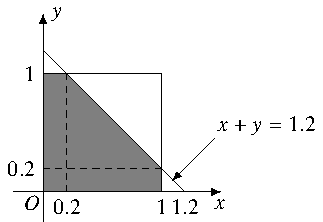
\includegraphics{fig3-2-4a.pdf}}
   			\qquad
   			\subfloat[$\{xy<1/4,0<x,y<1\}$]{\label{fig:3.2.4b}
   			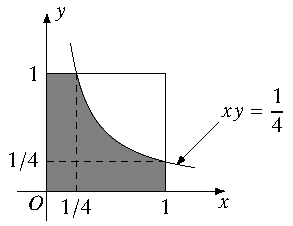
\includegraphics{fig3-2-4b.pdf}
   			}
   			\caption{ $p(x,y)$ 的非零区域与有关事件的交集部分}\label{fig:3.2.4}
   		\end{figure}
   	\item[(2)] 从图~\ref{fig:3.2.4b}可知
   	\begin{align*}
   		P(XY<1/4)=\int_{0}^{1/4}\int_{0}^{1}\,\dd y\dd x+\int_{1/4}^{1}\int_{0}^{1/(4x)}\,\dd y\dd x\\
   		=\frac{1}{4}+\int_{1/4}^{1}\frac{1}{4x}\,\dd x=\frac{1}{4}+\frac{1}{4}\ln4=0.5966.
   	\end{align*}
   	\end{itemize}
   \end{solution}

   \begin{xiti}
   		\item 设二维离散随机变量 $(X,Y)$ 的可能值为
   		\begin{equation*}
   			(0,0), (-1,1), (-1,2), (1,0).
   		\end{equation*}
   		且取这些值的概率依次为 $1/6,1/3,1/12,5/12$ , 试求 $X$ 与 $Y$ 各自的边际分布列.
   		\item 设二维随机变量 $(X,Y)$ 的联合分布函数为
   		\begin{equation*}
   			F(x,y)=\begin{cases}
   			1-\ee^{-\lambda_{1}x}-\ee^{-\lambda_{2}y}+\ee^{-\lambda_{1}x-\lambda_{2}y-\lambda_{12}\max\{x,y\}}, & x>0,y>0;\\
   			0, & \text{其他}.
   			\end{cases}
   		\end{equation*}
   		试求 $X$ 和 $Y$ 各自的边际分布函数.
   		\item 试求以下二维均匀分布的边际分布:
   		\begin{equation*}
   			p(x,y)=\begin{cases}
   			\frac{1}{\uppi}, & x^2+y^2\leqslant1;\\
   			0, & \text{其他}.
   			\end{cases}
   		\end{equation*}
   		\item 设平面区域 $D$ 由曲线 $y=1/x$ 及直线 $y=0,x=1,x=\ee^2$ 所围成, 二维随机变量 $(X,Y)$ 在区域 $D$ 上服从均匀分布, 试求 $X$ 的边际密度函数.
   		\item 求以下给出的 $(X,Y)$ 的联合密度函数的边际密度函数 $p_{X}(x)$ 和 $p_{Y}(y)$.
   		\begin{align*}
   			p_{1}(x,y) &= \begin{cases}
   			\ee^{-y}, & 0<x<y;\\
   			0, & \text{其他}.
   			\end{cases}\\
   			p_{2}(x,y) &= \begin{cases}
   			\frac{5}{4}(x^2+y), & 0<y<1-x^2;\\
   			0, & \text{其他}.
   			\end{cases}
   		\end{align*}
   		\item 设二维随机变量 $(X,Y)$ 的联合密度函数为
   		\begin{equation*}
   			p(x,y)=\begin{cases}
   			6, & 0<x^2<y<x<1;\\
   			0, & \text{其他}.
   			\end{cases}
   		\end{equation*}
   		试求边际密度函数 $p_{X}(x)$ 和 $p_{Y}(y)$ .
   		\item 试验证: 以下给出的两个不同的联合密度函数, 它们有相同的边际密度函数.
   		\begin{align*}
   			p(x,y) &= \begin{cases}
   			x+y, & 0\leqslant x\leqslant1,0\leqslant y\leqslant1;\\
   			0, & \text{其他}.
   			\end{cases}\\
   			g(x,y) &= \begin{cases}
   			(0.5+x)(0.5+y), & 0\leqslant x\leqslant1,0\leqslant y\leqslant1;\\
   			0, & \text{其他}.
   			\end{cases}
   		\end{align*}
   		\item 设随机变量 $X$ 和 $Y$ 独立同分布, 且
   		\begin{equation*}
   			P(X=-1)=P(Y=-1)=P(X=1)=P(Y=1)=\frac{1}{2}
   		\end{equation*}
   		试求 $P\{X=Y\}$ .
   		\item 甲、乙两人独立地各进行两次射击, 假设甲的命中率为 $0.2$ , 乙的命中率为 $0.5$ , 以 $X$ 和 $Y$ 分别表示甲和乙的命中次数, 试求 $P(X\leqslant Y)$ .
   		\item 设随机变量 $X$ 和 $Y$ 相互独立, 其联合分布列为
   		\begin{center}
   			\begin{tabularx}{0.8\textwidth}{ZZZZ}
   				\hline
   				 & \multicolumn{3}{c}{ $Y$ }\\
   				\cline{2-4}
   				$X$ & $y_1$ & $y_2$ & $y_3$\\
   				\hline
   				$x_1$ & $a$ & $1/9$ & $c$\\
   				\hline
   				$x_2$ & $1/9$ & $b$ & $1/3$\\
   				\hline
   			\end{tabularx}
   		\end{center}
   	
   	    试求联合分布列中的 $a,b,c$ .
   		\item 设 $k_1,k_2$ 分别是掷一枚骰子两次先后出现的点数. 试求方程 $x^2+k_1x+k_2=0$ 有实根的概率 $p$ 和有重根的概率 $q$.
   		\item 设 $X$ 与 $Y$ 是两个相互独立的随机变量, $X\sim U(0,1)$ , $Y\sim Exp(1)$ . 试求
   		\begin{itemize}
   			\item[(1)] $X$ 与 $Y$ 的联合密度函数;
   			\item[(2)] $P(Y\leqslant X)$ ;
   			\item[(3)] $P(X+Y\leqslant1)$ .
   		\end{itemize}
   	    \item 设随机变量 $(X,Y)$ 的联合密度函数为
   	    \begin{equation*}
   	    	p(x,y)=\begin{cases}
   	    	3x, & 0<x<1,0<y<x;\\
   	    	0, & \text{其他}.
   	    	\end{cases}
   	    \end{equation*}
   	    试求
   	    \begin{itemize}
   	    	\item[(1)] 边际密度函数 $p_{X}(x)$ 和 $p_{Y}(y)$ ;
   	    	\item[(2)] $X$ 与 $Y$ 是否独立?
   	    \end{itemize}
       \item 设随机变量 $(X,Y)$ 的联合密度函数为
       \begin{equation*}
       	p(x,y)=\begin{cases}
       	1, & |x|<y,0<y<1;\\
       	0, & \text{其他}.
       	\end{cases}
       \end{equation*}
       试求
       \begin{itemize}
       	\item[(1)] 边际密度函数 $p_{X}(x)$ 和 $p_{Y}(y)$ ;
       	\item[(2)] $X$ 与 $Y$ 是否独立?
       \end{itemize}
       \item 在长为 $a$ 的线段的中点的两边随机地各选取一点, 求两点间的距离小于 $a/3$ 的概率.
       \item 设二维随机变量 $(X,Y)$ 的联合密度函数为 $p(x,y)$ . 证明: $X$ 与 $Y$ 相互独立的充要条件是 $p(x,y)$ 可分离变量, 即 $p(x,y)=h(x)g(y)$ . 又问 $h(x),g(y)$ 与边际密度函数有什么关系?
   \end{xiti}
      \section{多维随机变量函数的分布}\label{sec:3.3}
   设 $(X_1,X_2,\ldots,X_n)$ 为 $n$ 维随机变量, 则 $Y=g(X_1,X_2,\ldots,X_n)$ 是 $(X_1,X_2,\ldots,X_n)$ 的函数, $Y$ 是一维随机变量. 现在的问题是如何由 $(X_1,X_2,\ldots,X_n)$ 的分布, 求出 $Y$ 的分布. 这是一类技巧性很强的工作, 不仅对离散场合和连续场合有不同的方法, 而且对不同形式的函数 $g(X_1,X_2,\ldots,X_n)$ 要采用不同的方法, 甚至有些方法只对特殊形式的 $g(\cdot)$ 适用. 下面将以例子形式讲述这些方法.
   \subsection{多维离散随机变量函数的分布}\label{ssec:3.3.1}
   设 $(X_1,X_2,\ldots,X_n)$ 为 $n$ 维离散随机变量, 则某一函数 $Y=g(X_1,X_2,\ldots,X_n)$ 是一维离散随机变量. 当 $(X_1,X_2,\ldots,X_n)$ 所有可能取值较少时, 可将 $Y$ 的取值一一列出, 然后再合并整理就可得出结果, 见下例.
   \begin{example}\label{exam:3.3.1}
   	设 $(X,Y)$ 的联合分布列如下所示:
   	\begin{center}
   		\begin{tabularx}{0.8\textwidth}{ZZZZ}
   			\hline
   			& \multicolumn{3}{c}{$Y$} \\
   			\cline{2-4}
   			$X$ & $-1$ & $1$ & $2$\\
   			\hline
   			$-1$ & $5/20$ & $2/20$ & $6/20$\\
   			$2$ & $3/20$ & $3/20$ & $1/20$\\
   			\hline
   		\end{tabularx}
   	\end{center}
   	试求:
   	\begin{itemize}
   		\item[(1)] $Z_1=X+Y$ 的分布列;
   		\item[(2)] $Z_2=X-Y$ 的分布列;
   		\item[(3)] $Z_3=\max\{X,Y\}$ 的分布列.
   	\end{itemize}
   	\begin{solution}
   		将 $(X,Y)$ 及各个函数的取值对应列于同一表中:
   		\begin{center}
   			\begin{tabular}{c|cccccc}
   				\hline
   				$P$ & $5/20$ & $2/20$ & $6/20$ & $3/20$ & $3/20$ & $1/20$\\
   				\hline
   				$(X,Y)$ & $(-1,-1)$ & $(-1,1)$ & $(-1,2)$ & $(2,-1)$ & $(2,1)$ & $(2,2)$\\
   				\hline
   				$Z_1=X+Y$ & $-2$ & $0$ & $1$ & $1$ & $3$ & $4$\\
   				\hline
   				$Z_2=X-Y$ & $0$ & $-2$ & $-3$ & $3$ & $1$ & $0$\\
   				\hline
   				$Z_3=\max\{X,Y\}$ & $-1$ & $1$ & $2$ & $2$ & $2$ & $2$\\
   				\hline
   			\end{tabular}
   		\end{center}
   		
   		然后经过合并整理就可得最后结果:
   		\begin{center}
   			\begin{tabular}{c|ccccc}
   				\hline
   				$Z_1=X+Y$ & $-2$ & $0$ & $1$ & $3$ & $4$\\
   				\hline
   				$P$ & $5/20$ & $2/20$ & $9/20$ & $3/20$ & $1/20$\\
   				\hline
   			\end{tabular}
   		\end{center}
   	    \begin{center}
   	    	\begin{tabular}{c|ccccc}
   	    		\hline
   	    		$Z_2=X-Y$ & $-3$ & $-2$ & $0$ & $1$ & $3$\\
   	    		\hline
   	    		$P$ & $6/20$ & $2/20$ & $6/20$ & $3/20$ & $3/20$\\
   	    		\hline
   	    	\end{tabular}
   	    \end{center}
       \begin{center}
       	\begin{tabular}{c|ccc}
       		\hline
       		$Z_3=\max\{X,Y\}$ & $-1$ & $1$ & $2$\\
       		\hline
       		$P$ & $5/20$ &  $2/20$ & $13/20$\\
       		\hline
       	\end{tabular}
       \end{center}
   	\end{solution}
   \end{example}

   \begin{example}[(泊松分布的可加性)]\label{exam:3.3.2}
   	设 $X\sim P(\lambda_{1}),Y\sim P(\lambda_2)$ , 且 $X$ 与 $Y$ 独立, 证明 $Z=X+Y\sim P(\lambda_{1}+\lambda_{2})$ .
   	\begin{proof}
   		首先指出, $Z=X+Y$ 可取 $0,1,2,\ldots$ 所有非负整数. 面事件 $\{Z=k\}$ 是诸互不相容事件
   		\begin{equation*}
   			\{X=i,Y=k-i\},\quad i=0,1,\ldots,k
   		\end{equation*}
   		的并, 再考虑到独立性, 则对任意非负整数 $k$ , 有
   		\begin{equation}
   			P(Z=k)=\sum_{i=0}^{k}P(X=i)P(Y=k-i).\label{eq:3.3.1}
   		\end{equation}
   		这个概率等式被称为离散场合下的{\bfseries 卷积公式}. 利用此公式可得
   		\begin{align*}
   			P(Z=k) &=\sum_{i=1}^{k}\left(\frac{\lambda_{1}^i}{i!}\ee^{-\lambda_{1}}\right)\left(\frac{\lambda_2^{k-i}}{(k-i)!}\ee^{-\lambda_{2}}\right)\\
   			&=\frac{(\lambda_{1}+\lambda_{2})^k}{k!}\ee^{(\lambda_{1}+\lambda_{2})}\sum_{i=0}^{k}\frac{k!}{i!(k-i)!}\left(\frac{\lambda_{1}}{\lambda_{1}+\lambda_{2}}\right)^i\left(\frac{\lambda_{2}}{\lambda_{1}+\lambda_{2}}\right)^{k-i}\\
   			&=\frac{(\lambda_{1}+\lambda_{2})^k}{k!}\ee^{(\lambda_{1}+\lambda_{2})}\left(\frac{\lambda_{1}}{\lambda_{1}+\lambda_{2}}+\frac{\lambda_{2}}{\lambda_{1}+\lambda_{2}}\right)^k\\
   			&=\frac{(\lambda_{1}+\lambda_{2})^k}{k!}\ee^{-(\lambda_{1}+\lambda_{2})},\quad k=0,1,\ldots
   		\end{align*}
   		这表明 $X+Y\sim P(\lambda_{1}+\lambda_{2})$ , 结论得证. 注意 $X-Y$ 不服从泊松分布.
   	\end{proof}
   \end{example}
   泊松分布的这个性质可以叙述为: 泊松分布的卷积仍是泊松分布, 并记为
   \begin{equation}
   	P(\lambda_{1})\ast P(\lambda_{2})=P(\lambda_{1}+\lambda_{2}).\label{eq:3.3.2}
   \end{equation}
   这里卷积是指“寻求两个独立随机变量和的分布运算”. 显然这个性质可以推广到有限个独立泊松变量之和的分布上去, 即
   \begin{equation}
   	P(\lambda_{1})\ast P(\lambda_{2})\ast \cdots\ast P(\lambda_n)=P(\lambda_{1}+\lambda_{2}+\cdots+\lambda_n).\label{eq:3.3.3}
   \end{equation}
   特别, 当 $\lambda_{1}=\lambda_{2}=\cdots=\lambda_n=\lambda$ 时, 有
   \begin{equation}
   	P(\lambda)\ast P(\lambda)\ast\cdots\ast P(\lambda)=P(n\lambda).\label{eq:3.3.4}
   \end{equation}
   这些结论在理论上和应用上都是重要的.

   以后我们称性质“同一类分布的独立随机变量和的分布仍属于此类分布”为此类分布具有{\bfseries 可加性}. 上例说明泊松分布具有可加性, 下例又说明二项分布具有可加性.
   \begin{example}[二项分布的可加性]\label{exam:3.3.3}
   	设 $X\sim b(n,p),Y\sim b(m,p)$ , 且 $X$ 与 $Y$ 独立, 证明 $Z=X+Y\sim b(n+m,p)$ .
   	\begin{proof}
   		首先指出, $Z=X+Y$ 可取 $0,1,2,\ldots,n+m$ 等 $n+m+1$ 个不同的值, 利用离散场合的卷积公式~ \eqref{eq:3.3.1} , 可把事件 $\{Z=k\}$ 的概率表示为
   		\begin{equation*}
   			P(Z=k)=\sum_{i=0}^{k}P(X=i)P(Y=k-i).
   		\end{equation*}
   		在二项分布场合, 上式中有些事件是不可能事件:
   		\begin{itemize}
   			\item 当 $i>n$ 时, $\{X=i\}$ 是不可能事件, 所以只须考虑 $i\leqslant n$ ;
   			\item 当 $k-i>m$ 时, $\{Y=k-i\}$ 是不可能事件, 所以只须考虑 $i\geqslant k-m$.
   		\end{itemize}
   		因此记
   		\begin{equation*}
   			a=\max\{0,k-m\},\quad b=\min\{n,k\},
   		\end{equation*}
   		则
   		\begin{align*}
   			P(Z=k)
   			&= \sum_{i=a}^{b}P(X=i)P(Y=k-i)\\
   			&= \sum_{i=a}^{b}\Binom{n}{i}p^{i}(1-p)^{n-i}\cdot\Binom{m}{k-i}p^{k-i}(1-p)^{m-(k-i)}\\
   			&= p^{k}(1-p)^{n+m-k}\sum_{i=a}^{b}\Binom{n}{i}\Binom{m}{k-i}.
   		\end{align*}
   		利用超几何分布可证明上式组合乘积的和满足:
   		\begin{equation*}
   			\sum_{i=a}^{b}\frac{\displaystyle\Binom{n}{i}\Binom{m}{k-i}}{\displaystyle\Binom{n+m}{k}}=1\quad\text{或}\quad\sum_{i=a}^{b}\Binom{n}{i}\Binom{m}{k-i}=\Binom{n+m}{k}.
   		\end{equation*}
   		代回原式, 可得
   		\begin{equation*}
   			P(Z=k)=\Binom{n+m}{k}p^k(1-p)^{n+m-k},\quad k=0,1,\ldots,n+m.
   		\end{equation*}
   		这表明 $Z=X+Y\sim b(n+m,p)$ , 即在参数 $p$ 相同情况下, 二项分布的卷积仍是二项分布 $b(n,p)\ast b(m,p)=b(n+m,p)$ . 这个性质可以推广到有限个场合, 即
   		\begin{equation}
   			b(n_1,p)\ast b(n_2,p)\ast\cdots\ast b(n_k,p)=b(n_1+n_2+\cdots+n_k,p).\label{eq:3.3.5}
   		\end{equation}
   		特别当 $n_1=n_2=\cdots=n_k=1$ 时, 有
   		\begin{equation}
   			b(1,p)\ast b(1,p)\ast \cdots\ast b(1,p)=b(n,p).\label{eq:3.3.6}
   		\end{equation}
   		这表明: 如果 $X_1,X_2,\ldots,X_n$ 独立同分布, 都服从 $b(1,p)$ 分布, 即其和 $\sum_{i=1}^{n}X_i\sim b(n,p)$ . 或者说, 服从二项分布 $b(n,p)$ 的随机变量可以分解成 $n$ 个相互独立的 $0-1$ 分布的随机变量之和.
   	\end{proof}
   \end{example}

   \subsection{最大值与最小值的分布}\label{ssec:3.3.2}
   \begin{example}[最大值分布]\label{exam:3.3.4}
   	设 $X_1,X_2,\ldots,X_n$ 是相互独立的 $n$ 个随机变量, 若 $Y=\max(X_1,X_2,\ldots,X_n)$ . 试在以下情况下求 $Y$ 的分布:
   	\begin{itemize}
   		\item[(1)] $X_i\sim F_i(x),i=1,2,\ldots,n$;
   		\item[(2)] $X_i$ 同分布, 即 $X_i\sim F(x),i=1,2,\ldots,n$;
   		\item[(3)] $X_i$ 为连续随机变量, 且 $X_i$ 同分布, 即 $X_i$ 的密度函数为 $p(x),i=1,2,\ldots,n$;
   		\item[(4)] $X_i\sim Exp(\lambda),i=1,2,\ldots,n$.
   	\end{itemize}
   	\begin{solution}
   		\begin{itemize}
   			\item[(1)] $Y=\max(X_1,X_2,\ldots,X_n)$ 的分布函数为
   			\begin{align}
   				F_Y(y)
   				&=P(\max(X_1,X_2,\ldots,X_n)\leqslant y)=P(X_1\leqslant y,X_2\leqslant y,\ldots,X_n\leqslant y)\notag\\
   				&=P(X_1\leqslant y)P(X_2\leqslant y)\cdots P(X_n\leqslant y)=\prod_{i=1}^{n}F_i(y).\label{eq:3.3.7}
   			\end{align}
   			\item[(2)] 将 $X_i$ 的共同分布函数 $F(x)$ 代入上式得
   			\begin{equation}
   				F_Y(y)=[F(y)]^n.\label{eq:3.3.8}
   			\end{equation}
   			\item[(3)] $Y$ 的分布函数仍为上式, 密度函数可对上式关于 $y$ 求导得
   			\begin{equation}
   				p_Y(y)=F_{Y}'(y)=n[F(y)]^{n-1}p(y).\label{eq:3.3.9}
   			\end{equation}
   			\item[(4)] 将 $Exp(\lambda)$ 的分布函数和密度函数代入( \eqref{eq:3.3.8})和( \eqref{eq:3.3.9})式得
   			\begin{align*}
   				F_Y(y) &= \begin{cases}
   					0, & y<0;\\
   					[1-\ee^{-\lambda y}]^n, & y\geqslant0.
   				\end{cases}\\
   				p_Y(y) &= \begin{cases}
   					0, & y<0;\\
   					n[1-\ee^{-\lambda y}]^{n-1}\lambda\ee^{-\lambda y}, & y\geqslant0.
   				\end{cases}
   			\end{align*}
   		\end{itemize}
   	\end{solution}
   \end{example}
   \begin{example}[最小值分布]\label{exam:3.3.5}
   	设 $X_1,X_2,\ldots,X_n$ 是相互独立得 $n$ 个随机变量, 若 $Y=\min(X_1,X_2,\ldots,X_n)$ . 试在以下情况下求 $Y$ 得分布:
   	\begin{itemize}
   		\item[(1)] $X_i\sim F_i(x),i=1,2,\ldots,n$;
   		\item[(2)] $X_i$ 同分布, 即 $X_i\sim F(x),i=1,2,\ldots,n$;
   		\item[(3)] $X_i$ 为连续随机变量, 且 $X_i$ 同分布, 即 $X_i$ 的密度函数为 $p(x),i=1,2,\ldots,n$;
   		\item[(4)] $X_i\sim Exp(\lambda),i=1,2,\ldots,n$.
   	\end{itemize}
   	\begin{solution}
   		\begin{itemize}
   			\item[(1)] $Y=\min(X_1,X_2,\ldots,X_n)$ 的分布函数为
   			\begin{align}
   				F_Y(y)&=P(\min(X_1,X_2,\ldots,X_n)\leqslant y)\notag\\
   				&=1-P(\min(X_1,X_2,\ldots,X_n)>y)\notag\\
   				&=1-P(X_1>y,X_2>y,\ldots,X_n>y)\notag\\
   				&=1-P(X_1>y)P(X_2>y)\cdots P(X_n>y)\notag\\
   				&=1-\prod_{i=1}^{n}[1-F_i(y)].\label{eq:3.3.10}
   			\end{align}
   			\item[(2)] 将 $X_i$ 的共同分布函数 $F(x)$ 代入上式得
   			\begin{equation}
   				F_Y(y)=1-[1-F(y)]^n.\label{eq:3.3.11}
   			\end{equation}
   			\item[(3)] $Y$ 的分布函数仍为上式, 密度函数可对上式关于 $y$ 求导得
   			\begin{equation}
   				p_Y(y)=F_Y'(y)=n[1-F(y)]^{n-1}p(y).\label{eq:3.3.12}
   			\end{equation}
   			\item[(4)] 将 $Exp(\lambda)$ 的分布函数和密度函数代入~( \eqref{eq:3.3.11}) 和 ~( \eqref{eq:3.3.12}) 式得
   			\begin{equation*}
   				F_Y(y)=\begin{cases}
   					0, & y<0;\\
   					1-\ee^{-n\lambda y}, & y\geqslant0.
   				\end{cases}
   			\end{equation*}
   			\begin{equation*}
   				p_Y(y)=\begin{cases}
   					0, & y<0;\\
   					n\lambda\ee^{-n\lambda y}, & y\geqslant0.
   				\end{cases}
   			\end{equation*}
   		\end{itemize}
   	\end{solution}
   \end{example}

   由上面例~\ref{exam:3.3.4} 和 ~\ref{exam:3.3.5} 可以看出: 若 $X_1,X_2,\ldots,X_n$ 独立同分布, $X_i$ 服从参数为 $\lambda$ 的指数分布, 则 $\max(X_1,X_2,\ldots,X_n)$ 不服从指数分布, 而 $\min(X_1,X_2,\ldots,X_n)$ 仍服从指数分布, 参数为 $n\lambda$ .
   \subsection{连续场合的卷积公式}\label{ssec:3.3.3}
   \begin{theorem}{}{3.3.1}
   	设 $X$ 与 $Y$ 是两个相互独立的连续随机变量, 其密度函数分别为 $p_X(x)$ 和 $p_Y(y)$ , 则其和 $Z=X+Y$ 的密度函数为
   	\begin{equation}
   		p_Z(z)=\int_{-\infty}^{+\infty}p_X(z-y)p_Y(y)\,\dd y.\label{eq:3.3.13}
   	\end{equation}
   	\begin{proof}
   		$Z=X+Y$ 的分布函数为
   		\begin{align*}
   			F_Z(z)&=P(X+Y\leqslant z)=\iint_{x+y\leqslant z}p_X(x)p_Y(y)\,\dd x\dd y\\
   			&=\int_{-\infty}^{+\infty}\left\{\int_{-\infty}^{z-y}p_X(x)\,\dd x\right\}p_Y(y)\,\dd y\\
   			&=\int_{-\infty}^{+\infty}F_X(z-y)p_Y(y)\,\dd y.
   		\end{align*}
   		其中 $F_X(x)$ 为 $X$ 的分布函数, 对上式两端求导, 可得 $Z$ 的密度函数为
   		\begin{equation*}
   			p_Z(z)=\int_{-\infty}^{+\infty}p_X(z-y)p_Y(y)\,\dd y.
   		\end{equation*}
   		这就是连续场合下的卷积公式.
   	\end{proof}
   \end{theorem}
   下面对正态分布和伽玛分布分别使用上述卷积公式.
   \begin{example}[(正态分布的可加性)]\label{exam:3.3.6}
   	设 $X\sim N(\mu_1,\sigma_1^2),Y\sim N(\mu_2,\sigma_2^2)$ , 且 $X$ 与 $Y$ 独立, 证明 $Z+X+Y\sim N(\mu_1+\mu_2,\sigma_1^2+\sigma_2^2)$ .
   	\begin{proof}
   		首先指出 $Z=X+Y$ 在 $(-\infty,+\infty)$ 上取值, 利用卷积公式~( \eqref{eq:3.3.13})可得
   		\begin{equation*}
   			p_Z(z)=\frac{1}{2\uppi\sigma_1\sigma_2}\int_{-\infty}^{+\infty}\exp\left\{-\frac{1}{2}\left[\frac{(z-y-\mu_1)^2}{\sigma_1^2}+\frac{(y-\mu_2)^2}{\sigma_2^2}\right]\right\}\,\dd y,
   		\end{equation*}
   		对上式被积函数中的指数部分按 $y$ 的幂次展开, 再合并同类项, 不难得到
   		\begin{equation*}
   			\frac{(z-y-\mu_1)^2}{\sigma_1^2}+\frac{(y-\mu_2)^2}{\sigma_2^2}=A\left(y-\frac{B}{A}\right)^2+\frac{(y-\mu_1-\mu_2)^2}{\sigma_1^2+\sigma_2^2},
   		\end{equation*}
   		其中
   		\begin{equation*}
   			A=\frac{1}{\sigma_1^2}+\frac{1}{\sigma_2^2},\quad B=\frac{z-\mu_1}{\sigma_1^2}+\frac{\mu_2}{\sigma_2^2}.
   		\end{equation*}
   		代回原式, 可得
   		\begin{equation*}
   			p_Z(z)=\frac{1}{2\uppi\sigma_1\sigma_2}\exp\left\{-\frac{1}{2}\frac{(z-\mu_1-\mu_2)^2}{\sigma_1^2+\sigma_2^2}\right\}\cdot\int_{-\infty}^{+\infty}\exp\left\{-\frac{A}{2}\left(y-\frac{B}{A}\right)^2\right\}\,\dd y.
   		\end{equation*}
   		利用正态密度函数的正则性, 上式中的积分应为 $\sqrt{2\uppi}/\sqrt{A}$ , 于是
   		\begin{equation*}
   			p_Z(z)=\frac{1}{\sqrt{2\uppi(\sigma_1^2+\sigma_2^2)}}\exp\left\{\frac{1}{2}\frac{(z-\mu_1-\mu_2)^2}{\sigma_1^2+\sigma_2^2}\right\},
   		\end{equation*}
   		这正是均值为 $\mu_1+\mu_2$ , 方差是 $\sigma_1^2+\sigma_2^2$ 的正态密度函数.
   	\end{proof}
   \end{example}
   上述结论表明: 两个独立的正态变量之和仍为正态变量, 其分布中的两个参数分别对应相加, 即
   \begin{equation}\label{eq:3.3.14}
   	N(\mu_1,\sigma_1^2)\ast N(\mu_2,\sigma_2^2)=N(\mu_1+\mu_2,\sigma_1^2+\sigma_2^2).
   \end{equation}
   显然, 这个结论可以推广到有限个独立正态变量之和的场合.

   另外我们知道, 若 $X\sim N(\mu,\sigma^2)$ , 则对任意非零实数 $a$ 有 $aX\sim N(a\mu,a^2\sigma)$ . 由此我们可得另一个重要结论: 任意 $n$ 个相互独立的正态变量的线性组合仍是正态变量, 即
   \begin{equation}\label{eq:3.3.15}
   	a_1X_1+a_2X_2+\cdots+a_nX_n\sim N(\mu_0,\sigma_0^2),
   \end{equation}
   若记 $X_i\sim N(\mu_i,\sigma_i^2),i=1,2,\ldots,n$ , 则参数 $\mu_0$ 与 $\sigma_0^2$ 分别为
   \begin{equation*}
   	\mu_0=\sum_{i=1}^{n}a_i\mu_i,\quad \sigma_0^2=\sum_{i=1}^{n}a_i^2\sigma_i^2.
   \end{equation*}

   譬如, 已知 $X\sim N(-3,1),Y\sim N(2,1)$ , 且 $X$ 与 $Y$ 独立, 则
   \begin{equation*}
   	Z=X-2Y+7\sim N(0,5).
   \end{equation*}
   \begin{example}[(伽玛分布的可加性)]\label{exam:3.3.7}
   	设 $X\sim Ga(\alpha_1,\lambda),Y\sim Ga(\alpha_2,\lambda)$ , 且 $X$ 与 $Y$ 独立, 证明 $Z=X+Y\sim Ga(\alpha_1+\alpha_2,\lambda)$ .
   	\begin{proof}
   		首先指出 $Z=X+Y$ 在 $(0,+\infty)$ 上取值, 所以当 $z\leqslant0$ 时, $p_{Z}(z)=0$ . 而当 $z>0$ 时, 可用卷积公式~ \eqref{eq:3.3.13}, 此时使被积函数 $p_{X}(z-y)p_{Y}(y)>0$ 的积分限为 $0<y<z$ , 故
   		\begin{align*}
   			p_{Z}(z)&=\frac{\lambda^{\alpha_1+\alpha_2}}{\Gamma(\alpha_1)\Gamma(\alpha_2)}\int_{0}^{z}(z-y)^{\alpha_1-1}\ee^{-\lambda(z-y)}\cdot y^{\alpha_2-1}\ee^{-\lambda y}\dd y\\
   			&=\frac{\lambda^{\alpha_1+\alpha_2}\ee^{-\lambda z}}{\Gamma(\alpha_1)\Gamma(\alpha_2)}\int_{0}^{z}(z-y)^{\alpha_1-1}y^{\alpha_2-1}\dd y\\
   			&=\frac{\lambda^{\alpha_1+\alpha_2}\ee^{-\lambda z}}{\Gamma(\alpha_1)\Gamma(\alpha_2)}z^{\alpha_1+\alpha_2-1}\int_{0}^{1}(1-t)^{\alpha_1-1}t^{\alpha_2-1}\dd t,
   		\end{align*}
   		最后的积分是贝塔函数, 它等于 $\Gamma(\alpha_1)\Gamma(\alpha_2)/\Gamma(\alpha_1+\alpha_2)$ . 代入上式得
   		\begin{equation*}
   			p_{Z}(z)=\frac{\lambda^{\alpha_1+\alpha_2}}{\Gamma(\alpha_1+\alpha_2)}z^{\alpha_1+\alpha_2-1}\ee^{-\lambda z}.
   		\end{equation*}
   		这正是形状参数为 $\alpha_1+\alpha_2$ , 尺度参数仍为 $\lambda$ 的伽马分布.
   		
   		这个结论表明: 两个尺度参数相同的独立的伽马变量之和仍为伽马变量, 其尺度参数不变, 而形状参数相加, 即
   		\begin{equation}\label{eq:3.3.16}
   			Ga(\alpha_1,\lambda)\ast Ga(\alpha_2,\lambda)=Ga(\alpha_1+\alpha_2,\lambda)
   		\end{equation}
   		显然这个结论可推广到有限个尺度参数相同的独立伽马变量之和上.
   	\end{proof}
   	另外由第二章中我们知道, 伽马分布有两个常用的特例: 指数分布和卡方分布, 即
   	\begin{equation*}
   	Exp(\lambda)=Ga(1,\lambda),\quad\chi^2(n)=Ga\left( \frac{n}{2},\frac{1}{2}\right),
   	\end{equation*}
   	由此又可以得到另两个结论:
   	\begin{itemize}
   		\item[(1)] $m$ 个独立同分布的指数变量之和为伽马变量, 即
   		\begin{equation}\label{eq:3.3.17}
   		\underbrace{Exp(\lambda)\ast Exp(\lambda)\ast\cdots\ast Exp(\lambda)}_{m\text{个}}=Ga(m,\lambda)
   		\end{equation}
   		\item[(2)] $m$ 个独立的 $\chi^2$ 变量之和为 $\chi^2$ 变量($\chi^2$ 分布的可加性), 即
   		\begin{equation}\label{eq:3.3.18}
   		\chi^2(n_1)\ast\chi^2(n_2)\ast\cdots\ast\chi^2(n_m)=\chi^2(n_1+n_2+\cdots+n_m).
   		\end{equation}
   	\end{itemize}
   \end{example}
   \begin{example}
   	设 $X_1,X_2,\ldots,X_n$ 是 $n$ 个相互独立同分布的标准正态变量, 证明其平方和 $Y=X_1^2+X_2^2+\cdots+X_n^2$ 服从自由度为 $n$ 的 $\chi^2$ 分布.
   	\begin{proof}
   		由上一章例~\ref{exam:2.6.3}, 我们已经证得: 当 $X_i\sim N(0,1)$ , 有 $X_i^2\sim\chi^2(1)$ . 所以再由 $\chi^2$ 分布的可加性即可得结论.
   		
   		由此可见, $\chi^2(n)$ 分布中的参数 $n$ 就体现在: $n$ 是独立的标准正态变量的个数, 因此人们称这个参数 $n$ 为自由度.
   	\end{proof}
   \end{example}

    \subsection{变量变换法}\label{ssec:3.3.4}
    在此我们仅介绍二维随机变量函数的分布, 而对于 $n$ 维随机变量函数的分布, 方法是类似的.
    \subsubsection{变量变换法}
    设 $(X,Y)$ 的联合密度函数为 $p(x,y)$ , 如果函数
    \begin{equation*}
    	\begin{cases}
    	u=g_{1}(x,y),\\
    	v=g_{2}(x,y)
    	\end{cases}
    \end{equation*}
    有连续偏导数, 且存在唯一的反函数
    \begin{equation*}
    	\begin{cases}
    	x=x(u,v),\\
    	y=y(u,v),
    	\end{cases}
    \end{equation*}
    其变换的雅可比行列式
    \begin{equation}\label{eq:3.3.19}
    	J=\frac{\partial(x,y)}{\partial(u,v)}=
    	\begin{vmatrix}
    	\frac{\partial x}{\partial u} & \frac{\partial y}{\partial u}\\
    	\frac{\partial x}{\partial v} & \frac{\partial y}{\partial v}
    	\end{vmatrix}=
    	\left( \frac{\partial(u,v)}{\partial(x,y)}
    	\right) ^{-1}=
    	\left(
    	\begin{vmatrix}
    	\frac{\partial u}{\partial x} & \frac{\partial u}{\partial y}\\
    	\frac{\partial v}{\partial x} & \frac{\partial v}{\partial y}
    	\end{vmatrix}
    	\right) ^{-1}\ne0.
    \end{equation}

    若
    \begin{equation*}
    	\begin{cases}
    	U=g_{1}(X,Y),\\
    	V=g_{2}(X,Y),
    	\end{cases}
    \end{equation*}
    则 $(U,V)$ 的联合密度函数为
    \begin{equation}\label{eq:3.3.20}
    	p(u,v)=p(x(u,v),y(u,v))|J|.
    \end{equation}

    这个方法实际上就是二重积分的变量变换法, 其证明可参阅数学分析教科书.
    \begin{example}\label{exam:3.3.9}
    	设 $X$ 与 $Y$ 独立同分布, 都服从正态分布 $N(\mu,\sigma^2)$ . 记
    	\begin{equation*}
    		\begin{cases}
    		U=X+Y,\\
    		V=X-Y.
    		\end{cases}
    	\end{equation*}
    	试求 $(U,V)$ 的联合密度函数, 问 $U$ 与 $V$ 是否独立?
    	\begin{solution}
    		因为
    		\begin{equation*}
    			\begin{cases}
    			u=x+y,\\
    			v=x-y
    			\end{cases}
    		\end{equation*}
    		的反函数为
    		\begin{equation*}
    			\begin{cases}
    			x=(u+v)/2,\\
    			y=(u-v)/2,
    			\end{cases}
    		\end{equation*}
    		则
    		\begin{equation*}
    			J=
    			\begin{vmatrix}
    			\frac{\partial x}{\partial u} & \frac{\partial y}{\partial u}\\
    			\frac{\partial x}{\partial v} & \frac{\partial y}{\partial v}
    			\end{vmatrix}
    			=
    			\begin{vmatrix}
    			1/2 & 1/2\\
    			1/2 & -1/2
    			\end{vmatrix}
    			=-\frac{1}{2}.
    		\end{equation*}
    		所以得 $(U,V)$ 的联合密度函数为
    		\begin{align*}
    			p(u,v)&=p(x(u,v),y(u,v))|J|=p_{X}((u+v)/2)p_{Y}((u-v)/2)\left|-\frac{1}{2}\right|\\
    			&=\frac{1}{2\sqrt{2\uppi}\sigma}\exp\left\{-\frac{[(u+v)/2-\mu]^2}{2\sigma^2}\right\}\frac{1}{\sqrt{2\uppi}\sigma}\exp\left\{-\frac{[(u-v)/2-\mu]^2}{2\sigma^2}\right\}\\
    			&=\frac{1}{4\uppi\sigma^2}\exp\left\{-\frac{(u-2\mu)^2+v^2}{4\sigma^2}\right\}.
    		\end{align*}
    		这正是二元正态分布 $N(2\mu,0,2\sigma^2,2\sigma^2,0)$ 的密度函数, 其边际分布为 $U\sim N(2\mu,2\sigma^2)$ , $V\sim N(0,2\sigma^2)$ , 所以由 $p(u,v)=p_{U}(u)p_{V}(v)$ 知 $U$ 与 $V$ 相互独立.
    	\end{solution}
    \end{example}
        \subsubsection{增补变量法}
        增补变量法实质上是变换法的一种应用: 为了求出二维连续随机变量 $(X,Y)$ 的函数 $U=g(X,Y)$ 的密度函数, 增补一个新的随机变量 $V=h(X,Y)$ , 一般令 $V=X$ 或 $V=Y$ . 先用变换法求出 $(U,V)$ 的联合密度函数 $p(u,v)$ , 再对 $p(u,v)$ 关于 $v$ 积分, 从而得出关于 $U$ 的边际密度函数.

        下面我们以例子形式, 给出两个随机变量的积与商的公式.
      \begin{example}[(积的公式)]\label{exam:3.3.10}
      	设 $X$ 与 $Y$ 相互独立, 其密度函数分别为 $p_{X}(x)$ 和 $p_{Y}(y)$ . 则 $U=XY$ 的密度函数为
      	\begin{equation}\label{eq:3.3.21}
      		p_{U}(u)=\int_{-\infty}^{+\infty}p_{X}(u/v)p_{Y}(v)\frac{1}{|v|}\dd v.
      	\end{equation}
      	\begin{solution}
      		记 $V=Y$ , 则 $\begin{cases}
      		y=xy,\\
      		v=y
      		\end{cases}$ 的反函数为$\begin{cases}
      		x=u/v,\\
      		y=v,
      		\end{cases}$雅可比行列式为
      		\begin{equation*}
      			J=\begin{vmatrix}
      			1/v & -u/v^2\\
      			0 & 1
      			\end{vmatrix}=\frac{1}{v},
      		\end{equation*}
      		所以 $(U,V)$ 的联合密度函数为
      		\begin{equation*}
      			p(u,v)=p_{X}(u/v)\cdot p_{Y}(v)|J|=p_{X}(u/v)p_{Y}(v)\frac{1}{|v|}.
      		\end{equation*}
      		对 $p(u,v)$ 关于 $v$ 积分, 就可得 $U=XY$ 的密度函数为~\eqref{eq:3.3.21}~式.
      	\end{solution}
      \end{example}
      \begin{example}[(商的公式)]\label{exam:3.3.11}
      	设 $X$ 与 $Y$ 相互独立, 其密度函数分别为 $p_{X}(x)$ 和 $p_{Y}(y)$ . 则 $U=X/Y$ 的密度函数为
      	\begin{equation}\label{eq:3.3.22}
      		p_{U}(u)=\int_{-\infty}^{+\infty}p_{X}(uv)p_{Y}(v)|v|\dd v.
      	\end{equation}
      	\begin{solution}
      		记 $V=Y$ , 则 $\begin{cases}
      		u=x/y,\\
      		v=y
      		\end{cases}$ 的反函数为
      		$\begin{cases}
      		x=uv,\\
      		y=v,
      		\end{cases}$ 雅可比行列式为
      		\begin{equation*}
      			J=\begin{vmatrix}
      			v & u\\
      			0 & 1
      			\end{vmatrix}=v,
      		\end{equation*}
      		所以 $(U,V)$ 的联合密度函数为
      		\begin{equation*}
      			p(u,v)=p_{X}(uv)\cdot p_{Y}(v)|J|=p(uv,v)|v|.
      		\end{equation*}
      		对 $p(u,v)$ 关于 $v$ 积分, 就可得 $U=X/Y$ 的密度函数为~\eqref{eq:3.3.22}~式.
      	\end{solution}
      \end{example}
      \begin{xiti}
      	\item 设二维随机变量 $(X,Y)$ 的联合分布列为
      	\begin{center}
      		\begin{tabularx}{0.8\textwidth}{ZZZZ}
      			\hline
      			\multicolumn{1}{c}{} & \multicolumn{3}{c}{$Y$}\\
      			\cline{2-4}
      			\multicolumn{1}{c}{$X$} & 1 & 2 & 3\\
      			\hline
      			0 & $0.05$ & $0.15$ & $0.20$\\
      			1 & $0.07$ & $0.11$ & $0.22$\\
      			2 & $0.04$ & $0.07$ & $0.09$\\
      			\hline
      		\end{tabularx}
      	\end{center}
      	试分别求 $U=\max(X,Y)$ 和 $V=\min(X,Y)$ 的分布列.
      	\item 设 $X$ 和 $Y$ 是相互独立的随机变量, 且 $X\sim Exp(\lambda)$ , $Y\sim Exp(\mu)$ . 如果定义随机变量 $Z$ 如下
      	\begin{equation*}
      		Z=\begin{cases}
      		1, & \text{当}X\leqslant Y;\\
      		0, & \text{当}X>Y.
      		\end{cases}
      	\end{equation*}
      	求 $Z$ 的分布列.
      	\item 设随机变量 $X$ 和 $Y$ 的分布列分别为
      	\begin{center}
      		\begin{tabularx}{0.4\textwidth}{Z|ZZZ}
      			$X$ & $-1$ & 0 & 1\\
      			\hline
      			$P$ & $1/4$ & $1/2$ & $1/4$
      		\end{tabularx}
      	\quad
      	    \begin{tabularx}{0.4\textwidth}{Z|ZZ}
      	    	$Y$ & 0 & 1\\
      	    	\hline
      	    	$P$ & $1/2$ & $1/2$
      	    \end{tabularx}
      	\end{center}
      已知 $P(XY=0)=1$ , 试求 $Z=\max\{X,Y\}$ 的分布列.
      \item 设随机变量 $X$ , $Y$ 独立同分布, 在以下情况下求随机变量 $Z=\max\{X,Y\}$ 的分布列.
      \begin{enumerate}
      	\item[(1)] $X$ 服从 $p=0.5$ 的 $(0-1)$ 分布;
      	\item[(2)] $X$ 服从几何分布, 即 $P(X=k)=(1-p)^{k-1}p,k=1,2,\ldots$ .
      \end{enumerate}
      \item 设 $X$ 和 $Y$ 为两个随机变量, 且
      \begin{equation*}
      	P\{X\geqslant0,Y\geqslant0\}=\frac{3}{7},\quad P\{X\geqslant0\}=P\{Y\geqslant0\}=\frac{4}{7}.
      \end{equation*}
      试求 $P\{\max(X,Y)\geqslant0\}$ .
      \item 设 $X$ 与 $Y$ 的联合密度函数为
      \begin{equation*}
      	p(x,y)=\begin{cases}
      	\ee^{-(x+y)}, & x>0,y>0;\\
      	0, & \text{其他}.
      	\end{cases}
      \end{equation*}
      试求以下随机变量的密度函数
      \begin{enumerate}
      	\item[(1)] $Z=(X+Y)/2$ ;
      	\item[(2)] $Z=Y-X$ .
      \end{enumerate}
      \item 设 $X$ 与 $Y$ 的联合密度函数为
      \begin{equation*}
      	p(x,y)=\begin{cases}
      	3x, & 0<x<1,0<y<x;\\
      	0, & \text{其他}.
      	\end{cases}
      \end{equation*}
      试求 $Z=X-Y$ 的密度函数.
      \item 某种商品一周的需要量是一个随机变量, 其密度函数为
      \begin{equation*}
      	p_{1}(t)=\begin{cases}
      	t\ee^{-t}, & t>0;\\
      	0, & t\leqslant0.
      	\end{cases}
      \end{equation*}
      设各周的需要量是相互独立的, 试求
      \begin{enumerate}
      	\item[(1)] 两周需要量的密度函数 $p_{2}(x)$ ;
      	\item[(2)] 三周需要量的密度函数 $p_{3}(x)$ .
      \end{enumerate}
      \item 设随机变量 $X$ 与 $Y$ 相互独立, 试在以下情况下求 $Z=X+Y$ 的密度函数:
      \begin{enumerate}
      	\item[(1)] $X\sim U(0,1)$ , $Y\sim U(0,1)$ ;
      	\item[(2)] $X\sim U(0,1)$ , $Y\sim Exp(1)$ .
      \end{enumerate}
      \item 设二维随机变量 $(X,Y)$ 在矩形
      \begin{equation*}
      	G=\{(x,y)|0\leqslant x\leqslant2,0\leqslant y\leqslant1\}
      \end{equation*}
      上服从均匀分布, 试求边长分别为 $X$ 和 $Y$ 的矩形面积 $Z$ 的密度函数.
      \item 设随机变量 $X_1,X_2,X_3,X_4$ 相互独立同分布, $P\{X_i=0\}=0.6,P\{X_i=1\}=0.4,i=1,2,3,4$ , 求行列式 $X=\begin{vmatrix}
      X_1 & X_2\\
      X_3 & X_4
      \end{vmatrix}$ 的分布列.
      \item 设某一设备装有 $3$ 个同类的电器元件, 元件工作相互独立, 且工作时间都服从参数为 $\lambda$ 的指数分布. 当 $3$ 个元件都正常工作时, 设备才正常工作. 试求设备正常工作时间 $T$ 的概率分布.
      \item 设 $X$ , $Y$ 独立同分布, 且都服从标准正态分布 $N(0,1)$ , 试求 $Z=\sqrt{X^2+Y^2}$ 的分布.
      \item 设 $X$ , $Y$ 独立同分布, 且都服从标准正态分布 $N(0,1)$ , 试证明: $Z=X/Y$ 服从柯西分布.
      \item 设随机变量 $X$ 与 $Y$ 相互独立, 都服从 $(\theta-1/2,\theta+1/2)$ 上的均匀分布, 试证 $X-Y$ 的分布与 $\theta$ 无关.
      \item 设随机变量 $X_1,X_2,\ldots,X_n$ 相互独立, 且 $X_{i}\sim Exp(\lambda)$ , 试证:
      \begin{equation*}
      	P\{X_{i}=\min(X_1,X_2,\ldots,X_n)\}=\frac{\lambda_{i}}{\lambda_{1}+\lambda_{2}+\cdots+\lambda_{n}}.
      \end{equation*}
      \item 设连续随机变量 $X_1,X_2,\ldots,X_n$ 独立同分布, 试证:
      \begin{equation*}
      	P\{X_n>\max(X_1,X_2,\ldots,X_{n-1})\}=\frac{1}{n}.
      \end{equation*}
      \item 设随机变量 $X$ 与 $Y$ 独立同分布, 其密度函数为
      \begin{equation*}
      	p(x)=\begin{cases}
      	\ee^{-x}, & x>0;\\
      	0, & x\leqslant0.
      	\end{cases}
      \end{equation*}
      \begin{enumerate}
      	\item[(1)] 求 $U=X+Y$ 与 $V=X/(X+Y)$ 的联合密度函数 $p_{U,V}(u,v)$ ;
      	\item[(2)] 以上的 $U$ 与 $V$ 独立吗?
      \end{enumerate}
      \end{xiti}
  \section{多维随机变量的特征数}\label{sec:3.4}
  类似于一维随机变量的特征数, 多维随机变量也有特征数, 除了各个分量的期望、方差、标准差以外, 还有两个随机变量间的关联程度, 即协方差与相关系数, 这是一种反映两个随机变量相依关系的特征数, 要特别注意.
  \subsection{多维随机变量函数的数学期望}\label{ssec:3.4.1}
  在第二章中, 在求一维随机变量函数 $Y=g(X)$ 的数学期望中, 定理~\ref{thm:2.2.1}~发挥了重要的作用. 现在要求多维随机变量函数 $Z=g(X_1,X_2,\ldots,X_n)$ 的数学期望 $E(Z)$ , 下面的定理~\ref{thm:3.4.1}~也起着很重要的作用. 利用此定理, 可以省略求随机变量函数 $Z=g(X_1,X_2,\ldots,X_n)$ 的分布. 此定理的证明涉及更多的工具, 在此省略了. 为简单起见, 我们用二维随机变量叙述此定理, 而对 $n$ 维随机变量结论是类似的.
  \begin{theorem}{}{3.4.1}
  	若二维随机变量 $(X,Y)$ 的分布用联合分布列 $P(X=x_i,Y=y_j)$ 或用联合密度函数 $p(x,y)$ 表示, 则 $Z=g(X,Y)$ 的数学期望为
  	\begin{equation}\label{eq:3.4.1}
  		E(Z)=\begin{cases}
  		\sum_{i}\sum_{j}g(x_i,y_j)P(X=x_i,Y=y_j), & \text{在离散场合},\\
  		\int_{-\infty}^{+\infty}\int_{-\infty}^{+\infty}g(x,y)p(x,y)\dd x\dd y, & \text{在连续场合}.
  		\end{cases}
  	\end{equation}
  	这里所涉及的数学期望都假设存在.
  	
  	还要指出, 在连续场合(离散场合也类似)有:
  	\begin{itemize}
  		\item 当 $g(X,Y)=X$ 时, 可得 $X$ 的数学期望为
  		\begin{equation*}
  			E(X)=\int_{-\infty}^{+\infty}\int_{-\infty}^{+\infty}xp(x,y)\dd x\dd y=\int_{-\infty}^{+\infty}xp_{X}(x)\dd x.
  		\end{equation*}
  		\item 当 $g(X,Y)=(X-E(X))^2$ 时, 可得 $X$ 的方差为
  		\begin{align*}
  			\Var(X)&=E(X-E(X))^2=\int_{-\infty}^{+\infty}\int_{-\infty}^{+\infty}(x-E(X))^2p(x,y)\dd x\dd y\\
  			&=\int_{-\infty}^{+\infty}(x-E(X))^2p_{X}(x)\dd x.
  		\end{align*}
  	\end{itemize}

    类似地可给出 $Y$ 的数学期望与方差的公式.
  \end{theorem}
  \begin{example}\label{exam:3.4.1}
  	在长为 $a$ 的线段上任取两个点 $X$ 与 $Y$ , 求此两点间的平均长度.
  	\begin{solution}
  		因为 $X$ 与 $Y$ 都服从 $(0,a)$ 上的均匀分布, 且 $X$ 与 $Y$ 相互独立, 所以 $(X,Y)$ 的联合密度函数为
  		\begin{equation*}
  			p(x,y)=\begin{cases}
  			\frac{1}{a^2}, & 0<x<a,0<y<a;\\
  			0, & \text{其他}.
  			\end{cases}
  		\end{equation*}
  		利用定理~\ref{thm:3.4.1}~, 得两点间的平均长度为
  		\begin{align*}
  			E(|X-Y|)&=\int_{0}^{a}\int_{0}^{a}|x-y|\frac{1}{a^2}\dd x\dd y\\
  			&=\frac{1}{a^2}\left\{\int_{0}^{a}\int_{0}^{x}(x-y)\dd y\dd x+\int_{0}^{a}\int_{x}^{a}(y-x)\dd y\dd x\right\}\\
  			&=\frac{1}{a^2}\left\{\int_{0}^{a}\left(x^2-ax+\frac{a^2}{2} \right)\dd x \right\}=\frac{a}{3}.
  		\end{align*}
  	\end{solution}
  注意, 利用定理~\ref{thm:3.4.1}~, 虽然可以省略求随机变量函数的分布, 但在某些场合所涉及的求和或求积难以计算, 此时只能分两步进行: 先求随机变量函数 $Z=g(X_1,X_2,\ldots,X_n)$ 的分布, 然后再由 $Z$ 的分布去求 $E(Z)$ , 见下例.
  \end{example}
  \begin{example}\label{exam:3.4.2}
  	设 $X_1$ 和 $X_2$ 是独立同分布的随机变量, 其共同分布为指数分布 $Exp(\lambda)$ . 试求 $Y=\max(X_1,X_2)$ 的数学期望.
  	\begin{solution}
  		在前面例~\ref{exam:3.3.4}~中已求得 $Y=\max(X_1,X_2)$ 的密度函数为
  		\begin{equation*}
  			p_{Y}(y)=2\left[1-\ee^{-\lambda y}\right]\lambda\ee^{-\lambda y},y>0.
  		\end{equation*}
  		这时 $Y=\max \left(X_{1}, X_{2}\right)$ 的数学期望为
  		\begin{align*}
  			E[\max(X_1,X_2)]&=\int_{0}^{+\infty}2\lambda y\left[ 1-\ee^{-\lambda y} \right]\ee^{-\lambda y}\dd y\\
  			&=2\int_{0}^{+\infty}y\ee^{-\lambda y}\dd(\lambda y)-\int_{0}^{+\infty}y\ee^{-2\lambda y}\dd(2\lambda y)\\
  			&=\frac{2}{\lambda}\int_{0}^{+\infty}u\ee^{-u}\dd u-\frac{1}{2\lambda}\int_{0}^{+\infty}v\ee^{-v}\dd v\\
  			&=\frac{2}{\lambda}\Gamma(2)-\frac{1}{2\lambda}\Gamma(2)=\frac{3}{2\lambda}.
  		\end{align*}
  	\end{solution}
  \end{example}
  \subsection{数学期望与方差的运算性质}\label{ssec:3.4.2}
  在第二章中曾给出了数学期望与方差的一些简单性质, 在此利用以上定理~\ref{thm:3.4.1}, 我们就可以给出数学期望和方差的一些运算性质, 以下均假定有关的期望和方差存在.
  \begin{property}\label{pro:3.4.1}
  	设 $(X,Y)$ 是二维随机变量, 则有
  	\begin{equation}\label{eq:3.4.2}
  		E(X+Y)=E(X)+E(Y).
  	\end{equation}
  	\begin{proof}
  		不妨设 $(X,Y)$ 为连续随机变量(对离散随机变量可类似证明), 其联合密度函数为 $p(x,y)$ , 若令 $g(X,Y)=X+Y$ , 则由定理~\ref{thm:3.4.1} 可得
  		\begin{align*}
  			E(X+Y)&=\int_{-\infty}^{+\infty} \int_{-\infty}^{+\infty}(x+y) p(x, y) \dd x \dd y\\
  			&=\int_{-\infty}^{+\infty} x\left\{\int_{-\infty}^{+\infty} p(x, y) \dd y \right\} \dd x+\int_{-\infty}^{+\infty} y\left\{\int_{-\infty}^{+\infty} p(x, y) \dd x\right\} \dd y\\
  			&=\int_{-\infty}^{+\infty} x p_{X}(x) \dd x+\int_{-\infty}^{+\infty} y p_{Y}(y) \dd y\\
  			&=E(X)+E(Y).
  		\end{align*}
  	\end{proof}
  这个性质可简单叙述为“和的期望等于期望的和”. 这个性质还可推广到 $n$ 维随机变量场合, 即
  \begin{equation}\label{eq:3.4.3}
  	E\left(X_{1}+X_{2}+\cdots+X_{n}\right)=E\left(X_{1}\right)+E\left(X_{2}\right)+\cdots+E\left(X_{n}\right).
  \end{equation}
  \end{property}
  \begin{property}\label{pro:3.4.2}
  	若随机变量 $X$ 与 $Y$ 相互独立, 则有
  	\begin{equation}\label{eq:3.4.4}
  		E(XY)=E(X)E(Y).
  	\end{equation}
  	\begin{proof}
  		不妨设 $(X,Y)$ 为连续随机变量(对离散随机变量可类似证明), 其联合密度函数为 $p(x,y)$ , 由 $X$ 与 $Y$ 独立可知 $p(x,y)=p_{X}(x)p_{Y}(y)$ . 若令 $g(X,Y)=XY$ , 则由定理~\ref{thm:3.4.1}可得
  		\begin{align*}
  			E(XY)&=\int_{-\infty}^{+\infty} \int_{-\infty}^{+\infty} x y p_{X}(x) p_{Y}(y) \dd x \dd y\\
  			&=\int_{-\infty}^{+\infty} x p_{X}(x) \dd x \int_{-\infty}^{+\infty} y p_{Y}(y) \dd y\\
  			&=E(X)E(Y).
  		\end{align*}
  	\end{proof}
  这个性质可推广到 $n$ 维随机变量场合, 即若 $X_{1}, X_{2}, \ldots, X_{n}$ 相互独立, 则有
  \begin{equation}\label{eq:3.4.5}
  	E\left(X_{1} X_{2} \cdots X_{n}\right)=E\left(X_{1}\right) E\left(X_{2}\right) \cdots E\left(X_{n}\right).
  \end{equation}
  \end{property}
  \begin{property}\label{pro:3.4.3}
  	若随机变量 $X$ 与 $Y$ 相互独立, 则有
  	\begin{equation*}
  		\Var(X\pm Y)=\Var(X)\pm\Var(Y).
  	\end{equation*}
  	\begin{proof}
  		由性质~\ref{pro:3.4.1}和~\ref{pro:3.4.2}可得
  		\begin{align*}
  			\Var(X+Y)&=E(X+Y-E(X+Y))^2\\
  			&=E((X-E(X))+(Y-E(Y)))^2\\
  			&=\Var(X)+\Var(Y)+2E(X-E(X))(Y-E(Y)).
  		\end{align*}
  		最后一项为零, 故证得性质~\ref{pro:3.4.3}.
  	\end{proof}
    这个性质可推广到 $n$ 维随机变量场合, 即若 $X_{1}, X_{2}, \cdots, X_{n}$ 相互独立, 则有
       \begin{equation}\label{eq:3.4.6}
         \Var\left(X_{1} \pm X_{2} \pm \cdots \pm X_{n}\right)=\Var\left(X_{1}\right)+\Var\left(X_{2}\right)+\cdots+\Var\left(X_{n}\right).
       \end{equation}
       这表明: 对独立随机变量来说, 它们之间无论是相加或相减, 其方差总是逐个累积起来, 不可能有所减少.
  \end{property}

  \begin{example}\label{exam:3.4.3}
  	已知随机变量 $X_1$ , $X_2$ , $X_3$ 相互独立, 且$X_1 \sim U(0,6)$ , $X_2 \sim N(1,3)$ , $X_3 \sim Exp(3)$ . 求 $Y=X_1-2X_2+3X_3$ 的数学期望、方差和标准差.
  	\begin{solution}
  		由数学期望和方差的运算性质得
  		\begin{align*}
  			&E(X_1-2X_2+3X_3)=3 - 2\times1 + 3\times\frac{1}{3}=2.\\
  			&\Var(X_1-2X_2+3X_3)=\frac{6^2}{12}+4\times3+9\times\frac{1}{9}=16.\\
  			&\sigma(X_1-2X_2+3X_3)=\sqrt{\Var(X_1-2X_2+3X_3)}=\sqrt{16}=4.
  		\end{align*}
  	\end{solution}
  \end{example}
  将一个随机变量写成几个随机变量的和, 然后再利用数学期望的性质去进行计算, 可以使复杂的计算变得简单, 下例说明了这一点.
  \begin{example}\label{exam:3.4.4}
  	设一袋中装有 $m$ 只颜色各不相同的球, 每次从中任取一只, 有放回地摸取 $n$ 次, 以 $X$ 表示在 $n$ 次摸球中摸到球的不同颜色的数目, 求 $E(X)$ .
  	\begin{solution}
  		直接写出 $X$ 的分布列较为困难, 其原因在于: 若第 $i$ 种颜色的球被取到过, 则此种颜色的球又可被取到过一次、二次 $\cdots$ $n$ 次, 情况较多, 而其对立事件“第 $i$ 种颜色的球没被取到过”的概率容易写出为
  		\begin{equation*}
  			P(\text{第}\,i\,\text{种颜色的球在}\,n\,\text{次摸球中一次也没被摸到})=\left( 1-\frac{1}{m} \right)^n.
  		\end{equation*}
  		为此令
  		\begin{equation*}
  			X_i=
  			\begin{cases}
  			1, & \text{第}\,i\,\text{种颜色的球在}\,n\,\text{次摸球中至少被摸到一次};\\
  			0, & \text{第}\,i\,\text{种颜色的球在}\,n\,\text{次摸球中一次也没被摸到}.
  			\end{cases}\quad
  			i=1,2,\ldots,m.
  		\end{equation*}
  		这些 $X_i$ 相当于是计数器, 分别记录下第 $i$ 种颜色的球是否被取到过, 而 $X$ 是取到过的不同颜色总数, 所以 $X=\sum_{i=1}^{m}X_i$ . 由
  		\begin{equation*}
  			P\left(X_{i}=0\right)=\left(1-\frac{1}{m}\right)^{n},
  		\end{equation*}
  		可得
  		\begin{equation*}
  			E\left(X_{i}\right)=P\left(X_{i}=1\right)=1-P\left(X_{i}=0\right)=1-\left(1-\frac{1}{m}\right)^{n},
  		\end{equation*}
  		所以
  		\begin{equation*}
  			E(X)=m E\left(X_{i}\right)=m\left[1-\left(1-\frac{1}{m}\right)^{n}\right].
  		\end{equation*}
  	\end{solution}
  譬如, 在 $m=n=6$ 时,
  \begin{equation*}
  	E(X)=6\left(1-\left(\frac{5}{6}\right)^{6}\right)=3.99 \approx 4
  \end{equation*}
  这表明袋中有 $6$ 只不同颜色的球, 从中有放回地摸取 $6$ 次, 平均只能摸到 $4$ 种颜色的球.
  \end{example}
  \begin{example}\label{exam:3.4.5}
  	设 $X \sim b(n,p)$ , 试求 $X$ 的数学期望和方差.
  	\begin{solution}
  		二项分布的数学期望和方差在第二章中已经求得, 但其计算过程较为复杂. 在此用另一种简便的方法求之. 令 $X_1,X_2,\ldots,X_n$ 相互独立, $X_i$ 都服从二点分布 $b(1,p)$ , 则
  		\begin{equation*}
  			E(X_i)=p,\quad \Var(X_i)=p(1-p),
  		\end{equation*}
  		且 $X=X_1+X_2+\cdots+X_n \sim b(n,p)$ , 由此得
  		\begin{equation*}
  			E(X)=E\left( \sum_{i=1}^{n}X_i \right)=\sum_{i=1}^{n}E(X_i)=np,
  		\end{equation*}
  		\begin{equation*}
  			\Var(X)=\Var\left( \sum_{i=1}^{n}X_i \right)=\sum_{i=1}^{n}\Var(X_i)=\sum_{i=1}^{n}p(1-p)=np(1-p).
  		\end{equation*}
  	\end{solution}
  \end{example}

  \subsection{协方差}\label{ssec:3.4.3}
  二维联合分布中除含有各分量的边际分布外, 还含有两个分最间相互关联的信息. 描述这种相互关联程度的一个特征数就是协方差, 它的定义如下:
  \begin{definition}{}{3.4.1}
  	设 $(X,Y)$ 是一个二维随机变量, 若 $E[ ( X-E(X) ) (Y-E(Y)) ]$ 存在, 则称此数学期望为 $X$ 与 $Y$ 的协方差, 或称为 $X$ 与 $Y$ 的相关(中心)矩, 并记为
  	\begin{equation}\label{eq:3.4.7}
  		\Cov(X,Y)=E[ ( X-E(X) ) (Y-E(Y)) ].
  	\end{equation}
  	特别有 $\Cov(X,X)=\Var(X)$ .
  \end{definition}
  从协方差的定义可以看出, 它是 $X$ 的偏差“ $X-E(X)$ ”与 $Y$ 的偏差“ $Y-E(Y)$ ”乘积的数学期望. 由于偏差可正可负, 故协方差也可正可负, 也可为零, 其具体表现如下:
  \begin{itemize}
  	\item 当 $\Cov(X,Y)>0$ 时, 称 $X$ 与 $Y$ 正相关, 这时两个偏差 $(X-E(X))$ 与 $(Y-E(Y))$ 同时增加或同时减少. 由于 $E(X)$ 与 $E(Y)$ 都是常数, 故等价于 $X$ 与 $Y$ 同时增加或同时减少, 这就是正相关的含义.
  	\item 当 $\Cov(X,Y)<0$ 时, 称 $X$ 与 $Y$ 负相关, 这时 $X$ 增加而 $Y$ 减少, 或 $Y$ 增加而 $X$ 减少, 这就是负相关的含义.
  	\item 当 $\Cov(X,Y)=0$ 时, 称 $X$ 与 $Y$ 不相关.
  \end{itemize}
  协方差的计算要用到联合分布, 常用如下的等价形式来完成.
  \begin{property}\label{pro:3.4.4}
  	$\Cov(X, Y)=E(X Y)-E(X) E(Y)$
  	\begin{proof}
  		由协方差的定义和数学期望的性质可知
  		\begin{align*}
  			\Cov(X, Y) &= E\{ XY-XE(Y)-YE(X)+E(X)E(Y) \}\\
  			&=E(XY)-E(X)E(Y).
  		\end{align*}
  	\end{proof}
  \end{property}
	下面的性质表明: “不相关”是比“独立”更弱的一个新概念.
	\begin{property}\label{pro:3.4.5}
		若 $X$ 与 $Y$ 相互独立, 则 $\Cov(X,Y)=0$ , 反之不然.
		\begin{proof}
			这是因为在独立场合有 $E(XY)=E(X)E(Y)$ , 再由以上性质~\ref{pro:3.4.4}~即可得协方差为零. “反之不然”可见下面的反例.
			\begin{example}\label{exam:3.4.6}
				设随机变量 $X \sim N\left(0,\sigma^2\right)$ , 且令 $Y=X^2$ , 则 $X$ 与 $Y$ 不独立. 此时 $X$ 与 $Y$ 的协方差为
				\begin{equation*}
					\Cov(X, Y)=\Cov(X, X^2)=E(X\cdot X^2)-E(X)E\left( X^2 \right)=0.
				\end{equation*}
				最后的等式是因为正态分布 $N\left(0,\sigma^2\right)$ 的奇数阶原点矩均为零, 即 $E(X)=E\left( X^3 \right)=0.$
			\end{example}
			这个例子表明, “独立”必导致“不相关”, 而“不相关”不一定导致“独立”(见图~\ref{fig:3.4.1}~).独立要求严, 不相关要求宽. 因为独立性是用分布定义的, 而不相关只是用矩定义的. 二者之间的差别一定要认识到.
			\begin{figure}[htbp]
				\centering
				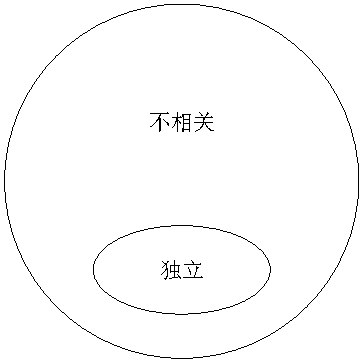
\includegraphics{fig3-4-1.pdf}
				\caption{不相关与独立的逻辑关系}\label{fig:3.4.1}
			\end{figure}

			另外可以看出, 前而有关数学期望的性质~\ref{pro:3.4.2}~:若 $X$ 与 $Y$ 相互独立, 则 $E(XY)=E(X)E(Y)$ , 现可以将条件“独立”降弱为“不相关”.

			协方差概念的引人可以完善随机变量和的方差计算, 请看下面性质.
		\end{proof}
	\end{property}
	\begin{property}\label{pro:3.4.6}
		对任意二维随机变量 $(X,Y)$ , 有
		\begin{equation}\label{eq:3.4.8}
			\Var(X \pm Y)=\Var(X)+\Var(Y)+2 \Cov(X, Y)
		\end{equation}
		\begin{proof}
			由方差的定义知
			\begin{align*}
				\Var(X \pm Y)&=E\{(X \pm Y)-E(X \pm Y)\}^{2} \\
				&=E\{(X-E(X)) \pm(Y-E(Y))\}^{2} \\
				&=E\left\{(X-E(X))^{2}+(Y-E(Y))^{2} \pm 2(X-E(X))(Y-E(Y))\right\} \\
			  &=\Var(X)+\Var(Y) \pm 2 \Cov(X, Y)
			\end{align*}
		\end{proof}
	\end{property}
	这个性质表明: 在 $X$ 与 $Y$ 相关的场合, 和的方差不等于方差的和. 或换句话说, 在 $X$ 与 $Y$ 不相关的场合, 和的方差等于方差的和. 这又可将前面有关方差的性质~\ref{pro:3.4.3}~:
	\begin{center}
		若 $X$ 与 $Y$ 相互独立, 则 $\Var(X \pm Y)=\Var(X)+\Var(Y)$
	\end{center}
	中的条件“独立”降弱为“不相关”.

	以上性质~\ref{pro:3.4.6}~还可以推广到更多个随机变量场合, 即对任意 $n$ 个随机变量 $X_1,X_2,\ldots,X_n$ , 有
	\begin{equation}\label{eq:3.4.9}
		\Var\left(\sum_{i=1}^{n} X_{i}\right)=\sum_{i=1}^{n} \Var\left(X_{i}\right)+2 \sum_{i=1}^{n} \sum_{j=1}^{i-1} \Cov\left(X_{i}, X_{j}\right).
	\end{equation}
	关于协方差的计算, 还有下面四条有用的性质.
	\begin{property}\label{pro:3.4.7}
		协方差 $\Cov(X,Y)$ 的计算与 $X,Y$ 的次序无关, 即
		\begin{equation*}
			\Cov(X,Y)=\Cov(Y,X).
		\end{equation*}
		\begin{proof}
			这由协方差的定义就可看出.
		\end{proof}
	\end{property}
	\begin{property}\label{pro:3.4.8}
		任意随机变量 $X$ 与常数 $a$ 的协方差为零, 即
		\begin{equation*}
			\Cov(X,a)=0.
		\end{equation*}
		\begin{proof}
			这只要用协方差的定义计算一下即可得知.
		\end{proof}
	\end{property}
	\begin{property}\label{pro:3.4.9}
		对任意常数 $a,b$ ,有
		\begin{equation*}
			\Cov(a X, b Y)=a b \Cov(X, Y).
		\end{equation*}
		\begin{proof}
			由协方差的定义知
			\begin{equation*}
				\Cov(a X, b Y)=E\{(a X-E(a X))(b Y-E(b Y)) \}
			\end{equation*}
			把公因子 $a$ 与 $b$ 提出, 即得 $ab\Cov(X,Y)$ .
		\end{proof}
	\end{property}
	\begin{property}\label{pro:3.4.10}
		设 $X,Y,Z$ 是任意三个随机变量, 则
		\begin{equation*}
			\Cov(X+Y, Z)=\Cov(X, Z)+\Cov(Y, Z)
		\end{equation*}
		\begin{proof}
			由协方差的性质~\ref{pro:3.4.4}~得
			\begin{align*}
				\Cov(X+Y, Z) &=E[(X+Y) Z]-E(X+Y) E(Z) \\
				&=E(X Z)+E(Y Z)-E(X) E(Z)-E(Y) E(Z) \\
				&=[E(X Z)-E(X) E(Z)]+[E(Y Z)-E(Y) E(Z)] \\
				&=\Cov(X, Z)+\Cov(Y, Z).
			\end{align*}
		\end{proof}
	\end{property}
	\begin{example}\label{exam:3.4.7}
		设二维随机变量 $(X,Y)$ 的联合密度函数为
		\begin{equation*}
			p(x,y)=\begin{cases}
				3x, & 0<y<x<1, \\
				0, & \text{其他}.
			\end{cases}
		\end{equation*}
		试求 $\Cov(X, Y)$ .
		\begin{proof}
			利用协方差的计算公式, 我们需要先计算 $E(X),E(Y),E(XY)$ 的值, 它们可直接用 $p(x,y)$ 导出, 但要注意积分限的确定, 具体如下.
			\begin{align*}
				&E(X)=\int_{0}^{1} \int_{0}^{x} x \cdot 3 x \dd y \dd x=\int_{0}^{1} 3 x^{3} \dd x=\frac{3}{4} \\
				&E(Y)=\int_{0}^{1} \int_{0}^{x} y \cdot 3 x \dd y \dd x=\int_{0}^{1} \frac{3 x^{3}}{2} \dd x=\frac{3}{8} \\
				&E(X Y)=\int_{0}^{1} \int_{0}^{x} x y \cdot 3 x \dd y \dd x=\int_{0}^{1} \frac{3 x^{4}}{2} \dd x=\frac{3}{10}.
			\end{align*}
			因此我们得
			\begin{equation*}
				\Cov(X, Y)=\frac{3}{10}-\frac{3}{4} \times \frac{3}{8}=\frac{3}{160}>0
			\end{equation*}
		\end{proof}
		由此我们还可以得结论: $X$ 与 $Y$ 不相互独立.
	\end{example}
	\begin{example}\label{exam:3.4.8}
		设二维随机变量 $(X,Y)$ 的联合密度函数为
		\begin{equation*}
			p(x,y)=\begin{cases}
				\frac{1}{3}(x+y), & 0<x<1,0<y<2; \\
				0, & \text{其他}.
			\end{cases}
		\end{equation*}
		试求 $\Var(2 X-3 Y+8)$ .
		\begin{solution}
			因为
			\begin{align*}
				\Var(2X-3Y+8)&=\Var(2X)+\Var(3Y)-2\Cov(2X,3Y) \\
				&=4\Var(X)+9\Var(Y)-12\Cov(X,Y).
			\end{align*}
		\end{solution}
		所以我们先分别计算 $E(X),E(Y),E\left( X^2 \right),E\left( Y^2 \right),E(XY)$ .为此先计算两个边际密度函数.
		\begin{align*}
			&p_{X}(x)=\int_{0}^{2} \frac{1}{3}(x+y) \dd y=\frac{2}{3}(x+1),  0<x<1\\
			&p_{Y}(y)=\int_{0}^{1} \frac{1}{3}(x+y) \dd x=\frac{1}{3}\left(\frac{1}{2}+y\right), 0<y<2
		\end{align*}
		然后再计算一、二阶矩,
		\begin{align*}
			&E(X)=\int_{0}^{1} \frac{2}{3} x(x+1) \dd x=\frac{5}{9}.\\
			&E\left( X^2 \right)=\int_{0}^{1} \frac{2}{3} x^{2}(x+1) \dd x=\frac{7}{8}.\\
			&E(Y)=\int_{0}^{2} \frac{1}{3} y\left(\frac{1}{2}+y\right) \dd y=\frac{11}{9}.\\
			&E\left( Y^2 \right)=\int_{0}^{2} \frac{1}{3} y^{2}\left(\frac{1}{2}+y\right) \dd y=\frac{16}{9}.
		\end{align*}
		由此可得
		\begin{equation*}
			\Var(X)=\frac{7}{8}-\left(\frac{5}{9}\right)^{2}=\frac{13}{162},\quad \Var(Y)=\frac{16}{9}-\left(\frac{11}{9}\right)^{2}=\frac{23}{81}.
		\end{equation*}
		最后还需要计算 $E(XY)$ , 它只能从联合密度函数导出.
		\begin{equation*}
			E(X Y)=\frac{1}{3} \int_{0}^{1} \int_{0}^{2} x y(x+y) \dd y \dd x=\frac{1}{3} \int_{0}^{1}\left(2 x^{2}+\frac{8}{3} x\right) \dd x=\frac{2}{3}.
		\end{equation*}
		于是得协方差为
		\begin{equation*}
			\Cov(X, Y)=\frac{2}{3}-\frac{5}{9} \times \frac{11}{9}=-\frac{1}{81}.
		\end{equation*}
		代回原式得
		\begin{equation*}
			\Var(2 X-3 Y+8)=4 \times \frac{13}{162}+9 \times \frac{23}{81}-12 \times\left(-\frac{1}{81}\right)=\frac{245}{81}.
		\end{equation*}
	\end{example}
	\subsection{相关系数}\label{ssec:3.4.4}
	协方差 $\Cov(X, Y)$ 是有量纲的量, 譬如 $X$ 表示人的身高, 单位是米 $(\mathrm{m})$ , $Y$ 表示人的体重, 单位是公斤 $(\mathrm{kg})$ , 则 $\Cov(X, Y)$ 带有量纲 $(\mathrm{m\cdot kg})$ . 为了消除量纲的影响, 现对协方差除以相同量纲的量, 就得到一个新的概念——相关系数, 它的定义如下.
	\begin{definition}{}{3.4.2}
		设 $(X,Y)$ 是一个二维随机变量, 且 $\Var(X)>0,\Var(Y)>0$ . 则称
		\begin{equation}\label{eq:3.4.10}
			\Corr(X, Y)=\frac{\Cov(X, Y)}{\sqrt{\Var(X)}\sqrt{\Var(Y)}}=\frac{\Cov(X, Y)}{\sigma_{X} \sigma_{Y}}
		\end{equation}
		为 $X$ 与 $Y$ 的(线性)\textbf{相关系数}.
	\end{definition}
	从以上定义中可看出: 相关系数 $\Corr(X, Y)$ 与协方差 $\Cov(X, Y)$ 是同符号的, 即同为正, 或同为负, 或同为零. 这说明, 从相关系数的取值也可反映出 $X$ 与 $Y$ 的正相关、负相关和不相关.

	相关系数的另一个解释是: 它是相应标准化变量的协方差. 若记 $X$ 与 $Y$ 的数学期望分别为 $\mu_{X},\mu_{Y}$ , 其标准化变量为
	\begin{equation*}
		X^{*}=\frac{X-\mu_{X}}{\sigma_{X}},\quad Y^{*}=\frac{Y-\mu_{Y}}{\sigma_{Y}},
	\end{equation*}
	则有
	\begin{equation*}
		\Cov\left(X^{*}, Y^{*}\right)=\Cov\left(\frac{X-\mu_{X}}{\sigma_{X}}, \frac{Y-\mu_{Y}}{\sigma_{Y}}\right)=\frac{\Cov(X, Y)}{\sigma_{X}\sigma_{Y}}=\Corr(X, Y)
	\end{equation*}
	\begin{example}\label{exam:3.4.9}
		二维正态分布 $N\left(\mu_{1}, \mu_{2}, \sigma_{1}^{2}, \sigma_{2}^{2}, \rho\right)$ 的相关系数就是 $\rho$ .
		\begin{solution}
			下面先求 $\Cov(X,Y)$ .
			\begin{align*}
				\Cov(X,Y)&=E[ (X-E(X)) (Y-E(Y)) ]\\
				&=\frac{1}{2\uppi \sigma_1\sigma_2\sqrt{1-\rho^2}} \int_{-\infty}^{+\infty}\int_{-\infty}^{+\infty} (x-\mu_1)(y-\mu_2) \cdot \\
				&\quad\exp\left\{ -\frac{1}{2\left( 1-\rho^2 \right)  }\left[ \frac{(x-\mu_1)^2}{\sigma_1^2}-2\rho\frac{(x-\mu_1)(y-\mu_2)}{\sigma_1\sigma_2}+\frac{(y-\mu_2)^2}{\sigma_2^2} \right] \right\}\dd x \dd y.
			\end{align*}
			先将上式中方括号化成
			\begin{equation*}
				\left( \frac{(x-\mu_1)}{\sigma_1}-\rho\frac{y-\mu_2}{\sigma_2} \right)^2+\left( \sqrt{1-\rho^2}\frac{y-\mu_2}{\sigma_2} \right)^2,
			\end{equation*}
			再作变量变换
			\begin{equation*}
				\begin{cases}
					u=\frac{1}{\sqrt{1-\rho^2}}\left( \frac{x-\mu_1}{\sigma_1}-\rho\frac{y-\mu_2}{\sigma_2} \right),\\
					v=\frac{y-\mu_2}{\sigma_2},
				\end{cases}
			\end{equation*}
			则
			\begin{equation*}
				\begin{cases}
					x-\mu_1=\sigma_1\left[ u\sqrt{1-\rho^2}+\rho v \right],\\
					y-\mu_2=\sigma_2 v,
				\end{cases}
			\end{equation*}
			\begin{equation*}
				\dd x\dd y=\sigma_1 \sigma_2 \sqrt{1-\rho^2}\dd u\dd v.
			\end{equation*}
			由此得
			\begin{equation*}
				\Cov(X,Y)=\frac{\sigma_1\sigma_2}{2\uppi}\int_{-\infty}^{+\infty}\int_{-\infty}^{+\infty}\left[ uv\sqrt{1-\rho^2}+\rho v^2 \right]\exp\left\{ -\frac{1}{2}\left( u^2+v^2 \right) \right\}\dd u\dd v.
			\end{equation*}
			上式右端积分可以分为两个积分, 其中
			\begin{align*}
				&\int_{-\infty}^{+\infty}\int_{-\infty}^{+\infty} uv\exp\left\{ -\frac{1}{2}\left( u^2+v^2 \right) \right\}\dd u\dd v=0,\\
				&\int_{-\infty}^{+\infty}\int_{-\infty}^{+\infty} v^2\exp\left\{ -\frac{1}{2}\left( u^2+v^2 \right) \right\}\dd u\dd v=2\uppi.
			\end{align*}
			从而
			\begin{equation*}
				\Cov(X,Y)=\frac{\sigma_1\sigma_2}{2\uppi}\cdot \rho\cdot 2\uppi=\rho\sigma_1\sigma_2,
			\end{equation*}
			\begin{equation*}
				\Corr(X,Y)=\frac{\Cov(X,Y)}{\sigma_1\sigma_2}=\rho.
			\end{equation*}
		\end{solution}
	\end{example}
	为了研究相关系数的性质, 需要如下引理.
	\begin{lemma}{施瓦茨不等式}{3.4.1}
		对任意二维随机变量 $(X,Y)$ , 若 $X$ 与 $Y$ 的方差都存在, 且记 $\sigma_{X}^2=\Var(X),\sigma_{Y}^2=\Var(Y)$ , 则有
		\begin{equation}\label{eq:3.4.11}
			[\Cov(X,Y)]^2\leq \sigma_{X}^2\sigma_{Y}^2.
		\end{equation}
		\begin{proof}
			不妨设 $\sigma_{X}^2>0$ , 因为当 $\sigma_{X}^2=0$ 时, 则 $X$ 几乎处处为常数, 因而其与 $Y$ 的协方差亦为零, 从而~\eqref{eq:3.4.11}~式两端皆为零, 结论成立. 在 $\sigma_{X}^2>0$ 成立下, 考虑 $t$ 的如下二次函数:
			\begin{equation*}
				g(t)=E[t(X-E(X))+(Y-E(Y))]^2=t^2 \sigma_{X}^2+2t\cdot \Cov(X,Y)+\sigma_{Y}^2.
			\end{equation*}
			由于上述的二次三项式非负, 平方项系数 $\sigma_{X}^2$ 为正, 所以其判别式小于或等于零, 即
			\begin{equation*}
				[2\Cov(X,Y)]^2-4\sigma_{X}^2\sigma_{Y}^2\leq0.
			\end{equation*}
			移项后即得施瓦茨不等式.
		\end{proof}
		利用施瓦茨不等式立即可得相关系数的一个重要性质.
	\end{lemma}
	\begin{property}\label{pro:3.4.11}
		$-1\leq\Corr(X,Y)\leq1$ .

		这个性质表明: 相关系数介于 $-1$ 与 $1$ 之间. 对相关系数为 $\pm 1$ 时, 有另一重要性质.
	\end{property}
	\begin{property}\label{pro:3.4.12}
		$\Corr(X,Y)=\pm 1$ 的充要条件是 $X$ 与 $Y$ 间几乎处处有线性关系, 即存在 $a(\ne0)$ 与 $b$ , 使得
		\begin{equation*}
			P(Y=aX+b)=1.
		\end{equation*}
		其中当 $\Corr(X,Y)=1$ 时, 有 $a>0$ ; 当 $\Corr(X,Y)=-1$ 时, 有 $a<0$ .
		\begin{proof}
			充分性. 若 $Y=aX+b(X=cY+d\text{也一样})$ , 则将
			\begin{equation*}
				\Var(Y)=a^2\Var(X),\Cov(X,Y)=a\Cov(X,X)=a\Var(X)
			\end{equation*}
			代入相关系数的定义中得
			\begin{equation*}
				\Corr(X,Y)=\frac{\Cov(X,Y)}{\sigma_{X}\sigma_{Y}}=\frac{a\Var(X)}{|a|\Var(X)}=\begin{cases}
					1, & a>0;\\
					-1, & a<0.
				\end{cases}
			\end{equation*}
			必要性. 因为
			\begin{equation}\label{eq:3.4.12}
				\Var\left( \frac{X}{\sigma_{X}}\pm\frac{Y}{\sigma_{Y}} \right)=2[1\pm\Corr(X,Y)],
			\end{equation}
			所以当 $\Corr(X,Y)=1$ 时, 有
			\begin{equation*}
				\Var\left( \frac{X}{\sigma_{X}}-\frac{Y}{\sigma_{Y}} \right)=0,
			\end{equation*}
			由此得
			\begin{equation*}
				P\left( \frac{X}{\sigma_{X}}-\frac{Y}{\sigma_{Y}}=c \right)=1,
			\end{equation*}
			或
			\begin{equation*}
				P\left( Y=\frac{\sigma_{Y}}{\sigma_{X}}X-c\sigma_{Y} \right)=1.
			\end{equation*}
			这就证明了: 当 $\Corr(X,Y)=1$ 时, $Y$ 与 $X$ 几乎处处线性正相关.

			当 $\Corr(X,Y)=-1$ 时, 由 $\eqref{eq:3.4.12}$ 得
			\begin{equation*}
				\Var\left( \frac{X}{\sigma_{X}}+\frac{Y}{\sigma_{Y}} \right)=0,
			\end{equation*}
			由此得
			\begin{equation*}
				P\left( \frac{X}{\sigma_{X}}+\frac{Y}{\sigma_{Y}}=c \right)=1,
			\end{equation*}
			或
			\begin{equation*}
				P\left( Y=-\frac{\sigma_{Y}}{\sigma_{X}}X+c\sigma_{Y} \right)=1.
			\end{equation*}
			这也证明了: 当 $\Corr(X,Y)=-1$ 时, $Y$ 与 $X$ 几乎处处线性负相关.
		\end{proof}
	\end{property}
	对于这个性质可作以下几点说明:
	\begin{itemize}
			\item 相关系数 $\Corr(X,Y)$ 刻画了 $X$ 与 $Y$ 之间的线性关系, 因此也常称其为“线性相关系数”.
			\item 若 $\Corr(X,Y)=0$ , 则称 $X$ 与 $Y$ 不相关. 不相关是指 $X$ 与 $Y$ 之间没有线性关系, 但 $X$ 与 $Y$ 之间可能有其他的函数关系, 譬如平方关系、对数关系等.
			\item 若 $\Corr(X,Y)=1$ , 则称 $X$ 与 $Y$ 完全正相关; 若 $\Corr(X,Y)=-1$ , 则称 $X$ 与 $Y$ 完全负相关.
			\item 若 $0<|\Corr(X,Y)|<1$ , 则称 $X$ 与 $Y$ 有“一定程度”的线性关系. $|\Corr(X,Y)|$ 越接近于 $1$ , 则线性相关程度越高; $|\Corr(X,Y)|$ 越接近于 $0$ , 则线性相关程度越低. 而协方差看不出这一点. 若协方差很小, 而其两个标准差 $\sigma_{X}$ 和 $\sigma_{Y}$ 也很小, 则其比值就不一定很小, 这可从下面例~\ref{exam:3.4.10}~看出.
	\end{itemize}
	\begin{example}\label{exam:3.4.10}
		已知随机向量 $(X,Y)$ 的联合密度函数为
		\begin{equation*}
			p(x,y)=\begin{cases}
				\frac{8}{3}, & 0<x-y<0.5,0<x,y<1;\\
				0, & \text{其他}.
			\end{cases}
		\end{equation*}
		求 $X,Y$ 的相关系数 $\Corr(X,Y)$ .
		\begin{solution}
			先计算两个边际密度函数.

			当 $0<x<0.5$ 时,
			\begin{equation*}
				p_{X}(x)=\int_{-\infty}^{+\infty}p(x,y)\dd y=\int_{0}^{x}\frac{8}{3}\dd y=\frac{8}{3}x,
			\end{equation*}
			当 $0.5<x<1$ 时,
			\begin{equation*}
				p_{X}(x)=\int_{-\infty}^{+\infty}p(x,y)\dd y=\int_{x-0.5}^{x}\frac{8}{3}\dd y=\frac{4}{3},
			\end{equation*}
			\begin{figure}[htbp]
				\centering
				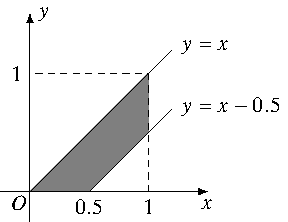
\includegraphics{fig3-4-2}
				\caption{例~\ref{exam:3.4.10}~中 $p(x,y)$ 的非零区域}\label{fig:3.4.2}
			\end{figure}
			所以得 $X$ 的边际密度函数为
			\begin{equation*}
				p_{X}(x)=\begin{cases}
					\frac{8}{3}x, & 0<x<0.5;\\
					\frac{4}{3}, & 0.5<x<1;\\
					0, & \text{其他}.
				\end{cases}
			\end{equation*}
			当 $0<y<0.5$ 时,
			\begin{equation*}
				p_{Y}(y)=\int_{-\infty}^{+\infty} p(x, y) \dd x=\int_{y}^{y+0.5} \frac{8}{3} \dd x=\frac{4}{3};
			\end{equation*}
			当 $0.5<y<1$ 时,
			\begin{equation*}
				p_{Y}(y)=\int_{-\infty}^{+\infty} p(x, y) \dd x=\int_{y}^{1} \frac{8}{3} \dd x=\frac{8}{3}(1-y).
			\end{equation*}
			所以得 $Y$ 的边际密度函数为
			\begin{equation*}
				p_{Y}(y)=\begin{cases}
					\frac{4}{3}, & 0<x<0.5;\\
					\frac{8}{3}(1-y), & 0.5<x<1;\\
					0, & \text{其他}.
				\end{cases}
			\end{equation*}
			然后分别计算 $X$ 与 $Y$ 的一、二阶矩
			\begin{align*}
				&E(X)=\int_{0}^{0.5} \frac{8}{3} x^{2} \dd x+\int_{0.5}^{1} \frac{4}{3} x \dd x=\frac{11}{18},\\
				&E(Y)=\int_{0}^{0.5} \frac{4}{3} y \dd y+\int_{0.5}^{1} \frac{8}{3} y(1-y) \dd y=\frac{7}{18},\\
				&E\left(X^{2}\right)=\int_{0}^{0.5} \frac{8}{3} x^{3} \dd x+\int_{0.5}^{1} \frac{4}{3} x^{2} \dd x=\frac{31}{72},\\
				&E\left(Y^{2}\right)=\int_{0}^{0.5} \frac{4}{3} y^{2} \dd y+\int_{0.5}^{1} \frac{8}{3} y^{2}(1-y) \dd y=\frac{15}{72}.
			\end{align*}
			由此可得 $X$ 与 $Y$ 各自的方差
			\begin{align*}
				&\Var(X)=\frac{31}{72}-\left(\frac{11}{18}\right)=\frac{37}{648},\\
				&\Var(Y)=\frac{15}{72}-\left(\frac{7}{18}\right)^{2}=\frac{37}{648}
			\end{align*}
			最后还需要计算 $E(XY)$ , 它只能从联合密度函数导出.
			\begin{align*}
				E(XY)&=\int_{0}^{0.5} \int_{0}^{x} \frac{8}{3} x y \dd y \dd x+\int_{0.5}^{1} \int_{x-0.5}^{x} \frac{8}{3} x y \dd y \dd x\\
				&=\int_{0}^{0.5} \frac{4}{3} x^{3} \dd x+\int_{0.5}^{1} \frac{4}{3} x\left(x-\frac{1}{4}\right) \dd x=\frac{1}{48}+\frac{7}{18}-\frac{1}{8}=\frac{41}{144}
			\end{align*}
			最后得协方差和相关系数为
			\begin{align*}
				&\Cov(X,Y)=\frac{41}{144}-\frac{11}{18} \times \frac{7}{18}=\frac{61}{1296}=0.0471.\\
				&\Corr(X,Y)=\frac{\Cov(X,Y)}{\sigma_{X}\sigma_{Y}}=\frac{61}{1296} \times \frac{648}{37}=\frac{61}{74}=0.8243.
			\end{align*}
			这个协方差很小, 但其相关系数并不小.
		\end{solution}
	\end{example}
	上例中, 从相关系数 $\Corr(X,Y)=0.8243$ 看, $X$ 与 $Y$ 有相当程度的正相关; 但从相应的协方差 $\Cov(X,Y)=0.0471$ 看, $X$ 与 $Y$ 的相关性很微弱, 几乎可以忽略不计. 造成这种错觉的原因在于没有考虑标准差, 若两个标准差都很小, 即使协方差小一些, 相关系数也能显示一定程度的相关性. 由此可见, 在协方差的基础上加工形成的相关系数是更为重要的相关性的特征数.

	在一般场合, 独立必导致不相关, 但不相关推不出独立. 但也有例外, 下面的性质指出了这个例外.
	\begin{property}\label{pro:3.4.13}
		在二维正态分布 $N(\mu_1,\mu_2,\sigma_1^2,\sigma_2^2,\rho)$ 的相关系数是 $\rho$ , 因此我们只需证 $\rho=0$ 与独立是等价的. 因为二维正态分布 $N(\mu_1,\mu_2,\sigma_1^2,\sigma_2^2,\rho)$ 的两个边际分布为 $N(\mu_1,\sigma_1^2)$ 和 $N(\mu_2,\sigma_2^2)$ , 所以记其联合密度函数为 $p(x,y)$ , 边际密度函数为 $p_{X}(x)$ 与 $p_{Y}(y)$ .

		当 $\rho=0$ 时, 可从正态密度函数的表达式中看出
		\begin{equation*}
			p(x,y)=p_{X}(x)p_{Y}(y),
		\end{equation*}
		即 $X$ 与 $Y$ 相互独立.

		反之, 若 $X$ 与 $Y$ 相互独立, 即对一切 $x$ 与 $y$ 有 $p(x,y)=p_{X}(x)p_{Y}(y)$ , 若令 $x=\mu_1,y=\mu_2$ , 则可得
		\begin{equation*}
			\frac{1}{\sqrt{1-\rho^2}}=1,
		\end{equation*}
		从而有 $\rho=0$ . 结论得证.
	\end{property}
	\begin{example}[(投资风险组合)]\label{exam:3.4.11}
		设有一笔资金, 总量记为 $1$ (可以是 $1$ 万元, 也可以是 $100$ 万元等), 如今要投资甲、乙两种证券. 若将资金 $x_1$ 投资于甲证券, 将余下的资金 $1-x_1=x_2$ 投资于乙证券, 于是 $(x_1,x_2)$ 就形成了一个投资组合. 记 $X$ 为投资甲证券的收益率, $Y$ 为投资乙证券的收益率, 它们都是随机变量. 如果已知 $X$ 和 $Y$ 的均值(代表平均收益)分别为 $\mu_1$ 和 $\mu_2$ , 方差(代表风险)分别为 $\sigma_1^2$ 和 $\sigma_2^2$ , $X$ 和 $Y$ 间的相关系数为 $\rho$ . 试求该投资组合的平均收益与风险(方差), 并求使投资风险最小的 $x_1$ 是多少?
		\begin{solution}
			因为组合收益为
			\begin{equation*}
				Z=x_{1} X+x_{2} Y=x_{1} X+\left(1-x_{1}\right) Y,
			\end{equation*}
			所以该组合的平均收益为
			\begin{equation*}
				E(Z)=x_{1} E(X)+\left(1-x_{1}\right) E(Y)=x_{1} \mu_{1}+\left(1-x_{1}\right) \mu_{2}.
			\end{equation*}
			而该组合的风险(方差)为
			\begin{align*}
				\Var(Z)&=\Var\{ x_1 X+(1-x_1)Y \}\\
				&=x_{1}^{2} \Var(X)+\left(1-x_{1}\right)^{2} \Var(Y)+2 x_{1}\left(1-x_{1}\right) \Cov(X, Y)\\
				&=x_{1}^{2} \sigma_{1}^{2}+\left(1-x_{1}\right)^{2} \sigma_{2}^{2}+2 x_{1}\left(1-x_{1}\right) \rho \sigma_{1} \sigma_{2}.
			\end{align*}
			求最小组合风险, 即求 $\Var(Z)$ 关于 $x_1$ 的极小点, 为此令
			\begin{equation*}
				\frac{\dd(\Var(Z))}{\dd x_{1}}=2 x_{1} \sigma_{1}^{2}-2\left(1-x_{1}\right) \sigma_{2}^{2}+2 \rho \sigma_{1} \sigma_{2}-4 x_{1} \rho \sigma_{1} \sigma_{2}=0.
			\end{equation*}
			从中解得
			\begin{equation*}
				x_1^{*}=\frac{\sigma_{2}^{2}-\rho \sigma_{1} \sigma_{2}}{\sigma_{1}^{2}+\sigma_{2}^{2}-2 \rho \sigma_{1} \sigma_{2}}.
			\end{equation*}
			它与 $\mu_1,\mu_2$ 无关. 又因为 $\Var(Z)$ 中 $x_1^2$ 的系数为正, 所以以上的 $x_1^{*}$ 可使组合风险达到最小.
		\end{solution}
		譬如, $\sigma_{1}^{2}=0.3, \sigma_{2}^{2}=0.5, \rho=0.4$ , 则
		\begin{equation*}
			x_{1}^{*}=\frac{0.5-0.4 \sqrt{0.3 \times 0.5}}{0.3+0.5-2 \times 0.4 \sqrt{0.3 \times 0.5}}=0.704
		\end{equation*}
		这说明应把全部资金的 $70\%$ 投资于甲证券, 而把余下的 $30\%$ 资金投向乙证券,这样的投资组合风险最小.
	\end{example}
	\subsection{随机向量的数学期望与协方差阵}\label{ssec:3.4.5}
	以下我们用矩阵形式给出 $n$ 维随机变量的数学期望与方差.
	\begin{definition}{}{3.4.3}
		记 $n$ 维随机向量为 $\boldsymbol{X}=(X_1,X_2,\ldots,X_n)'$ , 若其每个分量的数学期望都存在, 则称
		\begin{equation*}
			E(\boldsymbol{X})=(E(X_1),E(X_2),\ldots,E(X_n))'
		\end{equation*}
		为 $n$ 维随机向量 $\boldsymbol{X}$ 的\textbf{数学期望向量}, 简称为 $\boldsymbol{X}$ 的\textbf{数学期望}, 而称
		\begin{align*}
			&E[ (\boldsymbol{X}-E(\boldsymbol{X})) (\boldsymbol{X}-E(\boldsymbol{X}))' ]\\
			&=\begin{pmatrix}
				\Var(X_1) & \Cov(X_1,X_2) & \cdots & \Cov(X_1,X_n)\\
				\Cov(X_2,X_1) & \Var(X_2) & \cdots & \Cov(X_2,X_n)\\
				\vdots & \vdots & &\vdots\\
				\Cov(X_n,X_1) & \Cov(X_n,X_2) & \cdots & \Var(X_n)
			\end{pmatrix}
		\end{align*}
		为该随机向量的\textbf{方差—协方差阵}, 简称\textbf{协方差阵}, 记为 $\Cov(\boldsymbol{X})$ .
	\end{definition}
	至此我们可以看出, $n$ 维随机向量的数学期望是各分量的数学期望组成的向量. 而其方差就是由各分量的方差与协方差组成的矩阵, 其对角线上的元素就是方差, 非对角线元素为协方差.

	以下给出的协方差阵的一个重要性质.
	\begin{theorem}{}{3.4.2}
		$n$ 维随机向量的协方差阵 $\Cov(\boldsymbol{X})=( \Cov\left(X_i,X_j\right) )_{n\times n}$ 是一个对称的非负定矩阵.
		\begin{proof}
			因为 $\Cov\left(X_i,X_j\right)=\Cov\left(X_j,X_i\right)$ , 所以对称性是显然的. 下证非负定性. 因为对任意的 $n$ 维实向量 $\boldsymbol{c}=(c_1,c_2,\ldots,c_n)'$ , 有
			\begin{align*}
				\boldsymbol{c}'\Cov(\boldsymbol{X})\boldsymbol{c} &= (c_1,c_2,\ldots,c_n)\begin{pmatrix}
					\Var(X_1) & \cdots & \Cov(X_1,X_n)\\
					\Cov(X_2,X_1) & \cdots & \Cov(X_2,X_n)\\
					\vdots & & \vdots\\
					\Cov(X_n,X_1) & \cdots & \Var(X_n)
				\end{pmatrix}
				\begin{pmatrix}
					c_1\\
					c_2\\
					\vdots\\
					c_n
				\end{pmatrix}\\
				&= \sum_{i=1}^{n}\sum_{j=1}^{n}c_{i}c_{j}\Cov(X_i,X_j)\\
				&= \sum_{i=1}^{n}\sum_{j=1}^{n}E\{ [c_{i} (X_{i}-E(X_{i}))] [c_{j}(X_{j}-E(X_{j}))] \}\\
				&= E\left\{\sum_{i=1}^{n} \sum_{j=1}^{n}\left[c_{i}\left(X_{i}-E\left(X_{i}\right)\right)\right]\left[c_{j}\left(X_{j}-E\left(X_{j}\right)\right)\right]\right\}\\
				&= E\left\{\left[\sum_{i=1}^{n} c_{i}\left(X_{i}-E\left(X_{i}\right)\right)\right]\left[\sum_{j=1}^{n} c_{j}\left(X_{j}-E\left(X_{j}\right)\right)\right]\right\}\\
				&= E\left[\sum_{i=1}^{n} c_{i}\left(X_{i}-E\left(X_{i}\right)\right)\right]^{2} \geqslant 0
			\end{align*}
			所以矩阵 $\Cov(\boldsymbol{X})$ 是非负定的, 定理得证.
		\end{proof}
	\end{theorem}
	\begin{example}[( $n$ 元正态分布)]\label{exam:3.4.12}
		设 $n$ 维随机变量 $\boldsymbol{X}=(X_1,X_2,\ldots,X_n)'$ 的协方阵为 $\boldsymbol{B}=\Cov(\boldsymbol{X})$ , 数学期望向量为 $\boldsymbol{a}=(a_1,a_2,\ldots,a_n)'$ . 又记 $\boldsymbol{x}=(x_1,x_2,\ldots,x_n)'$ , 则由密度函数
		\begin{equation}\label{eq:3.4.13}
			p(x_1,x_2,\ldots,x_n)=p(\boldsymbol{x})=\frac{1}{ (2\uppi)^{\frac{n}{2}} |\boldsymbol{B}|^{\frac{1}{2}} }\exp\left\{ -\frac{1}{2}(\boldsymbol{x}-\boldsymbol{a})'\boldsymbol{B}^{-1}(\boldsymbol{x}-\boldsymbol{a}) \right\}
		\end{equation}
		定义的分布称为 $n$ 元正态分布, 记为 $\boldsymbol{X}\sim N(\boldsymbol{a},\boldsymbol{B})$ . 其中 $|\boldsymbol{B}|$ 表示 $\boldsymbol{B}$ 的行列式, $\boldsymbol{B}^{-1}$ 表示 $\boldsymbol{B}$ 的逆阵, $(\boldsymbol{x}-\boldsymbol{a})'$ 表示向量 $(\boldsymbol{x}-\boldsymbol{a})$ 的转置.

		若记 $\boldsymbol{B}^{-1}=(r_{ij})$ , 则~\eqref{eq:3.4.13}~式可写成
		\begin{equation}\label{eq:3.4.14}
			p\left(x_{1}, x_{2}, \ldots, x_{n}\right)=\frac{1}{ (2\uppi)^{\frac{n}{2}} |\boldsymbol{B}|^{\frac{1}{2}} }\exp\left\{ -\frac{1}{2}\sum_{i,j=1}^{n}r_{ij}(x_{i}-a_{i})(x_{j}-a_{j}) \right\}.
		\end{equation}
		若取数学期望向量和协方差矩阵分别为
		\begin{equation*}
			\boldsymbol{a}=\begin{pmatrix}
				\mu_1\\
				\mu_2
			\end{pmatrix},\quad \boldsymbol{B}=\begin{pmatrix}
				\sigma_1^2 & \sigma_1\sigma_2\rho\\
				\sigma_1\sigma_2\rho & \sigma_2^2
			\end{pmatrix},
		\end{equation*}
		代入~\eqref{eq:3.4.13}~式, 则可得到~\eqref{eq:3.1.8}~式给出的二元正态密度函数.

		$n$ 元正态分布是一种最重要的多维分布, 它在概率论、数理统计和随机过程中都占有重要地位.
	\end{example}
	\begin{xiti}
		\item 掷一颗均匀的骰子 $2$ 次, 其最小点数记为 $X$ , 求 $E(X)$ .
		\item 求掷 $n$ 颗骰子出现点数之和的数学期望与方差.
		\item 从数字 $0,1,\ldots,n$ 中任取两个不同的数字, 求这两个数字之差的绝对值的数学期望.
		\item 设在区间 $(0,1)$ 上随机地取 $n$ 个点, 求相距最远的两点间的距离的数学期望.
		\item 盘中有 $n$ 个不同的球, 其上分别写有数字 $1,2,\ldots,n$ . 每次随机抽出一个, 记下其号码, 放回去再抽. 直到抽到有两个不同的数字为止. 求平均抽球次数.
		\item 设随机变量 $(X,Y)$ 的联合分布列为
			\begin{center}
				\begin{tabularx}{0.8\textwidth}{YYY}
					\toprule
					 & \multicolumn{2}{c}{$Y$}\\
					\cmidrule{2-3}
					X & 0 & 1\\
					\midrule
					0 & 0.1 & 0.15\\
					1 & 0.25 & 0.2\\
					2 & 0.15 & 0.15\\
					\bottomrule
				\end{tabularx}
			\end{center}
		试求 $Z=\sin\left[ \frac{\uppi}{2}(X+Y) \right]$ 的数学期望.
		\item 随机变量 $(X,Y)$ 服从以点 $(0,1),(1,0),(1,1)$ 为顶点的三角形区域上的均匀分布, 试求 $E(X+Y)$ 和 $\Var(X+Y)$ .
		\item 设随机变量 $(X,Y)$ 的联合密度函数为
			\begin{equation*}
				p(x,y)=\begin{cases}
					x(1+3y^2)/4, & 0<x<2,0<y<1;\\
					0, & \text{其他}.
				\end{cases}
			\end{equation*}
			试求 $E(Y/X)$ .
		\item 设 $X_1,X_2,\ldots,X_5$ 是独立同分布的随机变量, 其共同密度函数为
			\begin{equation*}
				p(x)=\begin{cases}
					2x, & 0<x<1;\\
					0, & \text{其他}.
				\end{cases}
			\end{equation*}
			试求 $Y=\max \left(X_{1}, X_{2}, \ldots, X_{5}\right)$ 的密度函数、数学期望和方差.
		\item 系统由 $n$ 个部件组成. 记 $X_i$ 为第 $i$ 个部件能持续工作的时间, 如果 $X_1,\ldots,X_n$ 独立同分布, 且 $X_i\sim Exp(\lambda)$ , 试在以下情况下求系统持续工作的平均时间:
			\begin{enumerate}
				\item 如果有一个部件停止工作, 系统就不工作了;
				\item 如果至少有一个部件在工作, 系统就工作.
			\end{enumerate}
		\item 邮局里有 $A$ 、 $B$ 、 $C$ 三个顾客, 假定邮局对每个顾客的服务时间服从参数为 $\lambda$ 的指数分布. 对 $A$ 和 $B$ 立即开始服务, 在对 $A$ 或 $B$ 结束服务后开始对 $C$ 服务, 对 $A$ 、 $B$ 两人服务所需的时间是独立的. 求 $C$ 在邮局中
			\begin{enumerate}
				\item 等待时间的数学期望;
				\item 逗留时间的数学期望.
			\end{enumerate}
		\item 设 $X,Y$ 独立同分布, 都服从标准正态分布 $N(0,1)$ , 求 $E[\max(X,Y)]$ .
		\item 设随机变量 $X_1,X_2,\ldots,X_n$ 相互独立, 且都服从 $(0,\theta)$ 上的均匀分布, 记
			\begin{equation*}
				Y=\max \left\{X_{1}, X_{2}, \ldots, X_{n}\right\},\quad Z=\min \left\{X_{1}, X_{2}, \ldots, X_{n}\right\}.
			\end{equation*}
			试求 $E(Y)$ 和 $E(Z)$ .
		\item 设随机变量 $U$ 服从 $(-2,2)$ 上的均匀分布, 定义 $X$ 和 $Y$ 如下:
			\begin{equation*}
				X=\begin{cases}
					-1, & \text{若}U<-1;\\
					1, & \text{若}U\geqslant -1.
				\end{cases}\quad
				Y=\begin{cases}
					-1, & \text{若}U<1;\\
					1, & \text{若}U\geqslant 1.
				\end{cases}
			\end{equation*}
			试求 $\Var(X+Y)$ .
		\item 一商店经销某种商品, 每周进货量 $X$ 与顾客对该种商品的需求量 $Y$ 是相互独立的随机变量, 且都跟从区间 $(10,20)$ 上的均匀分布. 商店每售出一单位商品可得利润 $1000$ 元; 若需求量超过了进货量, 则可从其他商店调剂供应, 这时每单位商品获利润为 $500$ 元. 试求此商店经销该种商品每局的平均利润.
		\item 设随机变量 $X$ 与 $Y$ 独立, 都服从正态分布 $N\left(a,\sigma^2\right)$ , 试证
			\begin{equation*}
				E[\max(X,Y)]=a+\frac{\sigma}{\sqrt{\uppi}}.
			\end{equation*}
		\item 设二维随机变量 $(X,Y)$ 的联合分布列为
			\begin{center}
				\begin{tabularx}{0.8\textwidth}{YYYY}
					\toprule
					 & \multicolumn{3}{c}{$Y$}\\
					\cmidrule{2-4}
					X & -1 & 0 & 1\\
					\midrule
					0 & 0.07 & 0.18 & 0.15\\
					1 & 0.08 & 0.32 & 0.20\\
					\bottomrule
				\end{tabularx}
			\end{center}
			试求 $X^2$ 与 $Y^2$ 的协方差.
			\item 把一个骰子独立地掷 $n$ 次, 求 $1$ 点出现的次数与 $6$ 点出现次数的协方差及相关系数.
			\item 某箱装 $100$ 件产品, 其中一、二和三等品分别为 $80$ , $10$ 和 $10$ 件. 现从中随机取一件, 定义三个随机变量 $X_1,X_2,X_3$ 如下
				\begin{equation*}
					X_i=\begin{cases}
						1, & \text{若抽到} i \text{等品};\\
						0, & \text{其他}.
					\end{cases}\quad
					i=1,2,3.
				\end{equation*}
				试求随机变量 $X_1$ 和 $X_2$ 的相关系数 $\Corr(X_1,X_2)$ .
			\item 将一枚硬币重复掷 $n$ 次, 以 $X$ 和 $Y$ 分别表示正面向上和反面向上的次数, 试求 $X$ 和 $Y$ 的协方差及相关系数.
			\item 设随机变量 $X$ 和 $Y$ 独立同服从参数为 $\lambda$ 的泊松分布, 令
				\begin{equation*}
					U=2X+Y,\quad V=2X-Y.
				\end{equation*}
				求 $U$ 和 $V$ 的相关系数 $\Corr(U,V)$ .
			\item 在一个有 $n$ 个人参加的晚会上, 每个人带了一件礼物, 且假定各人带的礼物都不相同. 晚会期间各人从放在一起的 $n$ 件礼物中随机抽取一件, 试求选中自己礼品的人数 $X$ 的均值和方差.
			\item 设随机变量 $X$ 和 $Y$ 的数学期望分别为 $-2$ 和 $2$ , 方差分别为 $1$ 和 $4$ , 而它们的相关系数为 $-0.5$ . 试根据车比晓夫不等式, 估计 $P(|X+Y|\geqslant 6)$ 的上限.
			\item 设二维随机变量 $(X,Y)$ 的联合密度函数为
				\begin{equation*}
					p(x,y)=\begin{cases}
						1, & |y|<x,0<x<1;\\
						0, & \text{其他}.
					\end{cases}
				\end{equation*}
				求 $E(X),E(Y),\Cov(X,Y)$ .
			\item 设二维随机变量 $(X,Y)$ 的联合密度函数为
				\begin{equation*}
					p(x,y)=\begin{cases}
						3x, & 0<y<x<1;\\
						0, & \text{其他}.
					\end{cases}
				\end{equation*}
				求 $X$ 与 $Y$ 的相关系数.
			\item 已知随机变量 $X$ 与 $Y$ 的相关系数为 $\rho$ , 求 $X_1=aX+b$ 与 $Y_1=cY+d$ 的相关系数, 其中 $a,b,c,d$ 均为常数.
			\item 设 $X_1$ 与 $X_2$ 独立同分布, 其共同分布为 $Exp(\lambda)$ . 试求 $Y_1=4X_1-3X_2$ 与 $Y_2=3X_1+X_2$ 的相关系数.
			\item 设 $X_1$ 与 $X_2$ 独立同分布, 其共同分布为 $N\left(\mu,\sigma^2\right)$ . 试求 $Y=aX_1+bX_2$ 与 $Z=aX_1-bX_2$ 的相关系数, 其中 $a$ 与 $b$ 为常数.
			\item 设二维随机变量 $(X,Y)$ 服从二维正态分布 $N(0,0,1,1,\rho)$ ,
				\begin{enumerate}
					\item 求 $E[ \max(X,Y) ]$ ;
					\item 求 $X-Y$ 与 $XY$ 的协方差及相关系数.
				\end{enumerate}
			\item 设二维随机变量 $(X,Y)$ 服从区域 $D=\{ (x,y)|0<x<1,0<x<y<1 \}$ 上的均匀分布, 求 $X$ 与 $Y$ 的协方差及相关系数.
			\item 设二维随机变量 $(X,Y)$ 的联合密度函数为
				\begin{equation*}
					p(x,y)=\begin{cases}
						\frac{6}{7}\left( x^2+\frac{xy}{2} \right), & 0<x<1,0<y<2;\\
						0, & \text{其他}.
					\end{cases}
				\end{equation*}
				求 $X$ 与 $Y$ 的协方差及相关系数.
			\item 设二维随机变量 $(X,Y)$ 在矩形
				\begin{equation*}
					G=\{(x, y)| 0 \leqslant x \leqslant 2,0 \leqslant y \leqslant 1 \}
				\end{equation*}
				上服从均匀分布, 记
				\begin{equation*}
					U=\begin{cases}
						1, & X>Y;\\
						0, & X\leqslant Y.
					\end{cases}\quad
					V=\begin{cases}
						1, & X>2Y;\\
						0, & X\leqslant 2Y.
					\end{cases}
				\end{equation*}
				求 $U$ 和 $V$ 的相关系数.
			\item 设二维随机变量 $(X,Y)$ 的联合密度函数如下, 试求 $(X,Y)$ 的协方差矩阵.
				\begin{enumerate}
					\item \begin{equation*}
						p(x,y)=\begin{cases}
							6xy^2, & 0<x<1,0<y<1,\\
							0, & \text{其他}.
						\end{cases}
					\end{equation*}
					\item \begin{equation*}
						p(x,y)=\begin{cases}
							\frac{x+y}{8}, & 0<x<2,0<y<2\\
							0, & \text{其他}.
						\end{cases}
					\end{equation*}
				\end{enumerate}
			\item 设 $a$ 为区间 $(0,1)$ 上的一个定点, 随机变量 $X$ 服从区间 $(0,1)$ 上的均匀分布, 以 $Y$ 表示点 $X$ 到 $a$ 的距离. 问 $a$ 为何值时 $X$ 与 $Y$ 不相关.
			\item 设随机向量 $(X_1,X_2,X_3)$ 满足条件
				\begin{align*}
					&aX_1+bX_2+cX_3=0,\\
					&E(X_1)=E(X_2)=E(X_3)=d,\\
					&\Var(X_1)=\Var(X_2)=\Var(X_3)=\sigma^2.
				\end{align*}
				其中 $a, b, c, d, \sigma^{2}$ 均为常数, 求相关系数 $\rho_{12},\rho_{23},\rho_{31}$ .
			\item 设随机向量 $X$ 与 $Y$ 都只能取两个值, 试证: $X$ 与 $Y$ 的独立性与不相关性是等价的.
			\item 设随机变量 $X$ 跟从区间 $(-0.5,0.5)$ 上的均匀分布, $Y=\cos x$ , 则 $X$ 与 $Y$ 有函数关系. 试证 $X$ 与 $Y$ 不相关, 即 $X$ 与 $Y$ 无线性关系.
			\item 设二维随机变量 $(X,Y)$ 服从单位圆内的均匀分布, 其联合密度函数为
				\begin{equation*}
					p(x,y)=\begin{cases}
						\frac{1}{\uppi}, & x^2+y^2<1;\\
						0, & x^2+y^2\geqslant 1.
					\end{cases}
				\end{equation*}
				试证 $X$ 与 $Y$ 不独立且 $X$ 与 $Y$ 不相关.
			\item 设随机向量 $(X_1,X_2,X_3)$ 的相关系数为 $\rho_{12},\rho_{23},\rho_{31}$ , 证明
				\begin{equation*}
					\rho_{12}^{2}+\rho_{23}^{2}+p_{31}^{2} \leqslant 1+2 \rho_{12} \rho_{23} \rho_{31}.
				\end{equation*}
			\item 设随机向量 $(X_1,X_2,X_3)$ 的相关系数为 $\rho_{12},\rho_{23},\rho_{31}$ , 且
				\begin{equation*}
					E\left(X_{1}\right)=E\left(X_{2}\right)=E\left(X_{3}\right)=0, \quad \Var\left(X_{1}\right)=\Var\left(X_{2}\right)=\Var\left(X_{3}\right)=\sigma^{2},
				\end{equation*}
				令
				\begin{equation*}
					Y_{1}=X_{1}+X_{2}, \quad Y_{2}=X_{2}+X_{3}, \quad Y_{3}=X_{3}+X_{1}.
				\end{equation*}
				证明: $Y_1,Y_2,Y_3$ 两两不相关的充要条件为 $\rho_{12}+\rho_{23}+\rho_{31}=-1$ .
			\item 设 $X\sim N(0,1)$ , $Y$ 各以 $0.5$ 的概率取值 $\pm 1$ , 且假定 $X$ 与 $Y$ 相互独立. 令 $Z=X \cdot Y$ , 证明:
				\begin{enumerate}
					\item $Z\sim N(0,1)$ ;
					\item $X$ 与 $Z$ 不相关, 但不独立.
				\end{enumerate}
			\item 设随机变量 $X$ 有密度函数 $p(x)$ , 且密度函数 $p(x)$ 是偶函数, 假定 $E|X|^3<+\infty$ . 证明 $X$ 与 $Y=X^2$ 不相关, 但不独立.
			\item 设二维随机向量 $(X,Y)$ 服从二维正态分布, 且
				\begin{equation*}
					E(X)=E(Y)=0, \quad E(X Y)<0.
				\end{equation*}
				证明: 对任意正常数 $a,b$ 有
				\begin{equation*}
					P(X \geqslant a, Y \geqslant b) \leqslant P(X \geqslant a) P(Y \geqslant b).
				\end{equation*}
			\item 设随机向量 $(X,Y)$ 满足
				\begin{equation*}
					E(X)=E(Y)=0, \quad \Var(X)=\Var(Y)=1, \quad \Cov(X, Y)=\rho.
				\end{equation*}
				证明: $E[\max\left(X^2,Y^2\right)]\leqslant 1+\sqrt{1-\rho^2}$ .
			\item 设随机变量 $X_1,X_2,\ldots,X_n$ 中任意两个的相关系数都是 $\rho$ , 试证: $\rho\geqslant -1/(n-1)$ .
	\end{xiti}

	\section{条件分布和条件期望}\label{sec:3.5}

	二维随机变量 $(X,Y)$ 之间主要表现为独立与相依两类关系.
	由于在许多问题中有关的随机变量取值往往是彼此有影响的, 这就使得条件分布成为研究变量之间的相依关系的一个有力工具.

	\subsection{条件分布}\label{ssec:3.5.1}

	对二维随机变量 $(X,Y)$ 而言, 所谓随机变量 $X$ 的条件分布,就是在给定 $Y$ 取某个值的条件下 $X$ 的分布.
	臂如, 记 $X$ 为人的体重, $Y$ 为人的身高, 则 $X$ 与 $Y$ 之间一般有相依关系, 现在如果限定 $Y=1.7(\mathrm{m})$,
	在这个条件下体重 $X$ 的分布显然与 $X$ 的无条件分布 (无此限制下体重的分布) 会有很大的不同, 本节将给出条件分布
	的定义, 以便进一步在条件分布的基础上给出条件期望的概念.

	\subsubsection{离散随机变量的条件分布}

	设二维离散随机变量 $(X,Y)$ 的联合分布列为
	\[
		p_{ij} = P(X=x_i, Y= y_j),\quad i=1,2,\ldots,\quad j=1,2,\ldots.
	\]
	仿照条件概率的定义, 我们很容易地如下给出离散随机变量的\textbf{条件分布列}\index{T!条件分布列}.

	\begin{definition}{}{3.5.1}
		对一切使 $P\left(Y=y_{j}\right)=p_{ \cdot j}=\sum_{i=1}^{+\infty} p_{i j}>0$ 的 $y_j$, 称		
		\begin{equation}\label{eq:3.5.1}
			p_{i | j}=P\left(X=x_{i} | Y=y_{j}\right)=\frac{P\left(X=x_{i}, Y=y_{j}\right)}{P\left(Y=y_{j}\right)}
			=\frac{p_{i j}}{p_{\cdot j}}, \quad i=1,2, \ldots
		\end{equation}
		为给定 $Y=y_j$ 条件下 $X$ 的条件分布列.

		同理, 对一切使 $P\left(X=x_{i}\right)=p_{i\cdot} =\sum_{i=1}^{+\infty} p_{i j}>$ 的 $x_i$, 称
		\begin{equation}\label{eq:3.5.2}
		 	p_{j | i}=P\left(Y=y_{j} | X=x_{i}\right)=\frac{P\left(X=x_{i},
		 	Y=y_{i}\right)}{P\left(X=x_{i}\right)}=\frac{p_{i j}}{p_{i\cdot}}, \quad j=1,2, \ldots
		\end{equation}
		为给定 $X=x_i$ 条件下 $Y$ 的条件分布列.
	\end{definition}
	有了条件分布列, 我们就可以给出离散随机变量的条件分布函数.
	\begin{definition}{}{3.5.2}
		给定 $Y=y_j$ 条件下 $X$ 的条件分布函数为
		\begin{equation}\label{eq:3.5.3}
		 	F\left(x | y_{j}\right)=\sum_{x_{i} \leq x} P\left(X=x_{i} | Y=y_{j}\right)=\sum_{x_{i} \in x} p_{i | j},
		\end{equation}
		给定 $X=x_i$ 条件下 $Y$ 的条件分布函数为
		\begin{equation}\label{eq:3.5.4}
		 	F\left(y | x_{i}\right)=\sum_{y_{j} \leq  y} P\left(Y=y_{j} | X=x_{i}\right)=\sum_{y_{j} \leq  y} p_{j | i}.
		\end{equation}
	\end{definition}

	\begin{example}\label{exam:3.5.1}
		设二维离散随机变量 $(X,Y)$ 的联合分布列为
		\begin{center}
			\begin{tabularx}{0.8\textwidth}{YYYYY}
			\toprule
			& \multicolumn{3}{c}{$Y$}	&	\\
			\cmidrule{2-4}
			X &	1&	2&	3&	p_{i\cdot}	\\
			\midrule
			1&	0.1&	0.3&	0.2&	0.6\\
			2&	0.2&	0.05&	0.15&	0.4\\
			\midrule
			p_{\cdot j}&	0.3&	0.35&	0.35&	1.0\\
			\bottomrule
			\end{tabularx}
		\end{center}
		因为 $P(X=1)=p_{1\cdot}=0.6$ 所以用第一行各元素分别除以 0.6, 就可得给定 $X=1$ 下, $Y$ 的条件分布列为
		\begin{center}
			\begin{tabularx}{0.8\textwidth}{YYYY}
				\toprule
				Y|X=1&	1&	2&	3	\\
				\midrule
				P&	1/6&	1/2&	1/3\\
				\bottomrule
			\end{tabularx}
		\end{center}
		用第二行各元素分别除以 0.4, 就可得给定 $X=2$ 下, $Y$ 的条件分布列为
		\begin{center}
			\begin{tabularx}{0.8\textwidth}{YYYY}
				\toprule
				Y|X=2&	1&	2&	3	\\
				\midrule
				P&	1/2&	1/8&	3/8	\\
				\bottomrule
			\end{tabularx}
		\end{center}
		用第一列各元素分别除以0.3, 就可得给定 $Y=1$ 下, $X$ 的条件分布列为
		\begin{center}
			\begin{tabularx}{0.8\textwidth}{YYY}
				\toprule
				X|Y=1&	1&	2\\
				\midrule
				P&	1/3&	2/3	\\
				\bottomrule
			\end{tabularx}
		\end{center}
		用第二列各元素分别除以0.35, 就可得给定 $Y=2$ 下, $X$的条件分布列为
		\begin{center}
			\begin{tabularx}{0.8\textwidth}{YYY}
				\toprule
				X|Y=2&	1&	2\\
				\midrule
				P&	6/7&	1/7\\
				\bottomrule
			\end{tabularx}
		\end{center}
		用第三列各元素分别除以0.35, 就可得给定 $Y=3$ 下, $X$ 的条件分布列为
		\begin{center}
			\begin{tabularx}{0.8\textwidth}{YYY}
				\toprule
				X|Y=3&	1&	2\\
				\midrule
				P&	4/7&	3/7\\
				\bottomrule
			\end{tabularx}
		\end{center}
	\end{example}
	从这个例子看出, 二维联合分布列只有一个, 而条件分布列有 5 个. 若 $X$ 与$Y$ 的取值更多, 则条件分布也更多,
	每个条件分布都从一个侧面描述了一种状态下的特定分布. 可见条件分布的内容丰富, 其应用也更广.
	\begin{example}\label{exam:3.5.2}
		设随机变量 $X$ 与 $Y$ 相互独立, 且 $X\sim P(\lambda_1),Y\sim P(\lambda_2)$. 在已知 $X+Y=n$ 的条件下, 求 $X$ 的条件分布.
	\end{example}
	\begin{solution}
		因为独立泊松变量的和仍为泊松变量, 即 $X+Y\sim P(\lambda_1+\lambda_2)$, 所以
		\begin{align*}
			P(X=k | X+Y=n) &=\frac{P(X=k, X+Y=n)}{P(X+Y=n)} \\
			&=\frac{P(X=k) P(Y=n-k)}{P(X+Y=n)} \\
			&=\frac{\frac{\lambda_1^k}{k!}\ee^{-\lambda_1}\cdot\frac{\lambda_2^{n-k}}{(n-k)!}\ee^{-\lambda_2}}
			{\frac{(\lambda_1+\lambda_2)^n}{n!}\ee^{-(\lambda_1+\lambda_2)}}\\
			&=\frac{n!}{k!(n-k)!}\frac{\lambda_1^k\lambda_2^{n-k}}{(\lambda_1+\lambda_2)^n}\\
			&=\Binom{n}{k}\left(\frac{\lambda_1}{\lambda_1+\lambda_2}\right)^k
			\left(\frac{\lambda_2}{\lambda_1+\lambda_2}\right)^{n-k},\quad k=0,1,\dots,n.
		\end{align*}
		即在 $X+Y=n$ 的条件下, $X$ 服从二项分布 $b(n,p)$, 其中 $p=\lambda_1/(\lambda_1+\lambda_2)$.
	\end{solution}
	\begin{example}\label{exam:3.5.3}
		设在一段时间内进入某一商店的顾客人数 $X$ 服从泊松分布 $P(\lambda)$, 每个顾客购买某种物品的概率为 $p$,
		并且各个顾客是否购买该种物品相互独立, 求进人商店的顾客购买这种物品的人数 $Y$ 的分布列.
	\end{example}
	\begin{solution}
		由题意知
		\[
		 	P\{X=m\}=\frac{\lambda^{m}}{m !} \ee^{-\lambda}, \quad m=0,1,2, \dots.
		\]
		在进人商店的人数 $X=m$ 的条件下, 购买某种物品的人数 $Y$ 的条件分布为二项分布 $b(m,p)$, 即
		\[
			P\{ Y=k | X=m \}=\Binom{m}{k}p^{k}(1-p)^{m-k}, \quad k=0,1,2, \dots, m.
		\]
		由全概率公式有
		\begin{align*}
			P\{Y=k\} &=\sum_{m=k}^{+\infty} P\{X=m\}P\{Y=k | X=m\}\\
			&=\sum_{m=k}^{+\infty} \frac{\lambda^{m}}{m !} \ee^{-\lambda} \cdot \frac{m !}{k !(m-k) !} p^{k}(1-p)^{m-k} \\
			&=\ee^{-\lambda} \sum_{m=k}^{+\infty} \frac{\lambda^{m}}{k !(m-k) !} p^{k}(1-p)^{m-k}\\
			&=\ee^{-\lambda} \frac{(\lambda p)^{k}}{k !} \sum_{m=k}^{+\infty} \frac{[(1-p) \lambda]^{m-k}}{(m-k) !} \\
			&=\frac{(\lambda p)^{k}}{k !} \ee^{-\lambda} \ee^{\lambda(1-p)} \\
			&=\frac{(\lambda p)^{k}}{k !} \ee^{-\lambda p}, \quad k=0,1,2, \dots.
		\end{align*}
	\end{solution}
	即 $Y$ 服从参数为 $\lambda p$的泊松分布.

	这个例子告诉我们: 在直接寻求 $Y$ 的分布有困难时, 有时借助条件分布可把困难克服了.

	\subsubsection{连续变量的条件分布}

	设二维连续随机变量 $(X,Y)$ 的联合密度函数为 $p(x,y)$, 边际密度函数为 $p_X(x),p_Y(y)$.

	在离散随机变量场合, 其条件分布函数为 $P(X\leq x|Y=y)$. 但是, 因为连续随机变量取某个值的概率为零, 即 $P(Y=y)=0$,
	所以无法用条件概率直接计算 $P(X\leq x|Y=y)$, 一个很自然的想法是: 将 $P(X\leq x|Y=y)$ 看成
	是 $h\to 0$ 时 $P(X\leq x|y\leq Y\leq y+h)$ 的极限, 即
	\begin{align*}
		P(X \leq  x | Y=y) &=\lim _{h \to 0} P(X \leq  x | y \leq  Y \leq  y+h) \\
		&=\lim _{h \to 0} \frac{P(X \leq  x, y \leq  Y \leq  y+h)}{P(y \leq  Y \leq  y+h)}\\
		&=\lim _{h \to 0} \frac{\int_{-\infty}^{x} \int_{y}^{y+h} p(u, v) \dd v \dd u}{\int_{y}^{y+h} p_{Y}(v) \dd v} \\
		&=\lim _{h \to 0} \frac{\int_{-\infty}^{x} \left\{ \frac{1}{h} \int_{y}^{y+h} p(u, v) \dd v \right\} \dd u}
		{\frac{1}{h} \int_{y}^{y+h} p_{Y}(v) \dd v}.
	\end{align*}
	当 $p_Y(y),p(x,y)$ 在 $y$ 处连续时, 由积分中值定理可得
	\begin{align*}
		&\lim _{h \to 0} \frac{1}{h} \int_{y}^{y+h} p_{Y}(v) \dd v=p_{Y}(y), \\
		&\lim _{h \to 0} \frac{1}{h} \int_{y}^{y+h} p(u, v) \dd v=p(u, y).
	\end{align*}
	所以
	\[
		P(X \leq x | Y=y)=\int_{-\infty}^{x} \frac{p(u, y)}{p_{Y}(y)} \dd u.
	\]
	至此, 我们可以定义连续随机变量的条件分布如下.
	\begin{definition}{}{3.5.3}
		对一切使 $p_Y(y)>0$ 的 $y$, 给定 $Y=y$ 条件下 $X$ 的\textbf{条件分布函数}\index{T!条件分布函数}和
		\textbf{条件密度函数}\index{T!条件密度函数}分别为
		\begin{align}
		 	&F(x | y)=\int_{-\infty}^{x} \frac{p(u, y)}{p_{Y}(y)} \dd u, \label{eq:3.5.5}\\
		 	&p(x | y)=\frac{p(x, y)}{p_{Y}(y)}.	\label{eq:3.5.6}
		\end{align}
		同理对一切使 $p_Y(y)>0$ 的 $x$, 给定 $X=x$ 条件下 $Y$ 的条件分布函数和条件密度函数分别为
		\begin{align}
			&F(y | x)=\int_{-\infty}^{y} \frac{p(x, v)}{p_{X}(x)} \dd v ,\label{eq:3.5.7}\\
		 	&p(y | x)=\frac{p(x, y)}{p_{X}(x)}	\label{eq:3.5.8}.
		\end{align}
	\end{definition}
	\begin{example}\label{exam:3.5.4}
		设 $(X,Y)$ 服从二维正态分布 $N(u_1,u_2,\sigma_1^2,\sigma_2^2,\rho)$ 由
		边际分布知 $X$ 服从正态分布 $N(\mu_1,\sigma_1^2)$, $Y$ 服从正态分布 $N(\mu_2,\sigma_2^2)$. 现在来求条件分布.
		根据式~ \eqref{eq:3.5.6} 得
		\begin{align*}
			 p(x|y)&=\frac{p(x,y)}{p_Y(y)}	\\
			&=\frac{\exp\bigg\{-1/\left\{2(1-\rho^2)\left[
			\frac{(x-\mu_1)^2}{\sigma_1^2}-2\rho\frac{(x-\mu_1)(y-\mu_2)}{\sigma_1\sigma_2}
			+\frac{(y-\mu_2)^2}{\sigma_2^2}\right]\right\}\bigg\}/(2\pi\sigma_1\sigma_2\sqrt{1-\rho^2})}
			{\exp\big\{-(y-\mu_2)^2/(2\sigma_2^2)\big\}/\sqrt{2\pi}}	\\
			&=\exp \left\{-\left[x-\left(\mu_{1}+\rho \frac{\partial_{1}}{\sigma_{2}}\left(y-\mu_{2}\right)\right)\right]^{2}/{2 \sigma_{1}^{2}\left(1-p^{2}\right)}\right\}	/\Big(\sqrt{2 \pi} \sigma_{1} \sqrt{1-\rho^{2}}\Big) \\
		\end{align*}
		这正是正态密度函数, 其均值 $\mu_3$ 和方差 $\sigma_3^2$ 分别为
		\[
		 	\mu_{3}=\mu_{1}+\rho \frac{\sigma_{1}}{\sigma_{2}}\left(y-\mu_{2}\right) ;
		 	 \quad \sigma_{3}^{2}=\sigma_{1}^{2}\left(1-\rho^{2}\right).
		\]
		类似可得, 在给定 $X=x$ 的条件下, $Y$ 的条件分布仍为正态分布 $N(\mu_4,\sigma_4^2)$, 其均值和方差分别为
		\[
			\mu_{4}=\mu_{2}+\rho \frac{\sigma_{2}}{\sigma_{1}}\left(x-\mu_{1}\right) ;
			 \quad \sigma_{4}^{2}=\sigma_{2}^{2}\left(1-\rho^{2}\right).
		\]
		由此也可以看出: 二维正态分布的边际分布和条件分布都是一维正态分布, 这是正态分布的一个重要性质.
	\end{example}
	\begin{example}\label{exam:3.5.5}
		设 $(X,Y)$ 服从 $G=\{(x,y);x^2+y^2\leq 1\}$ 上的均匀分布, 试求给定 $Y=y$ 条件下 $X$ 的条件密度函数 $p(x|y)$.
	\end{example}
	\begin{solution}
		因为
		\[
			p(x, y)=\left\{\begin{array}{ll}{\frac{1}{\pi},} & {x^{2}+y^{2} \leqslant 1} \\{0} & \text{其他}.\end{array}\right.
		\]
		由此得 $Y$ 的边际密度函数为
		\[
			p_{Y}(y)=\begin{cases}{\frac{2}{\pi} \sqrt{1-y^{2}}}, &-1\leq y\leq 1 \\{0} & \text{其他}.\end{cases}
		\]
		所以当 $-1<y<1$ 时, 有
		\begin{align*}
			p(x | y) &=\frac{p(x, y)}{p_{y}(y)} \\
			&=\begin{cases}
				\frac{1 / \pi}{(2 / \pi) \sqrt{1-y^{2}}}=\frac{1}{2 \sqrt{1-y^{2}}},& -\sqrt{1-y^{2}} \leq x \leq \sqrt{1-y^{2}};\\
				0,	&	\text{其他}.
			\end{cases}
		\end{align*}
		将 $y=0$ 和 $y=0.5$ 分别代入上式可得 ( 两个均匀分布 )
		\[
			p(x | y=0)=
			\begin{cases}
			{\frac{1}{2},} & {-1 \leq x \leq 1}	\\
			0,& \text{其他}.
			\end{cases}
		\]
		\[
			p(x | y=0.5)=\begin{cases}
				{\frac{1}{\sqrt{3}}}, &  -\frac{\sqrt{3}}{2} \leq x \leq \frac{\sqrt{3}}{2}\\
				{0},& \text{其他}. \end{cases}
		\]
		进一步有: 当 $-1<y<1$ 时, 给定 $Y=y$ 条件下, $X$ 服从 $\left(-\sqrt{1-y^{2}}, \sqrt{1-y^{2}}\right)$ 上的均匀分布. 同理有:
		当 $-1<x<1$ 时, 给定 $X=x$ 条件下, $Y$ 服从 $\left(-\sqrt{1-x^{2}}, \sqrt{1-x^{2}}\right)$ 上的均匀分布.
	\end{solution}

	\subsubsection{连续场合的全概率公式和贝叶斯公式}

	有了条件分布密度函数的概念,  我们可以顺便给出连续随机变量场合的全概率公式和贝叶斯公式. 将式~ \eqref{eq:3.5.6} 和式~ \eqref{eq:3.5.8} 改写为
	\begin{align}
		p(x,y)&=p_X(x)p(y|x),\label{eq:3.5.9}	\\
		p(x,y)&=p_Y(y)p(x|y). \label{eq:3.5.10}
	\end{align}
	再对 $p(x,y)$ 求边际密度函数, 就得全概率公式的密度函数形式:
	\begin{align}
		p_{Y}(y) &=\int_{-\infty}^{+\infty} p_{X}(x) p(y | x) \dd x\label{eq:3.5.11} \\
		p_{X}(x) &=\int_{-\infty}^{+\infty} p_{Y}(y) p(x | y) \dd y \label{eq:3.5.12}
	\end{align}
	将式~ \eqref{eq:3.5.9} 代入式~ \eqref{eq:3.5.6} 式的分子, 式 \eqref{eq:3.5.11} 代入式~ \eqref{eq:3.5.6} 式的分母,
	就得贝叶斯公式的密度函数形式:
	\begin{equation}
		p(x | y)=\frac{p_{X}(x) p(y | x)}{\int_{-\infty}^{+\infty} p_{X}(x) p(y | x) \dd x},\label{eq:3.5.13}
	\end{equation}
	或
	\begin{equation}
		p(y | x)=\frac{p_{Y}(y) p(x | y)}{\int_{-\infty}^{+\infty} p_{y}(y) p(x | y) \dd y}.\label{eq:3.5.14}
	\end{equation}
	注意, 虽然由边际分布无法得到联合分布, 但式 \eqref{eq:3.5.9} 和式 \eqref{eq:3.5.10} 式说明, 由边际分布和条件分布就可以得到联合分布.
	\begin{example}\label{exam:3.5.6}
		设 $X\sim N(\mu,\sigma_1^2)$, 在 $X=x$ 的条件下 $Y|X=x\sim N(x,\sigma_2^2)$. 试求 $Y$ 的 ( 无条件 ) 密度函数 $p_Y(y)$.
	\end{example}
	\begin{solution}
		由题意知
		\begin{align*}
			p_{X}(x)&=\frac{1}{\sqrt{2 \pi} \sigma_{1}} \exp \left\{-\frac{(x-\mu)^{2}}{2 \sigma_{1}^{2}}\right\}, \\
			p(y | x)&=\frac{1}{\sqrt{2 \pi} \sigma_{2}} \exp \left\{-\frac{(y-x)^{2}}{2 \sigma_{2}^{2}}\right\}.
		\end{align*}
		所以由式~ \eqref{eq:3.5.11} 得
		\begin{align*}
			p_{Y}(y) &=\int_{-\infty}^{+\infty} p_{X}(x) p(y | x) \dd x \\
			&=\frac{1}{2 \pi \sigma_{1} \sigma_{2}} \int_{-\infty}^{+\infty}\exp \left\{-\frac{(x-\mu)^{2} }
			{2 \sigma_{1}^{2}}-\frac{(y-x)^{2}}{2 \sigma_{2}^{2}}\right\} \dd x \\
			&=\frac{1}{2 \pi \sigma_{1} \sigma_{2}} \int_{-\infty}^{+\infty}
			\exp \left\{-\frac{1}{2}\left[\left(\frac{1}{\sigma_{1}^{2}}+\frac{1}{\sigma_{2}^{2}}\right) x^{2}-2\left(\frac{y}{\sigma_{2}^{2}}+\frac{\mu}{\sigma_{1}^{2}}\right) x+\frac{y^{2}}{\sigma_{2}^{2}}\right]\right\} \dd x .
		\end{align*}
		记 $c=\frac{\sigma_{1}^{2} \sigma_{2}^{2}}{\sigma_{1}^{2}+\sigma_{2}^{2}}$, 则上式化成
		\begin{align*}
			p_{Y}(y) &=\frac{1}{2 \pi \sigma_{1} \sigma_{2}} \int_{-\infty}^{+\infty} \exp \left\{-\frac{1}{2} c^{-1}\left[x-c\left(\frac{\mu}{\sigma_{1}^{2}}+\frac{y}{\sigma_{2}^{2}}\right)\right]^{2}-\frac{1}{2} \frac{(y-\mu)^{2}}{\sigma_{1}^{2}+\sigma_{2}^{2}}\right\} \dd x \\
			&=\frac{1}{2 \pi \sigma_{1} \sigma_{2}} \sqrt{2 \pi c} \exp \left\{-\frac{(y-\mu)^{2}}{2\left(\sigma_{1}^{2}+\sigma_{2}^{2}\right)}\right\}		\\
			&=\frac{1}{\sqrt{2 \pi} \sqrt{\sigma_{1}^{2}+\sigma_{2}^{2}}} \exp \left\{-\frac{(y-\mu)^{2}}{2\left(\sigma_{1}^{2}+\sigma_{2}^{2}\right)}\right\} .
		\end{align*}
		这表明 $Y$ 仍服从正态分布 $N(\mu,\sigma_1^2+\sigma_2^2)$.
	\end{solution}
	
	\subsection{条件数学期望}

	条件分布的数学期望称为条件数学期望,  它的定义如下
	\begin{definition}{}{3.5.4}
		条件分布的数学期望(若存在)称为\textbf{条件期望}\index{T!条件期望}, 其定义如下:
		\begin{align}
		E(X | Y=y)&=\begin{cases} \sum_{i} x_{i} P\left(X=x_{i} | Y=y\right), &(X,Y)\text{ 为二维离散随机变量};\\
			\int_{-\infty}^{+\infty} x p(x | y) \dd x,	& (X,Y) \text{ 为二维离散随机变量}.
			 \end{cases}\label{eq:3.5.15} \\
			E(Y | X=x)&=\begin{cases} \sum_{j} y_{j} P\left(Y=y_{j} | X=x\right), &(X,Y)\text{ 为二维离散随机变量};\\
			 \int_{-\infty}^{+\infty} y p(y | x) \dd y, &(X,Y)\text{ 为二维离散随机变量}.
			\end{cases}\label{eq:3.5.16}
		\end{align}
	\end{definition}
	注意条件期望 $E(X|Y=y)$ 是 $y$ 的函数, 它与无条件期望 $E(X)$ 的区别, 不仅在于计算公式上, 而且在于其含义上,
	譬如, $X$ 表示中国成年人的身高, 则 $E(X)$ 表示中国成年人的平均身高.
	若用 $Y$ 表示中国成年人的足长(脚趾到脚跟的长度), 则 $E(X|y=y)$ 表示足长为 $y$ 的中国成年人的平均身高,
	我国公安部门研究获得
	\[
		E(X | Y=y)=6.876 y.
	\]
	这个公式对公安部门破案起着重要的作用, 例如, 测得案犯留下的足印长为 25.3cm,
	则由此公式可推算出此案犯身高约 174cm.
	
	其实以上公式的得出并不复杂,
	一般认为人的身高和足长 $(X,Y)$ 可以当作一个二维正态变量来处理,
	即 $(X,Y)$ 服从二维正态分布 $N(\mu_1,\mu_2,\sigma_1^2,\sigma_2^2,\rho)$. 由例~\ref{exam:3.5.4}
	知, 在给定 $Y=y$ 的条件下, $X$ 服从一维正态分布
	\[
		N\left(\mu_{1}+\rho \frac{\sigma_{1}}{\sigma_{2}}\left(y-\mu_{2}\right),
		 \sigma_{1}^{2}\left(1-\rho^{2}\right)\right).
	\]
	由此得
	\[
		E(X | Y=y)=\mu_{1}+\rho \frac{\sigma_{1}}{\sigma_{2}}\left(y-\mu_{2}\right).	
	\]
	这是 $y$ 的线性函数. 再用统计的方法(后面第
	六章的内容), 从大量实际数据中得出 $\mu_1,\mu_2,\sigma_1,\sigma_2,\rho$, 的估计后, 就可得以上公式.

	因为条件期望是条件分布的数学期望, 所以它具有数学期望的一切性质, 例如
	\[
		E\left(a_{1} X_{1}+a_{2} X_{2} | Y=y\right)=a_{1} E\left(X_{1} | Y=y\right)+a_{2} E\left(X_{2} | Y=y\right)
	\]
	其他性质在此不一一列举, 读者可以自行写出.

	我们特别要强调的是: $E(X|Y=y)$ 是$y$的函数, 对 $y$ 的不同取值, 条件期望 $E(X|Y=y)$ 的取值也在变化.
	为此我们可以记
	\[
		g(y)=E(X | Y=y).
	\]
	进一步还可以将条件期望看成是随机变量 $Y$ 的函数, 记为 $E(X|Y)=g(Y)$, 而将 $E(X|Y=y)$
	看成是 $Y=y$ 时 $E(X|Y)$的一个取值, 由此看出: $E(X|Y)$ 本身也是一个随机变量.

	引进 $E(X|Y)$ 不仅使我们前面所定义的 $E(X|Y=y)$ 得到了统一的处理, 而且可以得到更深刻的结果.
	\begin{theorem}{重期望公式}{3.5.1}
		设 $(X,Y)$ 是二维随机变量, 且 $E(X)$ 存在, 则
		\begin{equation}
			E(X)=E(E(X|Y)).\label{eq:3.5.17}
		\end{equation}
	\end{theorem}
	\begin{proof}
		证在此仅对连续场合进行证明, 而离散场合可类似证明. 设二维连续随机变量 $(X,Y)$ 的联合密度函数
		为 p(x,y). 记 $g(y)=E(X|Y=y)$, 则 $g(Y)=E(X|Y)$. 由此利用 $p(x,y)=p(x|y)p_Y(y)$, 可得
		\begin{align*}
		 E(X) &=\int_{-\infty}^{+\infty} \int_{-\infty}^{+\infty} x p(x, y) \dd x \dd y=
		 \int_{-\infty}^{+\infty} \int_{-\infty}^{+\infty} x p(x | y) p_{Y}(y) \dd x \dd y \\
		 &=\int_{-\infty}^{+\infty}\left\{\int_{-\infty}^{+\infty} x p(x | y) \dd x \right\}
		  p_{Y}(y) \dd y.
		\end{align*}
		其中括号中的积分不是别的, 正是条件期望 $E(X|Y=y)$, 所以
		\begin{align*}
		E(X) &=\int_{-\infty}^{+\infty} E(X | Y=y) p_{Y}(y) \dd y \\
		&=\int_{-\infty}^{+\infty} g(y) p_{Y}(y) \dd y \\
		&=E(g(Y))=E(E(X|Y)).
		\end{align*}
		这就证明了式~\eqref{eq:3.5.17}.
	\end{proof}
	重期望公式是概率论中较为深刻的一个结论, 它在实际中很有用. 譬如, 要求在一个取值于很大范围上
	的指标 $x$ 的均值 $E(X)$, 这时会遇到计算上的各种困难. 为此, 我们换一种思维方式, 去找一个与 $X$ 有关
	的量 $Y$, 用 $Y$ 的不同取值把大范围划分成若干个小区域, 先在小区域上求 $X$ 的平均, 再对此类平均求加权平均, 即可
	得大范围上 $X$ 的平均 $E(X)$. 如要求全校学生的平均身高, 可先求出每个班级学生的平均身高, 然后再对各班级的平均
	身高作加权平均, 其权重就是班级人数在全校学生中所占的比例.

	重期望公式的具体使用如下:
	\begin{enumerate}
		\item 如果 $Y$ 是一个离散随机变量, 则式~\eqref{eq:3.5.17} 成为
			\begin{equation}
				E(X)=\sum_{j} E\left(X | Y=y_{j}\right) P\left(Y=y_{j}\right);\label{eq:3.5.18}
			\end{equation}
		\item 如果 $Y$ 是一个连续随机变量, 则式~\eqref{eq:3.5.17} 成为
			\begin{equation}
				E(X)=\int_{-\infty}^{+\infty} E(X | Y=y) p_{Y}(y) \dd y.\label{eq:3.5.19}
			\end{equation}
	\end{enumerate}
	\begin{example}\label{exam:3.5.7}
		一矿工被困在有三个门的矿井里. 第一个门通一坑道, 沿此坑道走 3 小时可到达安全区; 第二个门通一坑道,
		沿此坑道走 5 小时又回到原处; 第三个门通一坑道, 沿此坑道走 7 小时也回到原处. 假定此矿工总是等可能
		地在三个门中选择一个, 试求他平均要用多少时间才能到达安全区.
	\end{example}
	\begin{solution}
		设该矿工需要 $X$ 小时到达安全区, 则 $X$ 的可能取值为
		\[
			3,\quad 5+3,\quad 7+3,\quad 5+5+3,\quad 5+7+3,\quad 7+7+3,\ldots.\]
		要写出 $X$ 的分布列是困难的, 所以无法直接求 $E(X)$. 为此记 $Y$ 表示第一次所选的门, $\{Y=i\}$ 就是选择
		第 $i$ 个门, 由题设知
		\[
			P(Y=1)=P(Y=2)=P(Y=3)=\frac{1}{3}\]
		因为选第一个门后 3 小时可到达安全区, 所以 $E(X|Y=1)=3$.

		又因为选第二个门后 5 小时回到原处, 所以 $E(X|Y=2)=5+E(X)$.

		又因为选第三个门后 7 小时也回到原处, 所以 $E(X|Y=3)=7+E(X)$.

		综上所述, 由式~\eqref{eq:3.5.18} 得
		\[
			E(X)=\frac{1}{3}\{3+5+E(X)+7+E(X)\}=5+\frac{2}{3} E(X)\]
			解得 $E(X)=15$, 即该矿工平均要 15 小时才能到达安全区.
	\end{solution}
	上例的解题方法带有某种普遍性, 请读者从下例中再体会一下这种方法.

	\begin{example}\label{exam:3.5.8}
		口袋中有编号为 $1,2,\ldots,n$ 的 $n$ 个球, 从中任取 1 球. 若取到 1 号球, 则得 1 分,
		且停止摸球; 若取到 $i$ 号球( $i\geq 2$), 则得 $i$ 分, 且将此球放回, 重新摸球.
		如此下去, 试求得到的平均总分数.
	\end{example}
	\begin{solution}
		记 $X$ 为得到的总分数, $Y$ 为第一次取到的球的号码. 则
		\[
			P(Y=1)=P(Y=2)=\cdots=P(Y=n)=\frac{1}{n}.
			\]
		又因为 $E(X | Y=1)=1$, 而当 $i\geq 2$ 时, $E(X | Y=i)=i+E(X)$. 所以
		\[
			E(X)=\sum_{i=1}^{n} E(X | Y=i) P(Y=i)=\frac{1}{n}\{1+2+\cdots+n+(n-1) E(X)\}
			\]
			由此解得
			\[
				E(X)=\frac{n(n+1)}{2}.
				\]
	\end{solution}
	\begin{example}
		设电力公司每月可以供应某工厂的电力 $X$ 服从 $(10,30)$(单位: $10^4$ kW)上的均匀分布,
		而该工厂每月实际需要的电力 $Y$ 服从 $(10,20)$(单位: $10^4$ kW)上的均匀分布.
		如果工厂能从电力公司得到足够的电力, 则每 $10^4$ kW 电可以创造 30 万元的利润,
		若工厂从电力公司得不到足够的电力, 则不足部分由工厂通过其他途径解决, 由其他途径得到的电力
		每 $10^4$ kW 电只有 10 万元的利润. 试求该厂每个月的平均利润.
	\end{example}
	\begin{solution}
		从题意知, 每月供应电力 $X\sim U(10,30)$, 而工厂实际需要电力 $Y\sim U(10,20)$.
		若设工厂每个月的利润为 $Z$ 万元, 则按题意可得
		\[
		Z=\begin{cases}30 Y, & \text{当} Y\leq X;\\
			30 X+10(Y-X), &  \text{当} Y > X.
			\end{cases}
			\]
		在 $X=x$ 给定时, $Z$ 仅是 $Y$ 的函数, 于是当 $10\leq x<20$ 时, $Z$ 的条件期望为
		\begin{align*}
			E(Z | X=x)&=\int_{10}^{x} 30 y p_{Y}(y) \dd y+\int_{x}^{20}(10 y+20 x) p_{Y}(y) \dd y	\\
				&=\int_{10}^{x} 30 y \frac{1}{10} \dd y+\int_{x}^{20}(10 y+20 x) \frac{1}{10} \dd y	\\
				&=\frac{3}{2}\left(x^{2}-100\right)+\frac{1}{2}\left(20^{2}-x^{2}\right)+2 x(20-x)	\\
				&=50+40 x-x^{2}.
		\end{align*}
		当 $20\leq x\leq 30$ 时, $Z$ 的条件期望为
		\[
			E(Z | X=x)=\int_{10}^{20} 30 y p_{Y}(y) \dd y=\int_{10}^{20} 30 y \frac{1}{10} \dd y=450.
			\]
		然后用 $X$ 的分布对条件期望 $E(Z|X=x)$ 再作一次平均, 即得
		\begin{align*}
		E(Z)=E(E(Z | X)) &=\int_{10}^{\infty} E(Z | X=x) p_{X}(x) \dd x+\int_{\infty}^{\infty} E(Z | X=x) p_{X}(x) \dd x \\
		&=\frac{1}{20} \int_{10}^{20}\left(50+40 x-x^{2}\right) \dd x+\frac{1}{20} \int_{20}^{30} 450 \dd x \\
		&=25+300-\frac{700}{6}+225 \approx 433. \end{align*}
		所以该厂每月的平均利润为 433 万元.
	\end{solution}
	\begin{example}\label{exam:3.5.10}
		\textbf{随机个随机变量和的数学期望}\quad 设 $X_1,X_2,\ldots,$ 为一列独立同分布的随机变量, 随机变量 $N$
		只取正整数值, 且 $N$ 与 $\{X_n\}$ 独立, 证明
		\[
			E\left(\sum_{i=1}^{N} X_{i}\right)=E\left(X_{1}\right) E(N).
			\]
	\end{example}
	\begin{proof}
		由定理~\ref{thm:3.5.1} 知
		\begin{align*}
			E\left(\sum_{i=1}^{N} X_{i}\right) &=E\left[E\left(\sum_{i=1}^{N} X_{i} | N\right)\right] \\
			&=\sum_{n=1}^{+\infty} E\left(\sum_{i=1}^{N} X_{i} | N=n\right) P(N=n) \\
			&=\sum_{n=1}^{+\infty} E\left(\sum_{i=1}^{n} X_{i}\right) P(N=n) \\
			&=\sum_{n=1}^{+\infty} n E\left(X_{1}\right) P(N=n) \\
			&=E\left(X_{1}\right) \sum_{n=1}^{+\infty} n P(N=n)=E\left(X_{1}\right) E(N).
		\end{align*}
		得证.
	\end{proof}
	利用此题的结论, 我们可以解很多实际问题, 下面列举几个:
	\begin{enumerate}
		\item 设一天内到达某商场的顾客数 $N$ 是仅取非负整数值的随机变量, 且 $E(N)=35000$. 又设进入此商场的第 $i$个顾客的购物金额为 $X_i$, 可以认为诸 $X_i$ 是独立同分布的随机变量, 且 $E(X_i)=82$ (元). 假设 $N$ 与
		 $X_i$ 相互独立是合理的, 则此商场一天的平均营业额为
		 \[
			E\left(\sum_{i=0}^{N} X_{i}\right)=E\left(X_{1}\right) E(N)=82 \times 35000=287 (\text{万元}).
			\]
		其中 $X_0=0$.
		\item 一只昆虫一次产卵数 $N$ 服从参数为 $\lambda$ 的泊松分布, 每个卵能成活的概率是 $p$, 可设 $X_i$
		服从 0--1 分布, 而 $\{X_i=1\}$ 表示第 $i$ 个卵成活, 则一只昆虫一次产卵后的平均成活卵数为
		\[
			E\left(\sum_{i=1}^{N} X_{i}\right)=E\left(X_{1}\right) E(N)=\lambda p.
			\]
	\end{enumerate}
	\begin{xiti}
		\item 	以 $X$ 记某医院一天内诞生婴儿的个数, 以 $Y$ 记其中男婴的个数. 设 $X$ 与 $Y$ 的联合分布列为
		\[
			P(X=n, Y=m)=\frac{\ee^{-14}(7.14)^{m}(6.86)^{n-m}}{m !(n-m) !}, \quad m=0,1, \ldots, n, \quad n=0,1,2, \ldots.
			\]
			试求条件分布列 $P(Y=m|X=n)$.
		\item 设二维连续随机变量 $(X,Y)$ 的联合密度函数为
		\[
			p(x, y)=\begin{cases}3 x, & 0<x<1,\; 0<y<x; \\
			 0, & 	\text{其他}.\end{cases}\]
			 试求条件密度函数 $p(y|x)$.
		\item 设二维连续随机变量 $(X,Y)$ 的联合密度函数为
		\[
		p(x, y)=\begin{cases}1, & |y|<x,\;0<x<1; \\
		   0,& \text{其他}.\end{cases}
		   \]
		   求条件密度函数 $p(x|y)$.
		\item 设二维连续随机变量 $(X,Y)$ 的联合密度函数为
		   \[
			   p(x,y)=\begin{cases}
				   \frac{21}{4}x^2 y, &	x^2\leq y \leq 1;\\
				   0,	&	\text{其他}.
			   \end{cases}\]
			   求条件概率 $P\{Y\geq 0.75|X=0.5\}$.
		\item 已知随机变景 $Y$ 的密度函数为
			\[
				p_Y(y)=\begin{cases}
					5y^4,&	0<y<1;\\
					0,&		\text{其他}.
				\end{cases}\]
				在给定 $Y=y$ 条件下, 随机变量 $X$ 的条件密度函数为
			\[
				p(x|y)=\begin{cases}
					\frac{3x^2}{y^3},&	0<x<y<1;\\
					0,&		\text{其他}.
				\end{cases}\]
			求概率 $P(X>0.5)$.
		\item 设随机变量 $X$ 服从 $(1,2)$ 上的均匀分布, 在 $X=x$ 的条件下, 随机变量 $Y$ 的条件分布是参数为 $x$
		的指数分布, 证明:$XY$ 服从参数为 1 的指数分布.
		\item 设二维离散随机变量 $(X,Y)$ 的联合分布列为
			\begin{center}
				\begin{tabularx}{0.8\textwidth}{YYYYY}
					\toprule
					& \multicolumn{4}{c}{Y} \\
				  \cmidrule{2-5}
				  X     & 0     & 1     & 2     & 3 \\
				  \midrule
				  0     & 0     & 0.01  & 0.01  & 0.01 \\
				  \midrule
				  1     & 0.01  & 0.02  & 0.03  & 0.02 \\
				  \midrule
				  2     & 0.03  & 0.04  & 0.05  & 0.04 \\
				  \midrule
				  3     & 0.05  & 0.05  & 0.05  & 0.06 \\
				  \midrule
				  4     & 0.07  & 0.06  & 0.05  & 0.06 \\
				  \midrule
				  5     & 0.09  & 0.08  & 0.06  & 0.05 \\
				  \bottomrule
				\end{tabularx}
			\end{center}
			试求 $E(X|Y=2)$ 和 $E(X|Y=0)$.
		\item 设 $X$ 与 $Y$ 相互独立, 分别服从参数为 $\lambda_1$ 和 $\lambda_2$ 的泊松分布, 试求 $E(X_1|X_1+X_2=n)$.
		\item 设二维连续随机变量 $(X,Y)$ 的联合密度函数为
			\[
				p(x,y)=\begin{cases}
					x+y,& 0<x,y<1;\\
					0,	& \text{其他}.
				\end{cases}\]
			试求 $E(X|Y=0.5)$.
		\item 设二维连续随机变量 $(X,Y)$ 的联合密度函数为
		\[
			p(x,y)=\begin{cases}
				24(1-x)y,& 0<y<x<1;\\
				0,	& \text{其他}.
			\end{cases}\]
			试求在 $0<y<1$ 时, 求 $E(X|Y=y)$.
		\item 设 $E(Y)$,$E(h(Y))$ 存在, 试证 $E(h(Y)|Y)=h(Y)$.
		\item 设随机变量 $X$ 与 $Y$ 独立同分布, 都服从参数为 $\lambda$ 的指数分布, 令
			\[
				Z=\begin{cases}
					3X+1, & X\geq Y;\\
					6Y, & X<Y.
				\end{cases}\]
			求 $E(Z)$.
		\item 设 $X_1,X_2,\ldots,$ 为独立同分布的随机变量序列, 且方差存在. 随机变量 $N$ 只取正整数值, $\Var(N)$ 存在, 且 $N$ 与 $\{X_n\}$ 独立. 证明
			\[
				\Var\left(\sum_{i=1}^{N} X_{t}\right)=\Var(N)\left[E\left(X_{1}\right)\right]^{2}+E(N) \Var\left(X_{1}\right).\]
	\end{xiti} 